%&preamble

% Precompiles the preamble,
% Source: https://tex.stackexchange.com/questions/15604/how-to-speed-up-pdflatex-for-a-very-large-document-on-macos-x/15606#15606

% Setup:
% ——————
% 1) Place all your packages into a file called preamble.tex
% 2) Execute this in your command line <pdflatex -shell-escape -ini -jobname="preamble" "&pdflatex preamble.tex\dump">
% 3) Add this to the top of your main tex file <%&preamble>
% 4) Compile your document with <pdflatex -shell-escape <file_name_here>.tex>

% Give them no reason to mark you down.

\begin{document}
\maketitle

\tableofcontents
\newpage

\listoffigures
\listoftables

\pagestyle{fancy}
\lhead{OCR A-Level Computer Science}
\chead{\thepage}
\rhead{Jonathan Kasongo}
\lfoot{Qualification code: H446}

\chapter{Analysis}

\section{Problem identification}

\subsection{Context}
\label{sec:context}

My client Axel Alabi has asked me to create an interactive
video conferencing application to allow others to view talks 
in realtime. The current solution is to use the Zoom 
video conferencing application. While it is true that the 
application is technically sound and can work fine, there is a
large number of elderly users that also try to connect to the 
conferences. These users often don't fully understand how to 
correctly use the application and then end up accidentally 
disturbing the conference/talk \footnote{From this point 
forward we will avoid using "conference/talk", and simply
replace it with "conference".}, by leaving their microphone's
on, accidentally raising their hands and so on. This makes my
client's job difficult since he is in charge of managing the 
Zoom call. To combat this situation he would like a 
simple and user friendly video conferencing application that
provides the features needed for people to view and interact
with the conferences in real time. This includes 
features like (but not limited to) audience participation,
the ability to speak to others via one's microphone and the
ability to vote on polls. The application should be
created specifically to help elderly people have a better 
experience whilst watching any conferences, so may also
include extra accessibility features to ensure comfortable
viewing for all, irrespective of one's age and/or disabilities.

\subsection{Stakeholders}

\begin{tblr}{ll}
  \textbf{Stakeholder: } & Axel Alabi\\
  \textbf{Category: } & Client\\
\end{tblr}
\vspace{0.2cm}

\textbf{Description:} \\ \vspace{0.05cm}

Axel Alabi is a $22$ year old male, and is currently in charge 
of managing the video broadcasts for conferences. He also
works as a data analyst for a company specialising in analysing
geographical data, and has experience working in computer 
science. Unfortunately, managing the broadcasts has become 
quite challenging because there is often a number of elderly
people who join the broadcast and find difficulty in
interacting with the broadcast. Axel would use the proposed 
solution as a replacement for the Zoom videoconferences he uses
currently. When asked to manage/set up a videoconference by 
his company he would go onto his web browser onto my website,
and begin a conference. He would be given a unique entrance
code and then he would give this code to the people who are to 
be invited to the videoconference. The solution would provide a
simpler, more intuitive and more accessible alternative to
Zoom. The proposed solution would be appropiate to Axel and his
needs because the new system will be easier to use for his 
audience and consequently he will have less trouble in managing
the call. Instead of him having to worry about muting the 
audience's microphone's and responding to any technical
difficulties/issues, he would be able to run the conference 
smoothly. This would improve his life greatly as he would be 
able to now focus solely on ensuring that video and audio is 
clear during the broadcast. In removing some of Axel's issues
that he faces in his job, he should become more content and 
calmer with his work life, adequately showing how this solution
will be appropiate to his needs.

\vspace{0.2cm}

\noindent
\begin{tblr}{ll}
  \textbf{Stakeholder: } & {People aged $\sim$ 
  \hspace{-0.2cm} $50$ and over, with limited experience
  working with technology}\\
  \textbf{Category: } & Target users/audience\\
\end{tblr}
\vspace{0.2cm}

\textbf{Description: } \\ \vspace{0.05cm}

This group of users typically have limited experience working 
with technology. This will be my application's target audience,
so it is important that the final solution is appropiate to 
their needs. These people will have spent most of their life
without technology so figuring out how to connect to and
properly interact in an online video conference may prove to
be difficult for them. These users will use the final 
application to join video conferences they were invited to,
and interact with them in a manner that is convienient to them.
Furthermore they may use the application in order to create
macros enabling them to perform common tasks easily and 
efficiently, like muting/unmuting their microphone whilst on a 
call. These configurations will be saved to their account and 
will be applied whenever they log onto their account even if
they're on a different device. The solution will benefit them
greatly as they will now no longer have to ask for help from 
others to resolve issues with their video conferencing
application. Rather they will be able to experience a simple, 
easy to work with and intuitive system for their video 
conferencing. Moreover the users will now gain the oppurtunity
to expand their social lifes as they will be able to chat with
their loved ones and friends over their web browsers easily.
Not only will the final solution make their lives more 
convinient but it will also provide the user with the
oppurtunity to improve their mental health through
socialising and engaging in conversation with others.
\cite{social}
\vspace{0.2cm}

\noindent
\begin{tblr}{ll}
  \textbf{Stakeholder: } & IT Staff\\
  \textbf{Category: } & Support/Maintainers\\
\end{tblr}
\vspace{0.2cm}

\textbf{Description: } \\ \vspace{0.05cm}

The IT Staff would be experienced in working with technology
because of their qualifications in this field. These people 
would be expected to have a degree in computer science,
mathematics or another closely related field. They should also 
be expected to have significant experience in working in 
various programming languages. This group of users would be
expected to be able to update and maintain the system as 
required. The staff will use the documentation provided along
with the application in order to understand what each function
and class does along with it's purpose. Furthermore the clear 
and readable code will enable them to perform any necessary
changes with ease, something they could not have done
previously with the off the shelf software they had before. 
The solution will be appropiate to their needs as they will be
able to access the source code of the final application and 
change the application to be tailored to work well for their 
needs. Additionally users who enquire about the security of 
their data when using the application will be able to check 
how the application handles their data themselves. This means 
that the IT staff will not have to be unsure about answering 
user's queries, but rather they will be able to read the source
code and give a correct response to the user every time.

\subsection{Research}
\label{sec:research}

% Researched the problem in depth looking at existing solutions
% to similar problems, identifying and justifying suitable 
% approaches based on this research.

We begin our research by observing solutions to similar 
problems. Then justifications of suitable approaches are given
based on the existing solutions.

\subsection*{Zoom}

\subsection*{Accessibility features}

Zoom is a popular closed-source video chat application,
developed by Zoom video communications. From their website 
\cite{zoom} they implement 5 major features to ensure that 
\textit{"Zoom is for everyone"}. 

\begin{itemize}
  \item Live transcriptions
  \item Automatic closed captioning
  \item Customisation of font sizes
  \item Keyboard shortcuts
  \item Screen reader support
\end{itemize}

Some advantages of this software include the fact that there
is a good amount of accessibility features able to help a wide
variety of people. For instance for those who have limited 
mobility keyboard shortcuts can be set up to conveniently 
perform common tasks, whilst those who have trouble hearing
well can enable closed captioning during the meeting.

\vspace{0.2cm}

However there are still a number of limitations with the way 
these features are implemented. Automatically generated 
closed captioning is unfortunately only available in english,
and may have varying levels of accuracy depending on external
factors such as background noise, speaker's clarity and 
profiency in spoken english.

\vspace{0.2cm}

Zoom proposes a solution to the problem of exculsivity when in 
the context of video conferencing applications. Instead of only
designing the application to be usable for one group of people
they aim to instead tailor it to cater towards 
\textit{everyone}. I believe that the wide range of
accessibility features is a big advantage of the system, and 
this could motivate the descision to implement a similar set
of features in my application. However while a good number of 
features is appreciable, it is also necessary to ensure that 
these features are simple to find and to use for an optimal 
user experience. This is justified by the fact that my client
is specifically requesting an application for those who aren't
comfortable with modern technology. To solve this problem I 
could perhaps implement a built-in tutorial that demonstrates 
how to use the accessibility features to teach the user how 
they can use the application to it's fullest potential.

\subsection*{Skype}

\subsection*{Accessibility features}

Skype is a proprietary messaging and video chat application
developed by Skype technologies a subsidiary of Microsoft 
\cite{skype}. From Microsoft's support webpage Skype for 
Windows 8 and above has the 3 following key accessibility 
features.

\begin{itemize}
  \item Narrator screen reader
  \item High contrast colour settings
  \item Magnifier
\end{itemize}

These features have the advantage of being especially 
accessible for blind people or for those with low vision. The 
combination of high contrast colours along with a magnifier 
and/or screen reader ensures that low vision users can still 
make use of Skype, independently. Skype also doubles up to be
an instant messaging platform, permitting users to have all 
their conversations and other communications in 1 place.

\vspace{0.2cm}

Whilst the features mentioned are very beneficial for those 
with low vision, there is no true support for people who are
hard of hearing or have low mobility. This set of features is 
one-dimensional only catering to 1 group of less abled people.

\vspace{0.2cm}

Skype proposes a solution to \textit{"help people with 
disabilities navigate and control their device as well as get
better access to online content."} 
\footnote{Quote from \url{https://support.microsoft.com/en-gb/skype/what-accessibility-features-are-available-for-skype-89c34c52-f463-437a-b3be-2ea114c5de13}}
The solution from Skype allows for disabled ones especially 
those with reduced vision to benefit from Skype the most, as 
previously discussed. Whilst Skype offers a good set of
features for the disabled, the features that they mention on 
their website are all already either implemented on most 
popular operating systems, or can be installed as browser 
extensions with a few clicks. Therefore I believe that there is
insufficient justificaiton to take the time to implement any 
of the features that Skype implements, and will not be 
implementing any of those features.

\vspace{0.2cm}

To obtain a better understanding of the nature of the problem
and what features should be implemented in the final solution,
I decided to collect some qualititative data through an 
interview with my client. This data should allow me to have an
insight into what the final solution should look like based
on my client's requirements and desires respectively.

\begin{tcolorbox}[
  boxrule=0pt, frame empty, colback=lightestgray, arc=0pt,
  breakable, colframe=white
]
  \begin{tblr}{ll}
    \textbf{Interview with Axel Alabi} & {}\\
    \textbf{Date: } \texttt{29/06/24} &
    {\hspace{-1.5cm} \textbf{Time: } \texttt{3.50pm}}
  \end{tblr}

  \vspace{0.2cm}

  \textbf{Q:} What are some of the limitations of the current
  system used for video conferencing? \vspace{0.05cm}

  \textbf{A:} It tends to be difficult for people who aren't 
  experienced with technology to properly interact in the 
  conferences. Often times participants will accidently turn 
  their microphone on or are unable to turn their microphone
  on when the speaker invites them to. \vspace{0.25cm}

  \textbf{Q:} What are some essential features that should be
  required in the final application? \vspace{0.05cm}

  \textbf{A:} Well to start the app should allow users to see 
  and hear one another in real-time, there should be a focus on
  simplicity and users should be able to raise their virtual 
  "hand" to interact with the talk. \vspace{0.25cm}

  \textbf{Q:} What are some non-essential features that would
  be desirable in the final application? \vspace{0.05cm}

  \textbf{A:} The app could perhaps provide a suite of 
  accessibility features to allow disabled ones to have a 
  comfortable viewing experience. This may include closed
  captioning, volume control and a screen reader.
  \vspace{0.25cm}

  \textbf{Q:} What operating system should the application be 
  designed for? \vspace{0.05cm}

  \textbf{A:} There is no preference for operating systems.
  \vspace{0.25cm}

  \textbf{Q:} What are the software requirements? 
  \vspace{0.05cm}

  \textbf{A:} It should be a web-based application. Any 
  suitable mainstream programming language is fine as long as 
  the code is clear enough for me and the other IT staff to 
  understand.
  \vspace{0.25cm}

  \textbf{Q:} What are the security requirements?
  \vspace{0.05cm}

  \textbf{A:} There should be some form of end to end 
  encryption to ensure that hackers or others cannot access the
  video feeds. There should also be some kind of username and 
  password system in order to enter a call. Passwords should 
  also be of a good strength e.g. at least 1 symbol, capital
  and lowercase letters.
  \vspace{0.25cm}

  \textbf{Q:} How will the new system benefit you? 
  \vspace{0.05cm}

  \textbf{A:} This new system will ensure that all video 
  conferences I am in charge of managing will run much 
  smoother, not only giving me more time to work on other 
  essential tasks but also providing a better viewing
  experience for all.

\end{tcolorbox}

From this interview, I can see that my client has some features
that should definitely be included in the solution: real-time 
audio and video as well as the ability to raise and lower one's
virtual hand. Furthermore I believe that security should also 
be very important when designing the final solution. This 
should be a requirement because we don't want any of our users
to have their important data stolen during their video
conference. \vspace{0.2cm}

Bearing this in mind we should also think about suitable 
approaches to implementing a system with these features. In 
order to implement the real-time video/audio I could make use
of the WebRTC API from Google, which would enable me to 
establish secure peer to peer connections from the browser. 
Not only does this approach allow us to establish audio and 
video, but it also ensures that these connections are secure 
through the use of signalling servers. Signalling servers are
servers that manage connections between peers. To understand 
signalling servers we will go through an example. Consider 2 
users, Alice and Bob that want to have a video call. Alice 
creates an offer for Bob to connect. Consequently WebRTC 
creates a session description protocol (SDP) object. The SDP 
object holds information like media types, name of the
session and the video codec being used. This data is then 
saved to a \textit{signalling} server. Bob then reads this SDP
offer from the server and WebRTC creates a SDP answer and
writes this to the server. Alice and Bob have now established 
a peer to peer connection. In essence, signalling allows for 
users to exchange the metadata of their connection through the
WebRTC API. To justify usage of the WebRTC API, I believe it 
is first necessary to explain why I rejected the idea of
implementing an API from scratch. Unfortunately
implementations of fully functioning and secure peer to peer
API's aren't trivial at all. The time it would take to fully
understand how to implement peer to peer connections using 
VP9 packetizers \cite{vp9} and SHA-256 cryptography for data
security would simply be too time-consuming and cannot be
justified when fully functioning, tested and performant 
implementations already exist. The next 
portion of the justification covers why did I choose the
WebRTC API over other API's? WebRTC is from Google and it is 
well known that Google is a credible technology company. 
Therefore it is sensible to assume that their API is of 
highest quality publicly available right now. However, there
are alternatives to WebRTC like: VideoSDK, Twilio and 
MirrorFly. Whilst it can be acknowledged that these API's could
potentially be a better fit for my project in terms of
performance, features and simplicity, all of these alternatives
are paid for. I don't think it would be sensible to pay for
commercial API's when there are free one's like WebRTC
available that will work just fine.

\vspace{0.2cm}

When discussing security it is also important to discuss the 
username and password management system that may be implemented
since it is one of my client's requests. In order to design a 
system that has secure password management it will be 
beneficial to study how other industry applications have chosen
to solve the problem of managing user passwords. I chose to 
study Bitwarden, a freemium open source password management 
service. The following information was found on their 
architecture webpage \cite{Bitwarden}. As per their website 
they use the \textit{"Command and Query Responsibility 
Segregation (CQRS) pattern"}. The CQRS model developed by 
Microsoft separates reads and writes into different models. 
\textit{Commands} are used to write to the database, whilst 
\textit{queries} are used to read from the database. Each 
command and query has one \emph{single} responsibility and 
should be based on actions rather than operations on data. For
instance Microsoft give the example rather than use the
data-based command: \code{SET ReservationStatus to Reserved}
we should prefer to use the action-based command: \\
\code{Book\_Hotel\_Room()} instead. Some of the benefits of 
this model include: 

\begin{itemize}
  \item Security. It's easier to ensure that only people of authority are performing reads and writes to the database if 
they're separated.

  \item Separation of concerns. Splitting the read and write components makes the system more modular and more maintainable. 

  \item Simplified commands. Instead of directly manipulating data commands should be based on the task they try to 
achieve.
\end{itemize}

Bitwarden's servers use the MSSQL database and makes automated
nightly backups to ensure data is protected. Furthermore the 
company uses \textit{zero-knowledge encryption} so that the 
company cannot see it's users data. Through this kind of 
encryption the company is able to have it's users complete 
trust as they are sure that their data is safe and cannot be
read by anyone other than them. Our application could 
definitely implement the CQRS model. The zero-knowledge 
encryption could perhaps be implemented using an existing API,
this is because the algorithms needed to implement 
zero-knowledge encryption include SHA-256 as well as 
AES-CBC 256 bit, both algorithms which require large amounts of 
higher level mathematics.

\subsection{Essential features and their justifications}

\textbf{Real-time audio/video feeds} \\ \vspace{0.1cm}

This will enable multiple users to connect to each other via
their browsers and view each other's webcams, as well as hear
each other in real-time. The justification for this feature is
that it is explicitly requested for by my client in our
interview, furthermore we don't have a \textit{video}
conferencing application if we cannot actually see other 
people's video feeds on our application.

\vspace{0.2cm}

\textbf{Raising one's virtual hand} \\ \vspace{0.1cm}

This feature will allow people to be able to interact with the
person giving the talk as if they were present in real life.
The virtual hand will be made visible to all participants in 
the conference so that the speaker/host will be able to ask 
the audience members to speak when appropiate. This feature
is sufficiently justified because of my client's specific 
request to implement it as a feature in the interview. 
Furthermore the implementation of this feature will help the 
migration from Zoom to our new platform be familiar as this 
feature is also found on Zoom.

\vspace{0.2cm}

\textbf{Designation of a host} \\ \vspace{0.1cm}

This feature will allow the creator of the conference to 
assign 1 or multiple people to be the \textit{host} of the 
conference. That means that these people will be in charge of 
managing the conference and will control who to admit into the
conference call, who to unmute and who to remove from the call,
and will be able to lower other's virtual hand. The
justification of this feature is that I believe there should 
always be someone of some sort of authority to coordinate and 
manage these conferences. This is very common in real life also
because without management and coordination people would be 
clueless, and anarchy would run rampant. This phenomenon has
been seen in other video chat applications more specifically,
on Zoom \footnote{See 
\url{https://en.wikipedia.org/wiki/Zoombombing} for more 
information}, and in order to provide the best experience for
our users it is vital that events like this aren't allowed to
happen.

\vspace{0.2cm}

\textbf{Usernames and passwords} \\ \vspace{0.1cm}

Each user will be able to choose their unique username so 
that users can easily identify one another upon joining a call.
Furthermore each user can set their own password so that their
account is protected and others cannot pretend to be them. 
Assigned to each user account will be their saved settings and
options, so that if a user has a specific configuration of 
settings that are adapted for their needs they don't have to 
set these up each time they log onto a conference. Passwords 
will be made to fit some set of requirements to ensure that 
the password is of sufficient strength. When a user creates a 
call they will be given a unique passcode that they will be 
able to share with anyone else whom they would like to invite
to the video conference. The justification of this feature is
clearly sufficient enough thanks to my research, for it to be
considered essential to the final solution, and moreover the
feature was also requested during my interview with the client.

\vspace{0.2cm}

\textbf{WebRTC for peer to peer connections} \\ \vspace{0.1cm}

We will make use of the WebRTC API, in order to establish peer 
to peer connections between all major web browsers, like
Google, Firefox and Safari. This decision was fully justified 
in \ref{sec:research}. The API will enable users to transfer
their video and audio data between one another securely and
efficiently, over the internet.

\subsection{How is the problem solvable via a computational
method?}

The population of elderly ones in the UK has seen a 52\% 
increase in the last 40 years. This group of people includes
a large number of those who are isolated and feel a sense of 
loneliness in their lives. However through video conferencing
these ones gain the ability to socialise and interact with 
others from the comfort of their homes. This is especially 
useful as many elderly ones have limited mobility or are bed 
bound. Without regular opputunities to socialise and interact 
humans become depressed and our mental health will begin to 
decline. By developing software to enable those disabled 
people to talk to others can improve the quality of their 
mental health significantly. When people are limited by their 
disabilities or by their illnesses the oppurtunities to go and
talk to new people in real life are far and few between. For
these people real physical interactions may not be possible,
meaning that a computational solution to their problem is not
just preferred but necessary. \vspace{0.2cm}

Accessible video conferencing software is useful to young 
people aswell. People like my client also have problems with 
current systems. In order for him to carry out his job 
effectively he requires a simple and reliable computational
solution. Current systems pose a challenge for elderly people 
to use, which in turn means that my client has to spend a good
majority of his time helping people set up their webcams,
microphones or other settings. If my client instead had access
to video conferencing software that was easy for elderly people
to understand how to use comfortably his job would be 
simplified significantly, and in order to create that new 
software it is evident that a computational method must be 
used. Moreover we have evidence from the previous systems like 
Zoom that were in use, that creating such an application is
amenable to a computational approach. Applications such as 
Zoom are able to transfer 1080p quality video and audio data
at 30 FPS with millions of users worldwide. These results 
demonstrate the validity of a computational approach towards 
solving this problem, because we are able to see that the 
desired solution is computationally feasible. \vspace{0.2cm}

Decomposition is a computational method that involves breaking
down complex problems into multiple smaller and more 
manageable problems. The problem of sharing real-time 
audio/video feeds between users can be decomposed into numerous
sub-problems that are easier to accomplish. For example we 
could break this problem into 4 sub-problems:

\begin{enumerate}
  \item Establish a connection to the other user's computers 
  \item Ensure user has connected a suitable webcam/microphone
  \item Access the webcam/microphone using the relevant API's
  \item{Send the video/audio data to the other users in the 
        conference}
\end{enumerate}

Breaking larger problems into multiple simpler problems 
reduces the complexity of a system and allows for easier 
debugging. Rather than trying to debug a large and complex 
system, it is much easier to debug a single function or class
that accomplishes only 1 task. This is because the large and 
complex system may be throwing errors for a number of reasons, 
perhaps it could also be throwing errors because of one 
mistake that was written in the code some several hundred lines
ago. With smaller and more concise code organised into
functions and similar structures, we can tell exactly where the
code is throwing an error and start working on resolving the 
issue immediately. This problem is amenable to a computational 
approach as we are able to improve the maintainability of our
codebase by applying the technique of decomposition. Moreover
decomposition allows for a much simpler approach to problem 
solving in programming. When we face a large and complicated 
task we can first decompose the problem as we did in the 
example above, and then piece together those smaller solutions
to the sub-problems, into 1 solution that achieves our intended
goal. \vspace{0.2cm}

Often once we have decomposed a problem, patterns emerge from 
the smaller decomposed problems. In recognising these patterns
we can reduce the amount of code needed to solve each 
sub-problem by placing the common operations of each 
function/class into a function/class of it's own. In order to 
ensure these repetitive actions aren't found in my code I will
employ the use of the DRY software development principle. 
That is the "\textbf{D}on't \textbf{r}epeat \textbf{y}ourself"
principle. The purpose of the DRY principle is to avoid 
writing redundant code by replacing it with abstractions. This
principle guarentees clear and concise code. One feature of 
the problem that could benefit from pattern recognition is the 
username and passcode system. There are 2 cases in which we 
would need to check usernames and passwords, those are when the
user initially logs into their account and when the user enters
a passcode to enter a video conference. Instead of writing 2 
seperate pieces of code to check for the correct username and 
password I could apply pattern recognition and instead 
implement 1 function called \code{Check\_User\_and\_passcode()}
to be used in both cases. We have seen that this problem is
definitely amenable to a computational approach, through the 
application of pattern recognition to ensure clarity and 
conciseness in our codebases. \vspace{0.2cm}

As mentioned in the above paragraph abstraction is another 
computational technique that is suited to being used in my 
solution. Abstraction is the process of removing unnecessary
details, and only keeping in the parts of the solution that are
important. Abstraction could be applied to the design of the 
UI of my application. The main focus of this application should
be for it to be simple and easy to grasp as highlighted by my 
client in \ref{sec:research}. So in the design of my UI I will 
not give the user every single piece of information available
about the call because the vast majority of that information 
will be useless to them. Furthermore it can be argued that the 
presentation of less pieces of information is better for the 
user's mental health than the presentation of large amounts of 
information \cite{overchoice}. When humans have too many 
options we become unable to make descisions, so by limiting the
amount of information available to the user we allow them to 
focus on the few important configurations that they should be 
in control of, in turn permitting them to give the majority of
their attention to whomever they are having a call with. This 
appropiately demonstrates the amenability of applying
abstraction in our final application. This choice will enhance
the user's experience while on our webpage and make the design
less cluttered and more aesthetically pleasing, making the 
application more desirable to use.  \\ \vspace{0.2cm}

The final computational technique is algorithmic thinking. 
Algorithmic thinking is the process of creating a finite 
sequence of steps in order to solve a given problem. Another 
one of the main objectives for the application is for it to be
accessible to all. Adding the option to have macros, 
(programmable keys that are set to perform common actions) 
can prove to be very convienient for those with limited
mobility. If the person cannot use a mouse comfortably, then 
they will have the ability to program a selected key/button to 
be able to perform pre-determined tasks like turning video
on/off and muting/unmuting the microphone. Algorithmic thinking
can be applied when implementing this feature. The task can 
be broken into a number of finite steps like so: \\

\begin{enumerate}
  \item Ask the user what button they would like to use for the macro.
  \item Update the relevant class to ensure that the action can now occur via the macro.
  \item Save this configuration onto their account through the database.
\end{enumerate}

\subsection{Problems, issues and limitations}

\textbf{Limitation 1: } \hspace{0.1cm} The application will 
require an internet connection. Since the application makes use
of the WebRTC API, we require internet access in order to 
establish any peer to peer connections. Though accessibility
is one of the main focuses of the system, this limitation only
makes it less accessible. This is because people may not 
always have access to the internet whether it be due to 
monetary, geographical or other reasons. Hence in using the 
WebRTC API we have limited the number of potential users for 
our application as not everyone has consistent access to the 
internet. More precisely, only 66\% of people have internet 
access in the world according to Statista (2024).

\pagestyle{fancy}
\rhead{\bfseries OCR A-Level Computer Science}
\chead{\mdseries \thepage}
\lhead{\bfseries Jonathan Kasongo \mdseries — May 2025/26}
\lfoot{\sffamily Candidate number: N/A}
\rfoot{\sffamily Centre number: N/A}

\usetikzlibrary{positioning}
\usetikzlibrary{calc}

\chapter{Design}

\section{Breaking the problem down}
\label{sec:breakdown}

\textit
{
We now provide a simple visual decomposition of the problem at 
hand. We let DB denote our database for typographical reasons.
}

\begin{figure}[h]
\label{fig:decomp}
\centering

\begin{tikzpicture}[every node/.style={scale=0.54}]

  \node[draw, rectangle, minimum width=4cm, minimum height=1cm, fill=lightestgray]
    (home) {\large Home page};

  \node[draw, rectangle, minimum width=4cm, minimum height=1cm, below=of home ]
    (login) {\large Login page};

  \node[draw, rectangle, minimum width=4cm, minimum height=1cm, below right=of home]
    (docs) {\large Documentation};

  \node[draw, rectangle, minimum width=4cm, minimum height=1cm, below left=of home]
    (help) {\large Help page};

  \node[draw, diamond, aspect=2, below=of login ]
    (new) {\large First time user?};

  \node[draw, rectangle, minimum width=4cm, minimum height=1cm, below left=of new ]
    (acc) {\large Create account};

  \node[draw, rectangle, minimum width=4cm, minimum height=1cm, below=of acc ]
    (add) {\large Add account to \textit{DB}};

  \node[draw, rectangle, minimum width=4cm, minimum height=1cm, below right=of new ]
    (back) {\large Log back in};

  \node[draw, rectangle, minimum width=4cm, minimum height=1cm, below=of back ]
    (main) {\large Main page};

  \node[draw, rectangle, minimum width=4cm, minimum height=1cm, below right=of main ]
    (join) {\large Join call page};

  \node[draw, rectangle, minimum width=4cm, minimum height=1cm, below=of join ]
    (code) {\large Enter passcode};

  \node[draw, diamond, aspect=2, minimum width=4cm, minimum height=1cm, below=of code ]
    (valid) {\large Is code valid?};

  \node[draw, rectangle, minimum width=4cm, minimum height=1cm, below left=of valid ]
    (codegood) {\large Connect to call};

  \node[draw, rectangle, minimum width=4cm, minimum height=1cm, below right=of valid ]
    (codebad) {\large Raise error};

  \node[draw, rectangle, minimum width=4cm, minimum height=1cm, below=of main ]
    (create) {\large Create call page};

  \node[draw, rectangle, minimum width=4cm, minimum height=1cm, below=of create ]
    (invite) {\large Invite others};

  \node[draw, rectangle, minimum width=4cm, minimum height=1cm, below left=of main ]
    (settings) {\large Settings page};

  \node[draw, rectangle, minimum width=4cm, minimum height=1cm, below left=of settings ]
    (video) {\large Video settings};

  \node[draw, rectangle, minimum width=4cm, minimum height=1cm, below=of settings ]
    (access) {\large Accessibility settings};

  \node[draw, rectangle, minimum width=4cm, minimum height=1cm, left=of video ]
    (audio) {\large Audio settings};

  \node[draw, rectangle, minimum width=4cm, minimum height=1cm, below=of video ]
   (save) {\large Save settings to \textit{DB}};

  \coordinate[right=2cm of code.east] (here);

  \coordinate[below=1.26cm of access.south] (a);

  \coordinate[below=1.26cm of audio.south] (b);

  \draw[black, -{Latex[length=2.5mm]}] 
    (home) -- (login);

  \draw[black, -{Latex[length=2.5mm]}] 
    (home) -| (docs);

  \draw[black, -{Latex[length=2.5mm]}] 
    (home) -| (help);

  \draw[black, -{Latex[length=2.5mm]}] 
    (login) -- (new);

  \draw[black, -{Latex[length=2.5mm]}] 
    (new) -| node[above] {Yes} (acc);

  \draw[black, -{Latex[length=2.5mm]}] 
    (new) -| node[above] {No} (back);

  \draw[black, -{Latex[length=2.5mm]}] 
    (acc) -- (add);

  \draw[black, -{Latex[length=2.5mm]}] 
    ([yshift=0.25cm]add) -| (new);
  
  \draw[black, -{Latex[length=2.5mm]}] 
    (back) -- (main);

  \draw[black, -{Latex[length=2.5mm]}] 
    (back) -- (main);

  \draw[black, -{Latex[length=2.5mm]}] 
    (main) -| (join);

  \draw[black, -{Latex[length=2.5mm]}] 
    (join) -- (code) ;

  \draw[black, -{Latex[length=2.5mm]}] 
    (code) -- (valid) ;
 
  \draw[black, -{Latex[length=2.5mm]}] 
    (valid) -| node[above] {Yes} (codegood) ;

  \draw[black, -{Latex[length=2.5mm]}] 
    (valid) -| node[above] {No} (codebad); 

  \draw[black, -{Latex[length=2.5mm]}] 
    ([xshift=0.4cm]codebad.north) -- (here) -- (code.east); 
  
  \draw[black, -{Latex[length=2.5mm]}] 
    (main) -- (create) ;

  \draw[black, -{Latex[length=2.5mm]}] 
    (create) -- (invite) ;

  \draw[black, -{Latex[length=2.5mm]}] 
    ([yshift=-0.25cm]main) -| (settings);

  \draw[black, -{Latex[length=2.5mm]}] 
    (settings) -- (access);

  \draw[black, -{Latex[length=2.5mm]}] 
    (settings) -| (video);

  \draw[black, -{Latex[length=2.5mm]}] 
    (settings) -| (audio);

  \draw[black, -{Latex[length=2.5mm]}] 
    (video) -- (save);

  \draw[black, -{Latex[length=2.5mm]}] 
    (audio.south) -- (b) -- (save.west);

  \draw[black, -{Latex[length=2.5mm]}] 
    (access.south) -- (a) -- (save.east);

\end{tikzpicture}

\caption{Decomposition of the problem.}
\end{figure}

\subsection*{Explaining and justifying the breakdown}

As discussed in \ref{sec:computational} decomposition can 
reduce the complexity of a system by providing clear sub-tasks
that need to be achieved in order to solve a larger more 
complicated task. Moreover this method of organising tasks 
motivates a more modular approach to the implementation of our
system; each one of the main sub-tasks is neatly and clearly 
visualised and the overall presentation shows how each
sub-task relates to the others. \\ \vspace{0.2cm}

Starting from the top of the diagram I chose to display a
home page once the user initially accesses our website. The 
home page will be primarly used to greet the user, show them 
what the web-app can do and get them to login. However from
the home page users will also be able to access the system 
documentation as well as a help page if users are having issues
with using the system. We justify the need for a homepage by 
highlighting the importance of a first impression. A 
well-designed homepage can capture the attention of the user
and encourage them to explore the rest our web-app. If the
homepage is able to provide a good first impression we will be
able to garner a larger userbase, and simultaneously ensure an 
excellent user experience as they move around the UI. Moreover
if our users are satisfied then our client will be too. 
Documentation for the system will also be freely available to 
find on the the home page to be easily accessible for
developers. Furthermore the inclusion of the documentation 
on the home page means that developers aren't forced to create
an account just to read the documentation, saving much time for
these users. In this manner the system becomes entirely 
\textit{self-contained}, that is no other external resources 
would be necessary in order to use, maintain or update the
system. Finally in the case that users are experiencing issues
with the software a help page will also be clearly available on
the home page in order to answer FAQs as well as guide the user
through any troubleshooting. \\ \vspace{0.2cm}

The next pages require the user to first login. Upon entering 
the login page the user will be asked whether this is their 
first time using our system and if so they will be prompted to 
create an account. If it isn't the user's first time on our 
application then they will enter their username and password
and login to their account. The reason that we ask the user to 
login is because we would like each user to video conference 
with the settings that are most comfortable for them, once the
user logs in we can apply their specific accessibility 
settings that are tied to their account. Therefore in asking
the user to login before they begin video conferencing we are 
encouraging the user to take full advantage of our software by 
allowing them to first, adjust the settings to match their 
needs and requirements. \\ \vspace{0.2cm}

Once the user has logged in they will have complete access to 
the entire functionality of our web-app. I decided to seperate
the main content of the system into 3 pages, 1) Settings page,
2) Create call page, 3) Join call page. I chose to split the 
application into 3 main pages so that users won't have to 
search the app through one long overcrowded page in order to 
find what they are looking for. With this system users will be
able to quickly navigate to the page that they need and find 
what they are looking for easily on that page. Additionally, 
the concept of splitting our content onto multiple pages is 
easily scalable, if the site is updated and more content is 
added the developers can simply add a new page onto the site.
Consequently the system can rapidly expand in order to 
accommodate the growing number of user demands without
requiring a full website re-design each time an update is 
made. \\ \vspace{0.2cm}

The settings page will be where all the configurations and 
options for our system can be set/changed. It will be split
into 3 main tabs; the audio tab, the video tab and the 
accessibility tab. Each tab will hold settings related to it's
name that is, the audio tab will hold settings related volume
and sound and etc. Once a user makes some changes to any of the
settings their changes will be saved to their account and this 
data will remain on the database. The descision to split 
settings into 3 main tabs not only improves the user experience
by allowing users to find the settings they are looking for
easily but it's also in harmony with one of my client's main 
requests for this project; to have a \textit{"focus on 
simplicity"}. The descision to have settings for our system
will help each user to tailor their video conferencing
experience to fit to their personal needs. This allows us to 
create 1 system that is able to accommodate for a large 
number of people enhancing the accessibility of our platform, 
a request outlined by my client in \ref{sec:interview}. 

\subsection{Navigation via speech to text}

Suppose that we have a user that is blind or has some form 
of visual impairment. How would they use the system? Though 
these people may have limited vision, we often find that 
their other senses are heightened \cite{blind}. The person's
sense of touch, smell, hearing or taste may be better in order
to make up for the lack of vision. To allow our visually 
impaired users to be able to navigate the system comfortably 
we make use of their improved sense of hearing by allowing the
user to talk to the system in order to navigate to different 
pages and perform various actions. In implementing this 
feature we prevent the alienation of visually impaired users
by designing a system that allows them to be able to video
conference when they perhaps couldn't have before. This will 
not only expand our potential user base but it could also 
help these people to connect with others, by creating more 
opportunities for social interactions. Moreover 
we directly achieve one of the client's requests to create 
an \textit{accessible} video conferencing system. \\
\vspace{0.2cm}

One approach to the implementation of this feature could
be to have a set of phrases that we recognise as commands 
for the system, once 
the user says one of these commands our system should
recognise this and perform the corresponding action. An 
alternative may be to use some form of machine learning in 
order to process the user's speech and use natural language
processing to determine the user's intentions. This method is
arguably easiser for the user, instead of memorise some set
phrases for commands they can simply talk normally and the
system would recognise what the user would like to do. 
Although this approach may seem more attractive it is not 
without it's downsides. It is well known that machine 
learning is not perfect and that it can make mistakes from 
time to time. In this case the system making mistakes and
performing the wrong actions for the user could be extremely
confusing since the user may believe that they are on a
different webpage to the one that they actually are on. Since 
the model would have to pick up on a few very specific
commands in the user's speech it is unlikely that datasets 
would exist in order for us to use for the training of our 
machine learning model. Collecting the data on 
which to train the model on may be very time consuming for me.
Considering all of the downsides mentioned it seems 
reasonable to go with the safer option and use the set
phrases approach. In order to combat the potential problem of
having the system misunderstand the user's command we could 
make the user confirm their command before it is executed.
The system would read out the command that it has detected and
then the user could say "confirm" or "cancel" in order to 
go through with the action or stop the action respectively. 
Finally in the case that the user forgets what they have to 
say in order to perform an action they can say "help" to be 
reminded of these set phrases.
\\ \vspace{0.2cm}

We also need a method to actually recognise the user's speech.
As justified in the previous paragraph this method will need
to recognise certain set phrases and identify them correctly.
Mozilla firefox offers a Web speech API that implements 
features such as speech recognition, speech synthesis, and
speech to text. We could make use of their speech recognition
to turn their voice into text and then compare the text
produced to a each of the set phrases that we chose. Using an
API to implement this feature ensures that the speech recognition
code is robust and efficient as API's from large and reputable
companies are thoroughly tested. The use of an API also 
improves the maintainability of the software. Since the
implementation of the web speech functions has been abstracted 
away from the developer, the code is simpler, shorter and easier
to understand. We are able to directly benefit one of our
stakeholders, the IT staff (see section \ref{sec:stakeholders}),
through making the code clear and easy to understand.\\ \vspace{0.2cm}

To briefly summarise our research, we will make use of Mozilla
firefox's Web speech API to enable people with low vision to be 
able to navigate our system using their voice. In order to navigate
the system the user will say one of the set phrases, after which the 
system will repeat the phrase that it has heard and ask the user 
to confirm. If the user happens to forget which phrase to say in 
order to perform a certan action they may say "help" in order to 
hear a list of all of the set phrases and their actions.

\subsection{Defining the structure of the solution}

\subsubsection{Entity relationship diagram — \textit{1st draft}}
\label{sec:erdd}

% We need to store user logins, 
% user configurations say video, audio and accessibility 
% so 3 tables, one with logins, one with configurations, 
% etc... 

\textit{The acronym "cfg" denotes configuration.}

\begin{figure}[H]
\centering

\begin{tikzpicture}

  \pic{entity={logins}{\sffamily Logins}{
    \underline{UserID} & \texttt{int} \\
    Username & \texttt{string} \\
    Password & \texttt{string} \\
  }};

  \pic[below right=of logins]{entity={video}{\sffamily Video\_cfg}{
    \textit{UserID} & \texttt{int} \\
    Video quality & \texttt{int} \\
    Video on by default & \texttt{bool} \\
  }};

  \pic[below left=of logins]{entity={audio}{\sffamily Audio\_cfg}{
    \textit{UserID} & \texttt{int} \\
    Speaker volume & \texttt{int} \\
    Mic volume & \texttt{int} \\
    Mic on by default & \texttt{bool} \\
    Hide self-view & \texttt{bool} \\
  }};

  \pic[below=of logins]{entity={access}{\sffamily Accessibility\_cfg}{
    \textit{UserID} & \texttt{int} \\
    Font size & \texttt{int} \\
    Macros & \texttt{string} \\
  }};

  \draw[] (logins) -| (video);
  \draw[] (logins) -| (audio);
  \draw[] (logins) -- (access);

\end{tikzpicture}

\caption{The 1st draft ER diagram.}
\label{fig:erdd}
\end{figure}

% config id so that configs that are the same use same id

\textit{Explaining and justifying the 1st ER diagram draft.}
This entity relationship (ER) diagram was my first attempt at
designing the database for this project. It captures the 
general structure and idea that I had in mind for how the
database of my system should work. Loosely there are 4 main 
categories of data, login data, audio configurations,
video configurations and accessibility configurations, that
would have to be stored in our database. Naturally I decided 
to split these 4 categories into 4 individual tables, such 
that each table should hold 1 category of data. This should 
make life simpler once I begin implementation, for example 
when I have to make a queries about a collection of related
pieces of data I will only need to query the 1 table whose 
label should cover the data I need at that point. I make use 
of a unique numeric ID in order to identify each user and this
is seen as the primary key in the table {\sffamily Logins}.
These IDs are then used to link each user account to their 
relevant configurations via the 3 tables ending in 
{\sffamily \_cfg}. Though this design choice was ok for a 
first draft I soon realised that there were obvious
improvements that could be made. I present some of the flaws
of our current design with an illustration. Suppose that you 
wish to find \emph{all} the configurations that a specific 
user has tied to their account.

\begin{algorithm}
\caption*{\textbf{Algorithm} Pseudo code for finding all 
configurations tied to a user.}
\label{alg:long}
\sffamily

\begin{algorithmic}[1]
  \Function{Get\_All\_Configs}{ID}
    \Let{User\_ID}{ID}
    \Let{Configs}{$[]$} \Comment{Let Configs be an array.}
    \State{}
    
    \State{Configs.insert( Query\_tbl(Audio\_cfg, User\_ID, Speaker volume) )}
    \State{Configs.insert( Query\_tbl(Audio\_cfg, User\_ID, Mic volume) )}
    \State{Configs.insert( Query\_tbl(Audio\_cfg, User\_ID, Mic on by default) )}
    \State{Configs.insert( Query\_tbl(Audio\_cfg, User\_ID, Hide self-view) )}
    \State{\ldots}
    \State{}

    \State{\textbf{return} Configs}
  \EndFunction
\end{algorithmic}

\end{algorithm}

\mdseries

The algorithm above shows a sketch of the algorithm
necessary to solve our problem in pseudo-code. Unfortunately
with our database approach this request is tedious and
inelegant. The function will call the \code{Query\_tbl()}
function 9 times! Not only will this function be slow, due to
the repeated queries to an external database, but it
also violates the DRY software development principle we are
adhering to, as discussed in \ref{sec:computational}. We now 
propose a solution to this issue that allows us to use at most
2 calls to the \code{Query\_tbl()} function.

\subsubsection{Entity relationship diagram — \textit{2nd draft}}

\begin{figure}[H]
\centering

\begin{tikzpicture}

  \pic{entity={logins}{\sffamily Logins}{
    \underline{UserID} & \texttt{int} \\
    \textit{ConfigID} & \texttt{int} \\
    Username & \texttt{string} \\
    Password & \texttt{string} \\
  }};

  \pic[below=of logins]{entity={configs}{\sffamily Configs}{
    \underline{ConfigID} & \texttt{int} \\
    \textit{VideoID} & \texttt{int} \\
    \textit{AudioID} & \texttt{int} \\
    \textit{AccessID} & \texttt{int} \\
  }};

  \pic[below right=of configs]{entity={video}{\sffamily Video\_cfg}{
    \underline{VideoID} & \texttt{int} \\
    Video quality & \texttt{int} \\
    Video on by default & \texttt{bool} \\
  }};

  \pic[below left=of configs]{entity={audio}{\sffamily Audio\_cfg}{
    \underline{AudioID} & \texttt{int} \\
    Speaker volume & \texttt{int} \\
    Mic volume & \texttt{int} \\
    Mic on by default & \texttt{bool} \\
    Hide self-view & \texttt{bool} \\
  }};

  \pic[below=of configs]{entity={access}{\sffamily Accessibility\_cfg}{
    \underline{AccessID} & \texttt{int} \\
    Font size & \texttt{int} \\
    Toggle mute & \texttt{int} \\
    Toggle camera & \texttt{int} \\
    {$\cdots$} & {$\cdots$} \\
  }};

  \coordinate[right=7.5em of configs.east] (v);
  \coordinate[left=7.5em of configs.west] (a);

  \draw[-{crow's foot}] (configs) -- (logins);
  \draw[-{crow's foot}] (audio.north) -| (a) -- (configs.west);
  \draw[-{crow's foot}] (access) -- (configs);
  \draw[-{crow's foot}] (video.north) -| (v) -- (configs.east);

\end{tikzpicture}

\caption{The 2nd draft ER diagram.}
\label{fig:erdf}
\end{figure}

\textit{Explaining and justifying the 2nd draft ER diagram.}
The dots in the {\sffamily Accessibility\_cfg} table indicate
that there are more fields in this table. \\ \vspace{0.2cm}

The changes in the final ER diagram all revolve around the new
ConfigID attribute. The user's complete configuration used to 
be comprised of numerous attributes that were stored across
multiple tables. Now each collection of configuration
attributes has been given it's own table in the
{\sffamily Configs} table. This table stores a number of IDs
that each map to a collection of configuration attributes.
In essence instead of treating each configuration attribute as
it's own seperate object, we now store all of a user's 
configurations together in one object, like how a bag stores
a collection of items. This approach to our database design
allows us to solve the problem we had in \ref{fig:erdd}, now
in order to request \textit{all} of a user's configurations
we may use the following two-liner;\\

\begin{center}
\begin{tblr}{colspec={l}, rowsep=0pt}
  {\sffamily Config\_ID} $\gets$ {\sffamily Query\_tbl(Logins, UserID, ConfigID)}\\
  {\sffamily \textbf{return} Query\_tbl(Configs, Config\_ID)}\\
\end{tblr}
\end{center}

Not only is this code much shorter and more clear than the 
code in the algorithm above but it will also run much
faster, with just 2 calls to \code{Query\_tbl()}. Moreover
with this new approach we can still adhere to the DRY software
development principle, since we are no longer forced to repeat
code unnecessarily. The database is also in 3rd normal form
enhancing the efficiency of our system as 
well as ensuring that data integrity is achieved.
Another issue that this new design solves
is duplicate configurations. For instance in figure 
\ref{fig:erdd} if 2 users happen to have the same
configuration then this data will simply be duplicated in our 
table and take up unnecessary space in our table. However 
with the design in figure \ref{fig:erdf} if 2 users have for
example the same audio settings then they can simply use the
same audio ID, meaning that this specific audio configuration 
only needs to be stored once in our database. It is clear to 
see that with this new approach we not only save memory in 
the long term, at the cost of 1 extra table, but we also 
improve the performance of our system dramatically. \\
\vspace{0.2cm}

Although the
database system will increase in size temporarily I argue that
the size of the database will be smaller as compared to the 
draft database design as the number of users increases. All of
our configuration options take a discrete set of values, for 
instance font size will only be able to take on an integer
value $12 \leq f \leq 40$. For each configuration option let
$c_1, c_2, \ldots, c_N$ be the of length $N$ sequence of all
the possible configurations for our 
system (note that this is allowed because all of configuration
options are numerical, the \texttt{bool} data type can simply
be represented by a number that is either 0 or 1). Denote
$c_i$ to be the $i$-th configuration and $|c_i| \in \mathbb{N}$
to be the number of possible options that this configuration 
can take on. Suppose that we have $n$ users in our system,
for each configuration option let
$X_{i, 1}, X_{i, 2}, \ldots, X_{i, n}$ a sequence of $n$
independent discrete uniform random variables, 
where $X_{i, j}$ denotes the value of the $i$-th configuration
option for the $j$-th user. Let $\mu_i$ be the finite expected
value of the $i$-th configuration. Denote $\overline{X_i}$ to 
be the sample mean of the $i$-th configuration for all or our
$n$ users. By \textit{Kolmogorov's strong law} \cite{thm}
we have,

\begin{equation} \label{eq:kol}
  Pr \left(\lim_{n \to \infty} \overline{X_i} = \mu_i \right) = 1
\end{equation}

over all valid values of $i$. From the definition of a limit
we can conclude that as $n$ grows larger the sample mean 
converges almost surely to it's expected value. That means
that as the number of users increases the likelyhood that 
users will choose the same configuration option increases 
significantly. Whilst
equation \ref{eq:kol} can provide some motivation for the 
direction of our arguement \textit{Kolmogorov's strong law}
cannot be applied because we can never have an infinite number
of users in our system. Instead we will consider the
configuration option $c_m$ where this configuration option is
able to take on the largest number of values.\\ \vspace{0.2cm}

Formally, we
take a configuration option $c_m$ such that
$\max_{i=1}^{N} |c_i| = |c_m|$. We will then show that with a 
sufficiently large userbase that users will inevitably start
picking the same values for their configuration options. The 
options that are able to take on the largest number of values 
are the 2 volume options in {\sffamily Audio\_cfg}. We let 
users choose some integer volume $0 \leq v \leq 100$. By the 
\textit{pigeonhole principle} once we have 102 users we 
must have at least 2 users who have chosen the same 
volume $v$. This is because we have 101 different options for 
the value that $v$ could take on, and in the worst case 
scenario each user would take on a unique value of $v$. Above
the threshold of 101 users every value of $v$ would already 
have at least 1 user who has selected this value and hence the
$102^{nd}$ user has to choose a volume value which someone else
has already chosen. More generally starting from user 1, every
$101^{th}$ user must choose a volume that has already been 
chosen before causing a new duplicate. This is seen by 
repeatedly applying the \textit{pigeonhole principle}. As the
number of users increase the number of duplicates for volume
grows linearly. For instance if we have just 
$1011 = 101 \cdot 10 + 1$ users then we must
have at least 10 duplicates for values of $v$. More worryingly
since the volume example was the worst case scenario (because
volume has the largest number of options that a user can 
choose) we can see that every other configuration option will 
also have to have $\geq 10$ duplicates. We have 9 options 
total so across all tables there has to be at least 90
duplicates, and in fact the number of duplicates will be much 
greater in reality. The 4 boolean options will have
duplicates every 2 users! Hence these options will at least
505 duplicates (from the calculation $2 \cdot 505 + 1 = 1011$).
Multiplying by the 4 boolean options yields 2020 duplicates
\textit{minimum} over the 4 boolean options only! It is not 
hard to see that once the number of users starts to grow our
database will rapidly fill up with duplicates resulting in
catastrophically large database sizes and hence users will be
unable to use our system as their data simply can no longer  
recorded in our database. With our final database design we 
can guarantee that our database won't have any duplicates 
saving me and my client from a multitude of economical and 
logistical issues in the future. \\ \vspace{0.2cm}
%mumble mumble Central limit thm, lots of collisions mumble 

\subsubsection{Entity relationship diagram — \textit{3rd draft}}

\begin{figure}[H]
\centering

\begin{tikzpicture}

  \pic{entity={logins}{\sffamily Logins}{
    \underline{UserID} & \texttt{int} \\
    \textit{AudioID} & \texttt{int} \\
    \textit{AccessID} & \texttt{int} \\
    \textit{VideoID} & \texttt{int} \\
    Username & \texttt{string} \\
    Password & \texttt{string} \\
  }};

  \pic[below right=of logins]{entity={video}{\sffamily Video\_cfg}{
    \underline{VideoID} & \texttt{int} \\
    Video quality & \texttt{int} \\
    Video on by default & \texttt{bool} \\
  }};

  \pic[below left=of logins]{entity={audio}{\sffamily Audio\_cfg}{
    \underline{AudioID} & \texttt{int} \\
    Speaker volume & \texttt{int} \\
    Mic volume & \texttt{int} \\
    Mic on by default & \texttt{bool} \\
    Hide self-view & \texttt{bool} \\
  }};

  \pic[below=of logins]{entity={access}{\sffamily Accessibility\_cfg}{
    \underline{AccessID} & \texttt{int} \\
    Font size & \texttt{int} \\
    Toggle mute & \texttt{int} \\
    Toggle camera & \texttt{int} \\
    {$\cdots$} & {$\cdots$} \\
  }};

  \coordinate[right=7.5em of configs.east] (v);
  \coordinate[left=7.5em of configs.west] (a);

  \draw[-{crow's foot}] (logins) -| (audio);
  \draw[-{crow's foot}] (logins) -- (access);
  \draw[-{crow's foot}] (logins) -| (video);

\end{tikzpicture}

\caption{The final ER diagram.}
\label{fig:erd3}
\end{figure}

\textit{Explaining and justifying the final ER diagram.} We
will first explain the shortcomings of the 2nd database
design and then explain how the 3rd design was created in 
order to resolve these issues. The intention in creating the 
ConfigID key was to provide a clearer and more organised way
to store data on the user's configuration options. In this way 
we wouldn't have to set up queries that ask for the value
each option individually, we could instead simply query for the 
ID of the category of configuration we would like 
(audio, accessibility or video) and then use an object to store
all the attributes in that category and their corresponding values.
This means that we will reduce the number of queries that we would
need to make to the database, improving the performance of our 
application. Additionally through employing this approach to the 
database design we make the configuration system more modular. 
Indeed if 2 users happen to have the same accessibility
configurations then instead of storing a duplicate entry in our
table the users can simply use the same AccessID. \\ \vspace{0.2cm}

Suppose that a user would like to change their configuration. 
How would we know whether this configuration is already taken,
(so we should give this user the same ConfigID as the one already 
found in the database) or whether this configuration is new 
(so we should give this user a new unique ConfigID). The most
obvious naive solution would be to iterate over all configurations
checking whether or not configuration is the same as the one created
by the user. Since different ConfigID's may have the same AudioID 
or the same VideoID, and etc \footnote{Only 1 of the AccessID,
AudioID, VideoID has to be different in order to create a new
ConfigID.}, we will spend a lot of time performing redundant
checks. Let's reinforce this arguement using a concrete example,
suppose that the 2 ConfigID's \texttt{001} and \texttt{002} are set up like so.

\begin{center}
\begin{tblr}{cccc}
  \hline
  ConfigID & AudioID & VideoID & AccessID \\
  \hline
  \texttt{001} & \texttt{521} & \texttt{126} & \texttt{078} \\
  \texttt{002} & \texttt{521} & \texttt{126} & \texttt{024} \\
\end{tblr}
\end{center}

Clearly the 2 configurations are exactly the same apart from 
their different accessibility settings. Now imagine that 
another user changes their configuration. We first check 
whether or not this user's configuration is the same as
ConfigID \texttt{001}. We check all the attributes in Audio
config \texttt{521} then all attributes in Video config
\texttt{126} and then all the attributes in Accessibility config
\texttt{078}. Suppose that the configurations happened to be 
different. We now have to check whether or not this user's 
configuration is the same as ConfigID \texttt{002}. We check 
again check all the attributes in Audio config \texttt{521},
then all the attributes in Video config \texttt{126} and then
all the attributes in Accessibility config \texttt{024}. Now 
the problem is clear: we have checked over the same audio and 
video configuration twice! This is a huge waste of resources and 
the issue will become worse as more user configs are added to 
the database. \\ \vspace{0.2cm}

The solution: to remove the ConfigID attribute. In studying this 
example we will find that the ConfigID attribute is unnecessary.
Although it's addtion was intended to provide clarity and
organisation it ended up creating redundancies and needlessly
complicating the system. Now in order to solve the problem of 
changing a user's configuration we can simply do checks against
all audio configs, then all video configs and then all
accessibility configs. Through this approach we know that each 
of the configs that we check is unique, and we ultimately avoid 
the downfall of the 2nd database draft, redundancies. 

\subsubsection{Proposed system level 0 DFD}

\begin{figure}[H]
\label{fig:dfd0}
\centering
\begin{tikzpicture}

  \node[draw, rectangle, minimum width=4cm, minimum height=1cm,
	fill=lightestgray]
    (sys) {\large Proposed system};

  \node[draw, ellipse, minimum width=3cm, minimum height=1.5cm,
	below right=of sys]
    (user) {\large Users};

  \node[draw, ellipse, minimum width=3cm, minimum height=1.5cm,
	below left=of sys]
    (host) {\large Host};

  \node[draw, ellipse, minimum width=3cm, minimum height=1.5cm,
	above=of sys]
    (main) {\large Maintainers};

  \draw[black,  -{Latex[length=2.5mm]}]
	  (sys) edge["1"] (main);
  \draw[black, bend left=0.5cm, -{Latex[length=2.5mm]}]
	  (host) edge["2"] (sys);
  \draw[black, bend left=0.5cm, -{Latex[length=2.5mm]}]
	  (sys) edge["3"] (host);
  \draw[black, bend left=0.5cm, -{Latex[length=2.5mm]}]
	  (sys) edge["3"] (user);
  \draw[black, bend left=0.5cm, -{Latex[length=2.5mm]}]
	  (user) edge["4"] (sys);
  \draw[black, bend right=0.5cm, -{Latex[length=2.5mm]}]
	  (host) edge["5"] (user);
  \draw[black, bend left=0.5cm, -{Latex[length=2.5mm]}]
          (user) edge (host);

\end{tikzpicture}

\caption{Proposed system level 0 DFD diagram.}
\end{figure}

\textit{An explanation of the DFD is found below. The number 
closest to each edge refers to the number in the left column
of the explanation table below.} \vspace{-0.2cm}

%recieve feedback from users
\begin{longtblr}[
  caption={Explanation of proposed system DFD.}
]{
  colspec={lX}, hlines, row{1}={lightestgray}
}

Edge & Commentary \\

1 & {Maintainers recieve and analyse information relating to 
     the performance of the proposed system, and use the
     documentation provided with the system to suggest and 
     make any necessary changes.} \\

2 & {The host uses the proposed system in order to commence
     video conferences and to invite all those whom they would
     like to. Moreover the host will use the system to admit 
     or remove people from the video conference, as they 
     wish.} \\

3 & {The system provides the host with live audio and video 
     from all the other participants in the video conference,
     provided their microphone or camera are connected and that
     the user has activated their microphone or camera from
     their end.}\\

4 & {The user connects to video conferences via a code that 
     was given to them by the host of the meeting. They can 
     also raise their hand and tailor their experience via
     the settings page.}\\

5 & {Hosts and users are both able to communicate either via 
     their microphones or via the built-in chat box on every 
     video conference.}\\
  
\end{longtblr}

\textit{Justifying the DFD.} The DFD above allows me and my 
client to be able to clearly understand the plans for the 
proposed system, in terms of some of it's main features and 
functionalities. Furthermore the DFD diagram can be compared to
the previous system's DFD diagram to ensure that the new 
system is an adequate replacement, as discussed in
\ref{sec:currdfd}. The usage of primitive shapes and clear 
labelling ensures that the diagram is easily digestible, such 
that even those who don't understand anything about software
architecture will be able to grasp the structure of the 
proposed solution. Consequently these diagrams also work to 
improve the maintainability of the system, even new developers
with minimal programming experience will have an intuitive 
understanding of how the proposed system works and it's
overarching structure. Hence thanks to the creation of these 
diagrams we do not only equip the future maintainers of this 
system with all the necessary understanding that they require
to make changes, but we also promote a design culture of clear
and maintable software. Then if the future maintainers of this
software feel motivated to do the same we can ensure that our 
software will maximise it's longevity, through the constant 
innovation and improvement of our system namely via it's 
future maintainers.



\subsubsection{Proposed system level 1 DFD} 

\begin{figure}[H]
\scalebox{1.0}
{
\centering
\begin{tikzpicture}

\node[draw, rectangle, minimum width=2.8cm, minimum height=0.8cm,
	fill=lightestgray]
    (login) {Login page};

\node[draw, rectangle, minimum width=2.8cm, minimum height=0.8cm,
	fill=lightestgray, right=of login]
    (help) {Help page};

\node[draw, rectangle, minimum width=2.8cm, minimum height=0.8cm,
	fill=lightestgray, left=of login]
    (docs) {Documentation};

\node[draw, rectangle, minimum width=2.8cm, minimum height=0.8cm,
	fill=lightestgray, below=of login]
    (main) {Main page};

\node[draw, rectangle, minimum width=2.8cm, minimum height=0.8cm,
	fill=lightestgray, below=of main]
    (settings) {Settings page};

\node[draw, rectangle, minimum width=2.8cm, minimum height=0.8cm,
	fill=lightestgray, below left=of main]
    (join) {Join call page};

\node[draw, rectangle, minimum width=2.8cm, minimum height=0.8cm,
	fill=lightestgray, below right=of main]
    (create) {Create call page};

\node[draw, ellipse, minimum width=2.8cm, minimum height=1.0cm,
	above=5cm of docs]
    (fix) {Maintainers};

\node[draw, ellipse, minimum width=2.8cm, minimum height=1.0cm,
	above=5cm of login]
    (user) {Users};

\node[draw, ellipse, minimum width=2.8cm, minimum height=1.0cm,
	above=5cm of help]
    (host) {Host};

\node[draw, ellipse, minimum width=2.8cm, minimum height=1.0cm,
	below=5cm of join]
    (userp) {Users};

\node[draw, ellipse, minimum width=2.8cm, minimum height=1.0cm,
	below=5cm of create]
    (hostp) {Host};

\coordinate[below=1em of user] (m1);
\coordinate[below=1em of host] (m2);
\coordinate[left=7.4em of userp] (b);
\coordinate[right=7.4em of hostp] (c);

\draw[black] (m1) -- (m2);

\draw[black, -{Latex[length=2.5mm]}] (main) -- (settings);
\draw[black, -{Latex[length=2.5mm]}] (main) -| (join);
\draw[black, -{Latex[length=2.5mm]}] (main) -| (create);

% \faClipboard for forms
\draw[black, -{Latex[length=2.5mm]}]
  (fix) -- node[rectangle split, 
	        rectangle split parts=2,
                text height=1.0ex, text width=7.5em,
                text centered, fill=white] 
	{\nodepart[font=\scriptsize]{second}
	\begin{tblr}{colspec={X},vlines,hlines}
	  \faSearch \space Search\\
	  Maintainers may search the documentation in order to 
	  understand parts of the system.\\
        \end{tblr}
        } (docs);

\draw[black, -{Latex[length=2.5mm]}]
  (user) -- node[rectangle split, 
	        rectangle split parts=2,
                text height=1.0ex, text width=8.0em,
                text centered, fill=white] 
	{\nodepart[font=\scriptsize]{second}
	\begin{tblr}{colspec={X},vlines,hlines}
	  \faClipboard \space Form\\
	  Users/Host may login/sign up with their own account
	  details.\\
        \end{tblr}
        } (login);

\draw[black, -{Latex[length=2.5mm]}]
  (host) -- node[rectangle split, 
	        rectangle split parts=2,
                text height=1.0ex, text width=7.5em,
                text centered, fill=white] 
	{\nodepart[font=\scriptsize]{second}
	\begin{tblr}{colspec={X},vlines,hlines}
	  \faSearch \space Search\\
	  Host/Users may search the help page for
	  a tutorial or to troubleshoot their issues.\\
        \end{tblr}
        } (help);

\draw[black, -{Latex[length=2.5mm]}]
  (userp) -- node[rectangle split, 
	        rectangle split parts=2,
                text height=1.0ex, text width=8.0em,
                text centered, fill=white] 
	{\nodepart[font=\scriptsize]{second}
	\begin{tblr}{colspec={X},vlines,hlines}
	  \faClipboard \space Form\\
	  Users may enter the join code they were given 
	  in order to join a call.\\
        \end{tblr}
        } (join);


\draw[black, -{Latex[length=2.5mm]}]
  (userp) -| (settings);

\draw[black, -{Latex[length=2.5mm]}]
  (hostp) -| (settings);

\draw[black, -{Latex[length=2.5mm]}]
  (hostp) -- node[rectangle split, rectangle 
                  split parts=2, text height=1.0ex, 
		  text width=7.5em, text centered, fill=white] 
        {\nodepart[font=\scriptsize]{second}
        \begin{tblr}{colspec={X},vlines,hlines}
        \faPhone \space Start call\\
        Hosts may use the create call page to start a new call.\\
        \end{tblr}
        } (create);

  \node[rectangle split, 
	rectangle split parts=2,
	text height=1.0ex, text width=7.5em,
	text centered, fill=white, below=1.0cm of settings] 
        {\nodepart[font=\scriptsize]{second}
        \begin{tblr}{colspec={X},vlines,hlines}
        \faGear \space Settings\\
        Users/Hosts may configure and adjust settings to 
	suit them and improve their user experience.\\
        \end{tblr}
        };

\draw[black, -{Latex[length=2.5mm]}] (login) -- (main);
\draw[black, -{Latex[length=2.5mm]}] (join) -| (b) -- (userp);
\draw[black, -{Latex[length=2.5mm]}] (create) -| (c) -- (hostp);

\node[rectangle split, 
      rectangle split parts=2,
	text height=1.0ex, text width=7.5em,
	text centered, fill=white, below left=of join] 
        {\nodepart[font=\scriptsize]{second}
        \begin{tblr}{colspec={X},vlines,hlines}
        \faPhone \space Chat\\
        Users may communicate with other users in their 
	video conference either via the chat box or their
	microphone.\\
        \end{tblr}
        };

\node[rectangle split, 
      rectangle split parts=2,
	text height=1.0ex, text width=7.5em,
	text centered, fill=white, below right=of create] 
        {\nodepart[font=\scriptsize]{second}
        \begin{tblr}{colspec={X},vlines,hlines}
        \faHandOUp \space Select\\
        Hosts may admit or remove users from the video
	conference, mute or un-mute users and lower other
	user's hands.\\
        \end{tblr}
        };

\end{tikzpicture}
}
\caption{Proposed system level 1 DFD diagram.}
\label{fig:l1}
\end{figure}

\textit{The DFD is explained via the dialog boxes in 
the figure above}.\\ \vspace{0.2cm}

\textit{Justifying the DFD.} The level 1 data flow diagram 
exists to present a more in-depth look at the functionality of
the proposed system, specifically in regards to the inputs and 
outputs of the system. Additionally the level 1 DFD diagram can help 
us to get a general understanding of the various inputs and 
outputs that our software will have to produce. Through these
diagrams we can layout and clearly view the structure and
design of our system holistically and see how each component
of our system links to and integrates in with the other components.
Moreover data flow diagrams can also help us in the testing our 
software. Through a study of the diagram we can notice that the
figure \ref{fig:l1} acts a guide for the expected inputs and
outputs (I/O) of our system, which we can use to compare against
the actual I/O of our system during the development process.
Indeed the level 1 DFD coupled with the problem decomposition 
diagram serve as the "blueprints" of our system, visually 
illustrating the structure of our proposed system in a manner 
that is clear and simple to understand for both me and my client 
to refer to in the future.
Finally we have seen that the level 1 DFD diagram provides a
neat, cohesive visual representation of our system's architecture.

\subsection{Key algorithms}

% Use appropiate and accurate algorithms, justifying how these
% algorithms justifying how these algorithms form a complete
% solution to the problem.

% Identified and justified any further data to be used in the
% post development phase.

\subsubsection{Account creation}

\begin{tblr}{colspec={lX}, row{1}={lightestgray}}

\textit{Function name:} & {\scshape Add\_Account}(\texttt{string} {\sffamily Username}, \texttt{string} {\sffamily Password})\\

\textit{Description:}  & {This function will recieve in a username and password and add these details 
into the login table, provided that the username is not taken. We assume that the username and 
password have already been properly validated via the algorithm in the previous subheading. It returns
false if the username is taken and true if it is not.}\\

\textit{Justification:} & {Users need to create an account in order to be able to save their configurations.
For a detailed justification, refer to section \ref{sec:features}}\\

\end{tblr}

\begin{algorithm}
\caption{Pseudo code for creating a new user account.}
\sffamily

\begin{algorithmic}[1]
  \Function{Add\_Account}{Username, Password}
    \If{Query\_tbl(Logins, Username) $\neq$ \textbf{null}} \Comment{Cannot create account if username is taken.}
      \State{\textbf{return} False}
    \EndIf
    \State{}
   
    \State{Insert\_tbl(Logins, Username, Password, Default\_cfg)} \Comment{Set default settings for new user.}
    \State{}

    \State{\textbf{return} True}
  \EndFunction
\end{algorithmic}

\end{algorithm}
\mdseries

\textit{Iterative test plan: (These tests take place assuming that the logins table is empty each time)} \\ \vspace{0.2cm}

\begin{tblr}{colspec={lXXX}}

\hline

Test type & Input & Expected Output & Justification \\

\hline

Normal & \texttt{(TerryTao, re\%k91)} & \texttt{True} & {The 
system should correctly be able to add a new user.}\\

Erroneous & Call the function 2 times with this input \texttt{(TerryTao, re\%k91)} & \texttt{False} & {The
system should not be able to add a user that already exists.}\\

\hline

\end{tblr}


\subsubsection{Validate username and password}

\begin{tblr}{colspec={lX}, row{1}={lightestgray}}

\textit{Function name:} & {\scshape Validate\_Account}(\texttt{string} {\sffamily Username}, \texttt{string} {\sffamily Password})\\

\textit{Description:} & {This function will recieve in a username and password and check whether the
given password is strong enough and whether or not the username is acceptable. A username is considered
acceptable if it is at least 3 characters long, doesn't start with a special character, and only consists of 
the characters a-z, A-Z, 0-9, "\_" or "-". Function should return true if the given username and password are 
acceptable.}\\

\textit{Justification:} & {We should ensure that the user uses a strong password, and has a username that can be read. For 
instance if we had no restrictions on the username, the user could choose the username "\texttt{   }" which is obviously not 
readable, as it only consists of white spaces.}\\

\end{tblr}

\begin{algorithm}[H]
\caption{Pseudo code for validating a username and password.}
\sffamily

\begin{algorithmic}[1]
  \State{\textbf{import} zxcvbn}
  \Function{Validate\_Account}{Username, Password}
    \If{Username.length $<$ 3} 
      \State{\textbf{return} false}
    \EndIf

    \State{}
    \State{Pass\_strength $\gets$ zxcvbn(Password)}
    \State{Legal\_chars $\gets$ \{'a', 'b', 'c', $\ldots$\}} \Comment{Set of acceptable characters}
    \State{}
    \If{Pass\_strength.score $<$ 2} \Comment{Password is too weak}
      \State{\textbf{return} false}
    \EndIf

    \State{}
    \For{char \textbf{in} Username}
      \If{\textbf{not} char \textbf{in} Legal\_chars}
        \State{\textbf{return} false}
      \EndIf
    \EndFor
    
    \State{}
    \State{\textbf{return} true}
  \EndFunction
\end{algorithmic}

\end{algorithm}
\mdseries

\textit{Iterative test plan:}\\ \vspace{0.2cm}

\begin{tblr}{colspec={lXXX}}

\hline

Test type & Input & Expected Output & Justification \\

\hline

Normal & \texttt{("David\_Hilbert1", "i\#1Go8")} & \texttt{True} & {The
function should return true if the username fits the criteria stated and 
if the password is strong enough.}\\

Extreme & \texttt{("Dav", "i\#1Go8")} & \texttt{True} & {The 
function should still return true if the username given is 3 acceptable
characters.}\\

Erroneous & \texttt{("c", "123")} & \texttt{False} & {The function
should return false if the password is too weak and the username is not
considered acceptable.}\\

\hline

\end{tblr}

\subsubsection{Log user in}

\begin{tblr}{colspec={lX}, row{1}={lightestgray}}

\textit{Function name:} & {\scshape Log\_User\_In}(\texttt{string} {\sffamily Username}, \texttt{string} {\sffamily Password})\\

\textit{Description:}  & {This function should take in a user's username and password and then load in their relevant 
                          configurations. We should check that the password given matches the password stored in the database.
			  Their customised settings should all be correctly loaded into the system, once we have
			  confirmed that the user has successfully logged in. The function should return true if the user 
		          has successfully logged in and false if they have not.}\\

\textit{Justification:} & {The initiative to provide accessibility options and configurations was suggested by my client as a 
                           non-essential feature as was seen in section \ref{sec:interview}. Through providing our users with 
			   these options and configurations we enable them to customise their video conferencing experience so 
			   that their settings are tailor-made to suit their individual needs. We justify confirming that the
		           user has logged in by noting that in order for the user to be able to access their configurations 
		           we must know this user's UserID. Without the UserID we will not be able to query the database and 
		           therefore we won't be able to load their configurations.}\\

\end{tblr}

\begin{algorithm}[H]
\caption{Pseudo code for logging a user in.}
\sffamily

\begin{algorithmic}[1]
  \Function{Log\_User\_In}{Username, Password}
    
    \If{Query\_tbl(Logins, Username) $=$ \textbf{null}} \Comment{User doesn't exist.}
      \State{\textbf{return} False} 
    \EndIf

    \State{}

    \If{Query\_tbl(Logins, Username, Password) $\neq$ Password} \Comment{Wrong password.}
      \State{\textbf{return} False}
    \EndIf

    \State{}

    \Let{UserID}{Query\_tbl(Logins, Username, UserID)}
    \Let{Video\_ID}{Query\_tbl(Logins, UserID, VideoID)}
    \Let{Audio\_ID}{Query\_tbl(Logins, UserID, AudioID)}
    \Let{Access\_ID}{Query\_tbl(Logins, UserID, AccessID)}

    \State{}

    \State{Set\_Video(VideoID)}
    \State{Set\_Audio(AudioID)}
    \State{Set\_Access(AccessID)}

    \State{}

    \State{\textbf{return} True}
  \EndFunction
\end{algorithmic}

\end{algorithm}
\mdseries

\textit{Iterative test plan (These tests take
place assuming that the logins table only has
one account setup with the name 
\texttt{TestAcc1} and password \texttt{A2d£l!}):} \vspace{0.2cm} \\

\begin{tblr}{colspec={lXXX}}

\hline

Test type & Input & Expected Output & Justification \\

\hline

Normal & \texttt{(TestAcc1, A2d£l!)} & \texttt{True} & {The
system should function correctly when loading in a an actual
user's configurations with correct information.}\\

Extreme & \texttt{(TestAcc1, password)} & \texttt{False} & {The
system should recognise that the password inputted is incorrect
and should not allow the user to log in.}\\

Erroneous & \texttt{(kirishkiwi, password)} & \texttt{False} & {The
system should recognise that this user doesn't exist and should not
allow them to log in.}\\

\hline

\end{tblr}

\subsubsection{Update user settings}

\begin{tblr}{colspec={lX}, row{1}={lightestgray}}

\textit{Function name:} & {\scshape Set\_User\_cfgs}(\texttt{string} {\sffamily Username},
						     \texttt{string} {\sffamily Category},
	                                             \texttt{string} {\sffamily Option},
						     \texttt{int} {\sffamily Value})\\

\textit{Description:}  & {This function will update the user's current settings. If the given user 
	                  doesn't exist the function will return false. It will save
                          these changes to the database so that they can be retrieved later. If the 
		          specific configuration is already stored in the database than the user's 
		          config id will change to the id of the configuration already stored in the
		          database. Otherwise a new configuration id will be created and assigned to
		          the user.}\\

\textit{Justification:} & {By allowing the user to be able to save their customised settings we 
                           save them a deal of time. Users won't have to repetitively re-configure
		           their settings each time they log in, instead their settings are saved 
		           in our database to be loaded in. Since our target user base is the elderly
		           it is also likely that their memory is poor, by enabling these ones to 
		           set their configurations once and then have these settings be saved
			   automatically we also save them from having any issues remembering how to 
		           set up their config.}\\

\end{tblr}

\begin{algorithm}[H]
\caption{Pseudo code for updating a user's settings.}
\sffamily

\begin{algorithmic}[1]
  \Function{Set\_User\_cfgs}{Username, Category, Option, Value}
    \State{\textbf{If} Check\_User\_exists(Username) $\neq$ True: \textbf{return} False} \Comment{User doesn't exist.}
    \State{}
    
    \Let{UserID}{Query\_tbl(Logins, Username, UserID)}
    \Let{AudioID}{Query\_tbl(Logins, UserID, AudioID)}
    \Let{VideoID}{Query\_tbl(Logins, UserID, VideoID)}
    \Let{AccessID}{Query\_tbl(Logins, UserID, AccessID)}

    \State{}
    \Let{Audio\_cfg}{Create\_Audio\_cfg(AudioID)} \Comment{These are objects storing the user's current settings.}
    \Let{Access\_cfg}{Create\_Access\_cfg(AccessID)}
    \Let{Video\_cfg}{Create\_Video\_cfg(VideoID)}

    \State{}

    \State{\textbf{If} Category $=$ "Audio": Config $\gets$ Audio\_cfg} \Comment{Config is the configuration object being updated.}
    \State{\textbf{If} Category $=$ "Video": Config $\gets$ Video\_cfg}
    \State{\textbf{If} Category $=$ "Access": Config $\gets$ Access\_cfg}

    \State{Config.Option $\gets$ Value}

    \State{}

    \If{Config exists in \textit{DB}}
      \Let{ConfigID}{Find\_ConfigID(Config)}
      \State{\textbf{return}} 
    \EndIf

    \State{}

    \Let{ConfigID}{New\_ConfigID()} \Comment{Create a new unique config id.}

    \State{\textbf{return}}

  \EndFunction
\end{algorithmic}

\end{algorithm}
\mdseries

\textit{Iterative test plan: (Assume that only the user "Warren2" exist in the database).} \vspace{0.2cm} \\

\begin{tblr}{colspec={lXXX}}

\hline
Test type & Input & Expected Output & Justification \\
\hline

Normal & \texttt{("Warren2", "Font size", 24)} & \texttt{None} & {The system should be able 
to update a user's configuration without crashing.}\\

Erroneous & \texttt{("Howard9", "Font size", 24)} & \texttt{False} & {The function should return false if
the user doesn't exist.}\\

\hline

\end{tblr}

\subsubsection{Create call}

\begin{tblr}{colspec={lX}, row{1}={lightestgray}}

\textit{Function name:} & {\scshape Create\_Call}()\\

\textit{Description:}  & {This function will start a new call for the user. It will 
                          return a unique passcode that the user can share in order 
		          to invite others to join the call.}\\

\textit{Justification:} & {The ability to be able to create a call is a necessity for 
                           this application. It is one of the primary requests from 
		           my client, and without it this software would not 
		           be a \textit{video conferencing} system.}\\

\end{tblr}

\textit{Note: This is a modified, pseudo-code version of the code 
found at the article} \url{https://www.100ms.live/blog/webrtc-video-call}.
\textit{All credit goes to it's author, Karthikeyan S.}

\begin{algorithm}[H]
\caption{Pseudo code for starting a new call.}
\sffamily

\begin{algorithmic}[1]
  \State{\textbf{import} WebRTC}
  \Function{Create\_Call}{}
    \Let{Local\_Stream}{GetUserMedia(video $=$ true, audio $=$ true)}
    \Let{Connection}{RTCPeerConnection()}
    \State{}

    \State{Connection.addTrack(Local\_Stream.get\_track(), Local\_Stream)} \Comment{Add the local stream to the connection.}
    \State{Connection.createOffer()} \Comment{Create a SDP
    offer. (See \ref{sec:further} for details.)}
    \State{}

    \State{\textbf{Try}}
    \State{\hspace{\algorithmicindent}Signal(Connection.offer)} 
    \Comment{Send the offer
    to the signalling server.}

    \State{\textbf{Catch}(error)}
    \State{\hspace{\algorithmicindent} \textbf{print}("Error creating offer!", error)}

    \State{}
    \State{\textbf{return} New\_Call\_Code()}
  \EndFunction
\end{algorithmic}

\end{algorithm}
\mdseries

\textit{Iterative test plan: }  \\

\begin{itemize}

\item{Ensure the function can be called without crashing.} 

\item{Verify whether a video call was setup correctly.}

\item{Verify whether a unique code was generated.}

\end{itemize}

\subsubsection{Join call}

\begin{tblr}{colspec={lX}, row{1}={lightestgray}}

\textit{Function name:} & {\scshape Join\_Call}(\texttt{int} {\sffamily Code})\\

\textit{Description:}  & {This function will allow the user 
to join the video call associated with the code that they 
entered. If no such video call exists, it will return false.}\\

\textit{Justification:} & {Again in order for my client's 
primary request to be fulfilled, we must be able to have 
multiple users join a video call with each other.}\\

\end{tblr}

\subsubsection{Justify how these algorithms form a complete
solution}

\subsection{Usability features}

\pagestyle{fancy} \rhead{\bfseries OCR A-Level Computer Science}
\chead{\mdseries \thepage}
\lhead{\bfseries Jonathan Kasongo \mdseries — May 2025/26}
\lfoot{\sffamily Candidate number: N/A}
\rfoot{\sffamily Centre number: N/A}

\chapter{Development}
\label{chap:development}

% Provided evidence of each stage of the iterative
% development process for a coded solution
% relating this to the break down of the problem
% from the analysis stage and explaining what they
% did and justifying why.

% Well structured and modular, code annotated, DRY

% Validation evidence

\section{Development overview and sub-tasks}

We apply the principle of decomposition to our development
plan by splitting up the development of the system into
a number of smaller sub-tasks. Each sub-task relates to it's
relevant circled number in our problem breakdown (see section
\ref{sec:breakdown}).\\ \vspace{0.2cm}

In doing this we \textbf{clearly} relate each iteration
to a part of the problem breakdown.\\ \vspace{0.2cm}

\begin{longtblr}[
  caption={Development sub-tasks.}
]{
  colspec={cX}, row{1}={lightestgray}
}
  Number & Sub-task \\
  \circled{1} & Design home page \\
  \circled{1.1} & Design help page \\
  \circled{1.2} & Design login page \\
  \circled{1.3} & Document the backend code throughout\\
  \circled{2} & Allow users to create their account\\
  \circled{3} & Implement login system with password resets \\
  \circled{6} & Implement a settings page \\
  \circled{7} & Implement a create call page \\
  \circled{8} & Implement a join call page \\
  \circled{A} & Deploy website \\
  \circled{B} & Complete video-conferencing system backend \\
\end{longtblr}
\vspace{0.2cm}

Finally note that all the code for this project is open source
and freely available for you to view on github:
\url{https://github.com/zzzNathan/Video-Conferencer}. \\ \vspace{0.2cm}

\textit{We may shorten code snippets using ellipsis though the
entire code at such point in development is available by finding the
correct commit on Github. This commit number as well a link are both
provided at the end of each iteration.}

\section{Iteration 1}

% explaining what they did and justifying why

During this iteration I wanted to finish up designs for a few
of the pages that will appear on our website. This should
clear up sub-task \circled{1} and \circled{1.2}.

\subsubsection{Home page}

\begin{figure}[H]
\centering


\includegraphics[scale=0.2]{Images/HomeUI_2.png}

\caption{2nd Mock up of the home page.}
\label{fig:ui2}
\end{figure}

\begin{figure}[H]
\centering


\includegraphics[scale=0.2]{Images/HomeUI_3.png}

\caption{3rd Mock up of the home page.}
\label{fig:ui3}
\end{figure}

\textit{Description:}
I started by cleaning up the mock design for our home page.
The first mock up was a very basic outline for how I wanted to
style the page, so in the next couple iterations I polished
the design and added more designs to fill the web page. These
additions made the home page feel more complete and less
bare-bones, consequently making the webpage feel more
professional for the user. \\ \vspace{0.2cm}

\textit{Explanation and justification:}
I created mock ups of the home page and all other web pages
before actually coding them up. Designing mock ups helped
to give me a sense of direction in the process of creating a
webpage design in HTML and CSS. If I were to try to create
the design on the fly whilst writing code I would have no
reference to use and my design would end up being lackluster
and poorly thought out. By purely focusing on the page layout
and design first, I can create a page that I am happy with in
Figma and then focus on converting this design into HTML and
CSS code using my mock ups as a reference as to what the end
product should look like. Indeed by starting with designing
mock ups, it gives me something to aim for when writing up
the code to produce our home page. Then by iteratively
improving upon the design mock ups I created I enhance
the look of the final home page design, in turn creating
a superior user experience.
\\ \vspace{0.2cm}

\textit{Description:}
I transfer my designs into HTML and CSS. However after some
reseach I come to the conclusion that I'd prefer to write
sass and compile this into CSS instead, because of it's
superior syntax. \\ \vspace{0.2cm}

\textit{Explanation and justification:}
The next step was to transfer this design into HTML and CSS.
Since my designs made use of a collection of frequently used
colours I concluded that it would be useful to be able to use
these colours as defined variables instead of having to write
out their hex colour codes each time
(see section \ref{sec:ui}). However the native CSS syntax
looks something like this. (Taken from \url{https://www.w3schools.com/css/css3_variables.asp})

\begin{minted}[linenos, bgcolor=lightestgray, breaklines, breakanywhere]{css}
:root {
  --blue: #1e90ff;
  --white: #ffffff;
}
\end{minted}

I personally found this syntax particularly disgusting,
after doing some research I came across this stack overflow
answer \url{https://stackoverflow.com/a/1877358}. After digging
into exactly what "sass" and "less" were I decided to use sass
as an extension of my CSS because I liked the look of it's
syntax better. Sass (\textbf{S}yntactically \textbf{A}wesome
\textbf{S}tylesheet) is a CSS extension language that
provides a new syntax for writing CSS as well as a number of
features that prevent repetition in the code like variables,
functions and more. The sass code is saved in a \texttt{.sass}
file then one can compile the sass code into CSS by using the
command \texttt{sass <sass file name> <output css file name>}.
\\ \vspace{0.2cm}

After blocking in the basic elements of our webpage the HTML
and sass code looked like this.

\subsubsection{Prototype 1}

\underline{main.html}

\begin{minted}[linenos, bgcolor=lightestgray, breaklines, breakanywhere]{html}
<!DOCTYPE html>
<html>

<head>
  <meta charset="UTF-8">
  <meta name="viewport" content="width=device-width, initial-scale=1.0">
  <link href='https://fonts.googleapis.com/css?family=Inter' rel='stylesheet'>
  <link rel="stylesheet" href="styles.css">
  <title>Video-Conferencer</title>
</head>

<body>
  <div class="Headlines">

    <div class="Main_Headline">
      Video conferencing...
    </div>

    <div class="Sub_Headline">
      like you've never seen before.
    </div>

  </div>
</body>

</html>
\end{minted}

\underline{styles.sass}

\begin{minted}[linenos, bgcolor=lightestgray, breaklines, breakanywhere]{sass}
// Colour definitions
$Col_Main:       #69ca95
$Col_Secondary:  #284333
$Col_Tertiary:   #9a6442
$Col_Accent:     #ffc6e5
$Col_AccentDark: #c49df2

// Setting font and background colour
body
  background-color: $Col_Main
  font-family:      'Inter', sans-serif

// Styling for the main headline
.Main_Headline
  width:       701px
  height:      238px
  font-size:   96px
  ...

// Styling for the sub headline
.Sub_Headline
  width:       603px
  height:      101px
  font-weight: 500
  ...
\end{minted}

This code produced our 1st prototype.

\begin{figure}[H]
\centering


\includegraphics[scale=0.2]{Images/Proto_home1.png}

\caption{Home page prototype 1}
\end{figure}

{\color{gray} \hrulefill} \\ \vspace{0.2cm}

{\sffamily Client Feedback:}
\begin{itemize}
  \item The headline and sub-headline are too far apart.
  \item The main headline takes up too much space on the page.
  \item The "never" isn't italicised.
\end{itemize}

{\color{gray} \hrulefill}

\subsubsection{Prototype 2}

\textit{Description:}
I pivot to using vector graphics in order to position the
elements on our webpage. \\ \vspace{0.2cm}

\textit{Explanation and justification:}
After writing the code for the first prototype I soon realised
that actually writing the text for the main headlines and
manually positioning it would be a very tedious task. So I
decided to instead export the headline as well as the graphic
designs as \texttt{.svg} files from Figma. This means I
wouldn't have to worry about carefully positioning and spacing
the headlines individually and I could instead just position
them as 1 vector image. The \texttt{.svg} image format was
chosen because vector images never lose their resolution even
when scaled, you will still be able to see clean and crisp
images no matter how much you zoom in, something which isn't
achievable with the \texttt{.jpg} or the \texttt{.png} formats.
In the rare case that \texttt{.svg} files are not supported
for the user's browser \footnote{Vector images are supported
by all browser except Internet Explorer 8 and below, and
Android 2.3 browser and below.} we also provide fallback
\texttt{.png} image files for these users. This ensures that
users will be able to see the page's content no matter their
choice of browser, hence improving the robustness of our
system.\\ \vspace{0.2cm}

Our code now looks like this.

\underline{main.html}
\begin{minted}[linenos, bgcolor=lightestgray, breaklines, breakanywhere]{html}
...

<body>

  <div id="Headline_container">
    <object id="Headline" data="Images/Headline_text.svg" type="image/svg+xml">
      <img src="Images/Headline_text.png">
    </object>

    <object id="Sign_up" data="Images/Sign_up.svg" type="image/svg+xml">
      <img src="Images/Sign_up.png">
    </object>
  </div>

  <div id="Bot_left_graphic_container">
    <object id="Bot_left_graphic" data="Images/Bot_left_graphic.svg" type="image/svg+xml">
      <img src="Images/Bot_left_graphic.png">
    </object>
  </div>

  <div id="Bot_right_graphic_container">
    <object id="Bot_right_graphic" data="Images/Bot_right_graphic.svg" type="image/svg+xml">
      <img src="Images/Bot_right_graphic.png">
    </object>
  </div>

</body>

</html>
\end{minted}

\underline{styles.sass}
\begin{minted}[linenos, bgcolor=lightestgray, breaklines, breakanywhere]{sass}
...

// Setting font and background colour
body
  height:           100vh
  margin:           0
  background-color: $Col_Main
  ...

// Positioning the headline svg
#Headline_container
  position: relative
  top:      10%
  left:     45%

// Positioning the signup svg
#Sign_up
  position: absolute
  top:      75%
  left:     35%

// Positioning the bottom left graphic svg
#Bot_left_graphic_container
  position: relative
  top:      0%

// Positioning the bottom right graphic svg
#Bot_right_graphic_container
  position: relative
  left:     50%
  bottom:   75%
\end{minted}

This code produced our 2nd prototype.

\begin{figure}[H]
\centering


\includegraphics[scale=0.2]{Images/Proto_home2.png}

\caption{Home page prototype 2}
\end{figure}

{\color{gray} \hrulefill} \vspace{0.2cm}

{\sffamily Client feedback:}

\begin{itemize}
  \item We are still lacking a navigation bar at the top.
  \item All the elements feel as though they take up too much space on the page.
\end{itemize}

{\color{gray} \hrulefill}

\subsubsection{Prototype 3}

\textit{Description:}
I redesign the entire look and aesthetic of our system.
\\ \vspace{0.2cm}

\textit{Explanation and justification:}
After reviewing the design holistically, I felt that I could
have done a better job designing the page to contribute to
creating a professional looking system, so I re-did my
designs in Figma. The graphic designs on our previous
prototype designs were nice but they felt "too much",
so I decided I should tone back the designs and focus on
simplicity. Indeed our target user base is comprised of
elderly ones who might not appreciate such a bright and
vibrant design, the design would have not only been
overwhelming for the average user but also would have made
our system seem unprofessional and childish. This is seen
in the complete lack of cohesion between the various graphics
on that page. The dark green triangle graphic creates an
unwanted contrast between it and the rest of the page to the
point that it becomes the centre of attention and one of the
first things that will catch the user's eye.
Furthermore the choice for the background colour
was too bright and vibrant and didn't allow other elements
to stand out as much as they should.\\ \vspace{0.2cm}

In designing the revised
prototype I took inspiration from the design of the
Zen browser home-page \url{https://zen-browser.app/}. They
simply have a navigation bar, a main and sub headline, a call
to action button and some testimonials along the bottom. Here
is the newest design. (Of course after making such significant
changes I contacted my client and asked for permission to
change to this new design and he agreed). \\

\begin{figure}[H]
\centering


\includegraphics[scale=0.2]{Images/HomeUI_4.png}

\caption{4th Mock up of the home page.}
\end{figure}

Now in relation to the point \textit{"the elements feel as
though they take up too much space on the page"} I found that
an appropriate solution was to simply scale every element on
our page to 75\%. This then made the page look closer to the
one design in Figma. Whilst writing the HTML and sass code I
made some minor design changes based on what looked the most
appealing. The bottom bar was dropped from the final design
because it felt tacky compared to rest of the website. I
instead replaced it with the quote that sat on the bottom
left of our original design (look at prototype 2). Finally I
gave the settings icon the same purple colour as the rest of
the navigation bar. Here is the code of the 3rd prototype. \\
\vspace{0.2cm}

\underline{main.html}

\begin{minted}[linenos, bgcolor=lightestgray, breaklines, breakanywhere]{html}
  ...
  <link rel="stylesheet" href=
    "https://maxcdn.bootstrapcdn.com/bootstrap/3.3.7/css/bootstrap.min.css">
  ...
<body>

  <ul id="Navbar">

    <li id="Logo_container">
      <object id="Logo" data="Images/Logo.svg" type="image/svg+xml">
        <img src="Images/Logo.png">
      </object>
    </li>

    ...

    <li id="Settings">
      <i class="glyphicon glyphicon-cog"></i>
    </li>
  </ul>

  <div id="Main">
    <object id="Headline" data="Images/Headline.svg" type="image/svg+xml">
      <img src="Images/Headline.png">
    </object>

    <object id="Sign_up" data="Images/Sign_up.svg" type="image/svg+xml">
      <img src="Images/Sign_up.png">
    </object>
  </div>

  <object id="Quote" data="Images/Quote.svg" type="image/svg+xml">
    <img src="Images/Quote.png">
  </object>

</body>

</html>
\end{minted}

\underline{styles.sass}

\begin{minted}[linenos, bgcolor=lightestgray, breaklines, breakanywhere]{sass}
// Colour definitions
...

// Setting font and background colour
body
  height:           100vh
  margin:           0
  background-color: $Col_Main
  ...

// Positioning the headline
#Headline
  display:      block
  margin-left:  auto
  margin-right: auto
  ...

// Scaling the sign up button
#Sign_up
  margin-top: -3vh
  scale:       75%

#Navbar
  list-style-type: none
  margin:          0
  padding:         0
  ...

// Styling the navbar elements
#Settings
  float: right
  scale: 300%
  color: $Col_Secondary
  ...

#Contact_container
  margin-right: 0%
  scale:        75%
  padding:      2vh

#Logo_container
  margin-left:  -3%
  margin-right: -5%
  scale:        75%
  ...

#Support_container
  margin-left:  -3%
  margin-right: 45%
  scale:        75%
  ...

// Positioning the call to action button
#Main
  display:         flex
  align-items:     center
  justify-content: center
  flex-direction:  column

// Positioning the quote
#Quote
  position: relative
  left:     0%
  top:      20%
  ...
\end{minted}

This code produced our 3rd prototype.

\begin{figure}[H]
\centering

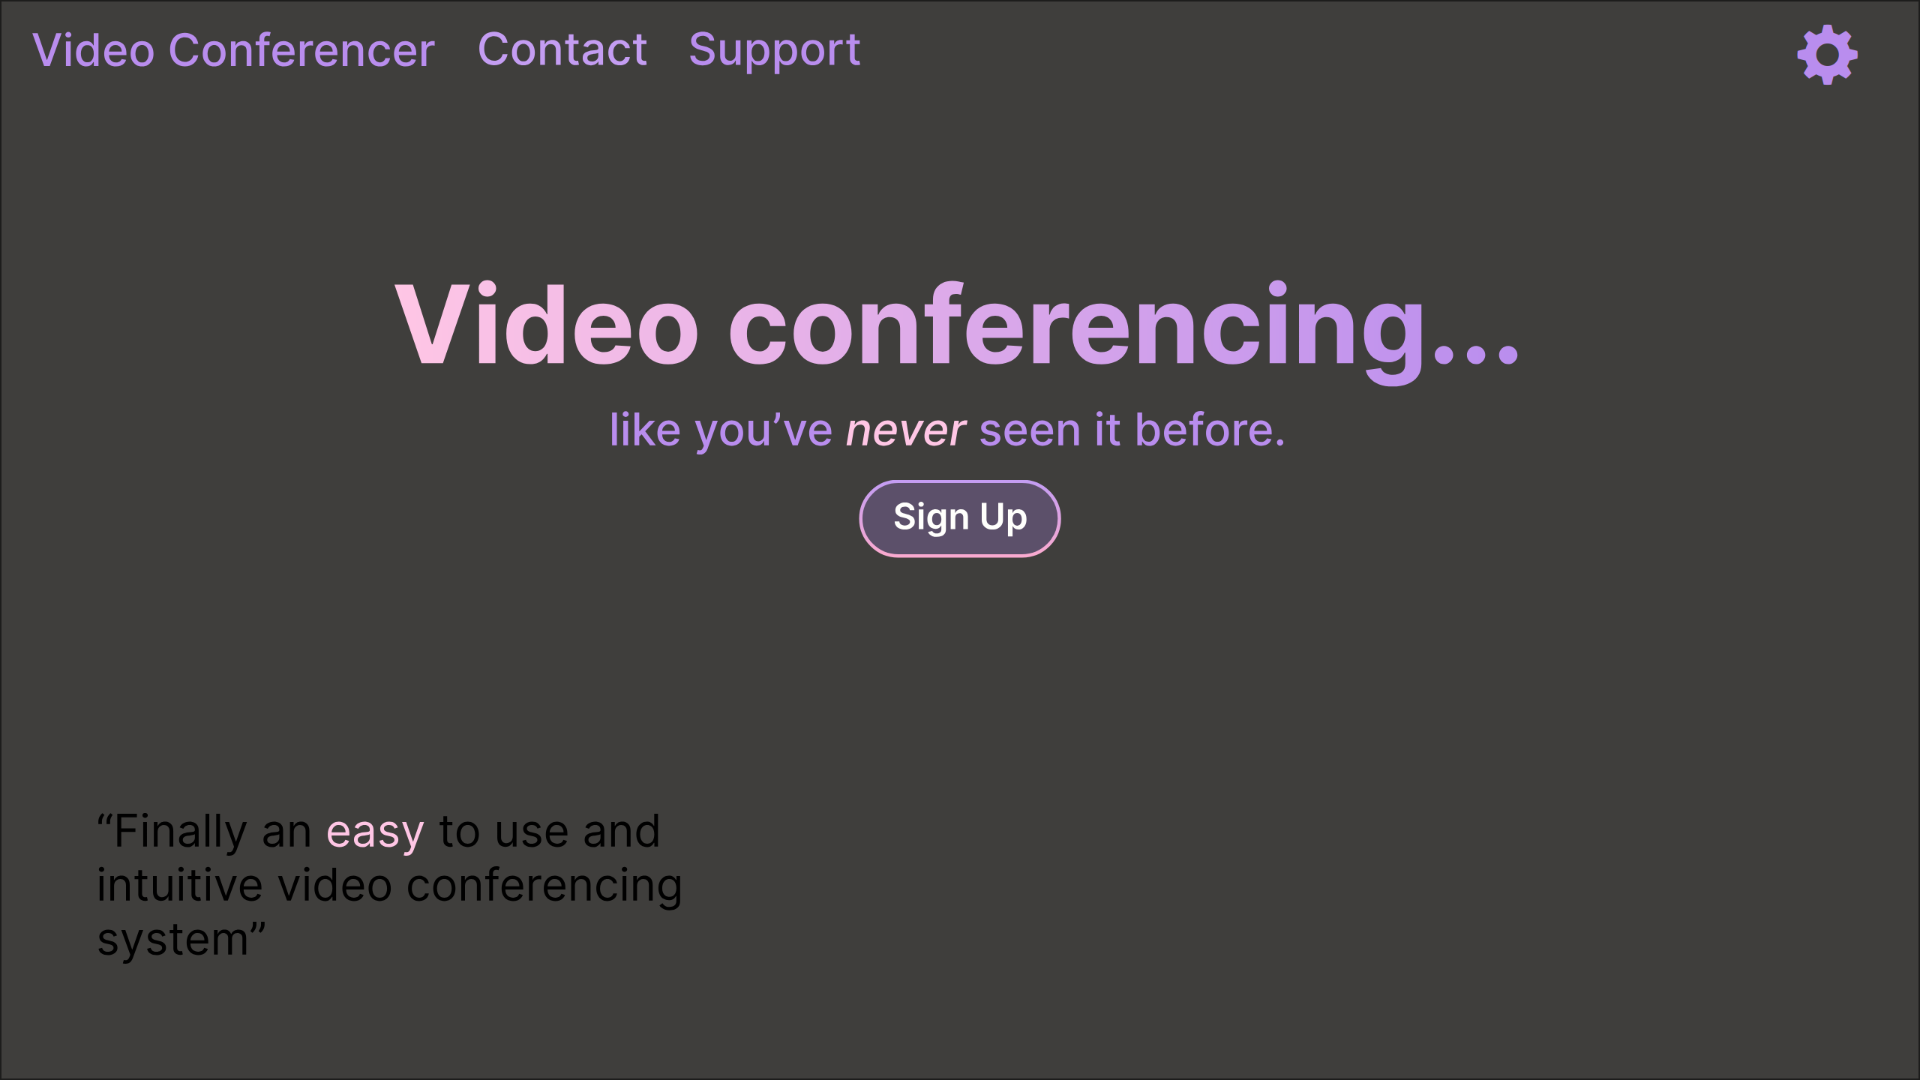
\includegraphics[scale=0.2]{Images/Proto_home3.png}

\caption{Home page prototype 3}
\end{figure}

{\color{gray} \hrulefill} \vspace{0.2cm}

{\sffamily Client feedback:}

\begin{itemize}
  \item Everything looks great!
\end{itemize}

{\color{gray} \hrulefill}

\subsubsection{Refinements}

\textit{Description:}
I reduce the usage of vector graphics in our design,
add a gradient to the background, add a new navigation
tab and more. I conclude by cleaning up some of our CSS
code. \\ \vspace{0.2cm}

\textit{Explanation and justification:}
Not much has changed in terms of the UI of our home
page. I added a soft gradient to out previously plain
gray background as well as a new navigation tab "Docs".
This is where users will click in order to read the
documentation for our back end. I added in 2
more quotes to the bottom of the page, in a card
format using a \texttt{.svg} graphic. I also changed
the navbar to make use of text instead of
\texttt{.svg} images because they are easier to align
and will help the page load faster aswell. Then as a nice
touch I added a simple hover transformation to the sign up
button that makes the whole button a gradient. Finally I
cleaned up the code and made more use of CSS's
viewport and \texttt{margin: auto} properties, since
this would ensure that our users would have the same
UI experience no matter the size of their device. Here
is what the refined code looks like: \\ \vspace{0.2cm}

\underline{main.html}

\begin{minted}[linenos, bgcolor=lightestgray, breaklines, breakanywhere]{html}
...
<body>

  <ul id="Navbar">

    <li class="Navbar_item">
      Video-Conferencer
    </li>

    ...

    <li class="Navbar_item">
      Docs
    </li>

    <li class="Last_Navbar_item">
      <i class="glyphicon glyphicon-cog"></i>
    </li>
  </ul>

  <div id="Main">

    <object id="Headline" data="Images/Headline.svg" type="image/svg+xml">
      <img src="Images/Headline.png">
    </object>

    <button class="Sign_up"> <b> Sign up </b> </button>

  </div>

  <object id="Quote" data="Images/Quote_cards.svg" type="image/svg+xml">
    <img src="Images/Quote_cards.png">
  </object>

</body>

</html>
\end{minted}

\underline{style\_main.sass}

\begin{minted}[linenos, bgcolor=lightestgray, breaklines, breakanywhere]{sass}
@import url('https://fonts.googleapis.com/css?family=Inter')
@import url('https://maxcdn.bootstrapcdn.com/bootstrap/3.3.7/css/bootstrap.min.css')

// Colour definitions
...

// Setting font and background colour
body
  height:           100vh
  margin:           0
  background-image: linear-gradient($Col_Main, $Col_Gradient)
  ...

// Positioning the headline
#Headline
  display:      block
  margin-left:  auto
  margin-right: auto
  ...

// Styling the sign up button
.Sign_up
  border-radius:    700px
  color:            white
  background-color: $Col_Button_BG
  border:           none
  ...

// Creates border and hover effect
.Sign_up::after
  content:          ''
  position:         absolute
  background-image: linear-gradient(to bottom, $Col_Button_Top, $Col_Button_Bot)
  z-index:          -1
  ...

.Sign_up:hover
  z-index: 0

// Styling the navigation bar
#Navbar
  list-style-type: none
  margin:          0
  padding:         0
  ...

.Navbar_item
  color:       $Col_Secondary
  padding:     2vh
  font-size:   2.3vw
  white-space: nowrap

.Last_Navbar_item
  @extend      .Navbar_item
  margin-left: auto

// Positioning the call to action button
#Main
  display:         flex
  align-items:     center
  justify-content: center
  ...

// Positioning the quote
#Quote
  position:    fixed
  bottom:      -27px
  left:        50%
  ...
\end{minted}

This code produced this page:

\begin{figure}[H]
\centering

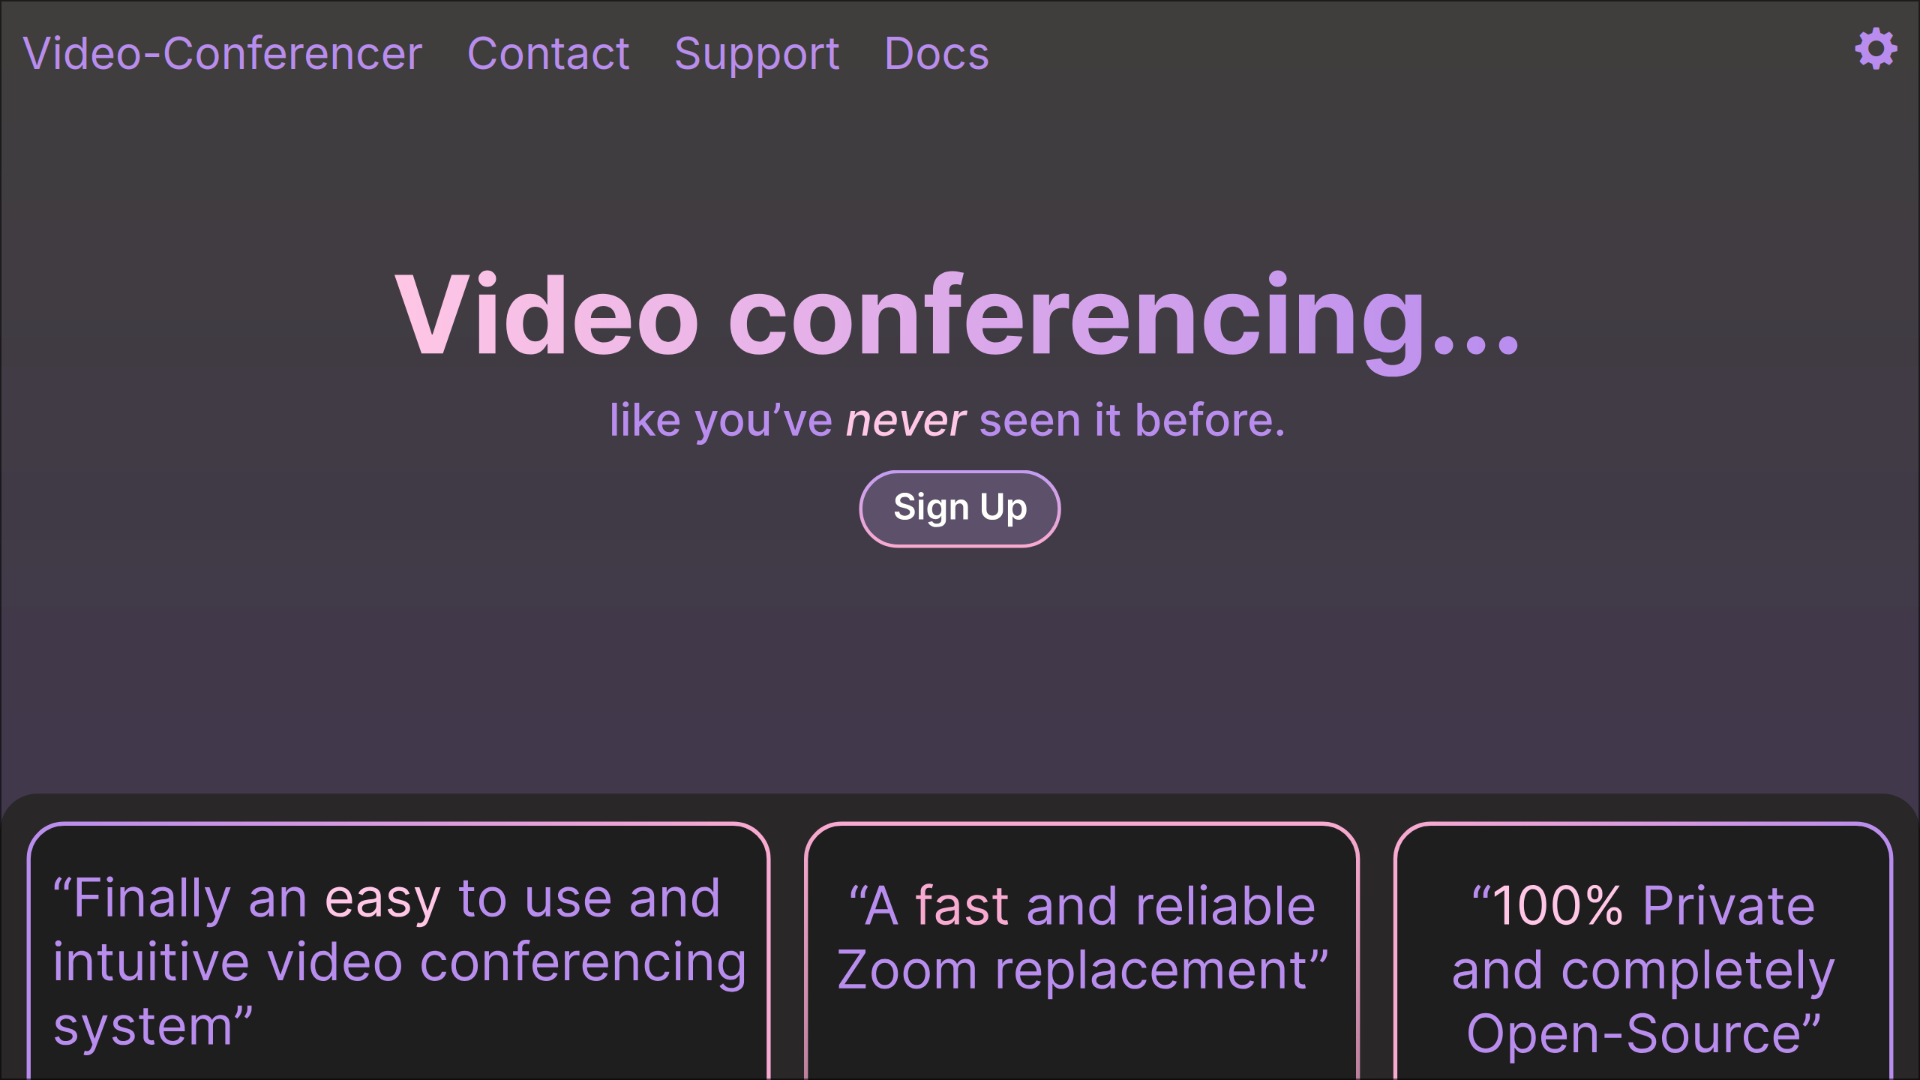
\includegraphics[scale=0.2]{Images/Refined_home.png}

\caption{Refined home page.}
\end{figure}

{\color{gray} \hrulefill} \vspace{0.2cm}

{\sffamily Development sub-task \circled{1} \faCheck}

\subsubsection{Login page}

\textit{Description:} I re-design the login page to fit with the
new theme, and implement my design in HTML and sass.\\ \vspace{0.2cm}

\textit{Explanation and justification:}
Clearly the login page needed to be re-designed also in order
to properly match the theme of the home page. Here is the
revised design for our login page. Inspiration was drawn
from Spline's login UI \url{https://spline.design/}.

\begin{figure}[H]
\centering

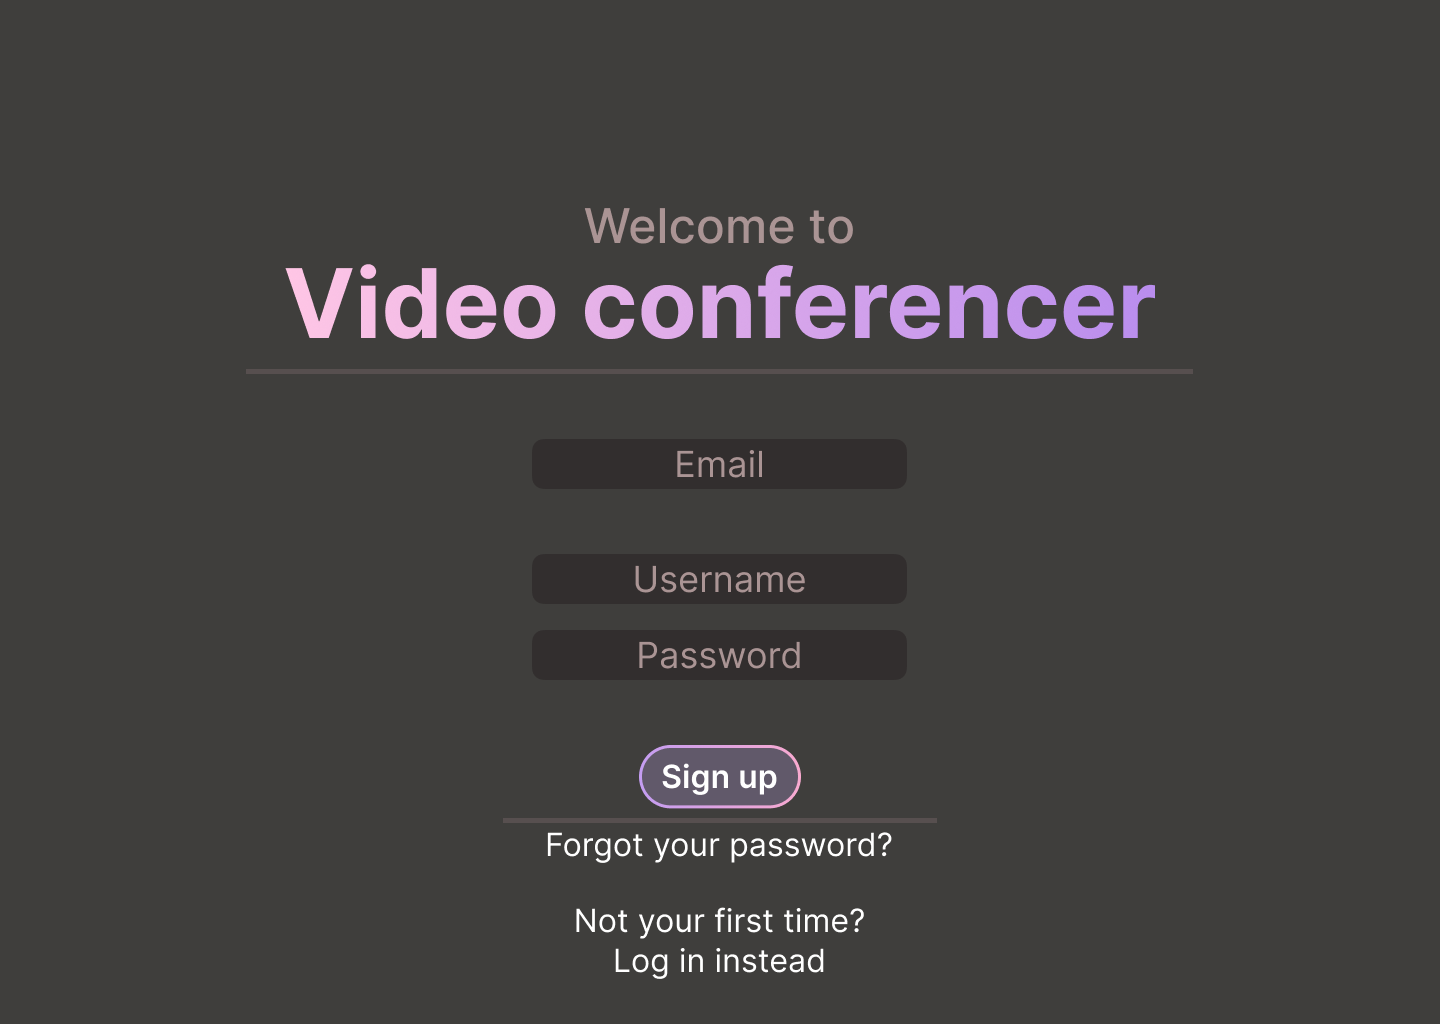
\includegraphics[scale=0.2]{Images/Login_Page_2.png}

\caption{2nd Mock up of the login page.}
\end{figure}

This revised version fits much nicer with the home page.
During the creation of this page however I realised that I
had not yet discussed what we would do if a user had
forgotten their password. In such a case we could employ
the standard technique of sending the user a reset password
link to their email address and I have included this in
our mock up. This idea will have to be added as a development
sub-task and we will tackle it's implementation in a future
iteration. \\ \vspace{0.2cm}

The next step is to transfer the design in code, then link
our home page and login page together. During the programming
of the home page I realised that I would be using the same
sign-up button design as the one designed on the home page.
Recalling that I would apply the DRY
("\textbf{D}on't \textbf{r}epeat \textbf{y}ourself") principle
whilst I wrote my code (see section \ref{sec:computational}),
I decided to put the button code in it's own file
\texttt{button\_styling.sass} and simply have the other \texttt{.sass}
files import from the button styling file whenever needed. Now
that I had gained some experience with translating my designs into
HTML and CSS I was able to make some changes to the design on the
fly to improve upon the figma mock up design. \\ \vspace{0.2cm}

\underline{login.html}

\begin{minted}[linenos, bgcolor=lightestgray, breaklines, breakanywhere]{html}
...
<body>

  <object id="Headline" data="Images/Welcome.svg" type="image/svg+xml">
    <img src="Images/Welcome.png">
  </object>

  <center>
    <b id="Login_Prompt"> Log in instead? Click here </b>
  </center>

  <br><br>

  <center>

    <div id="Login">

      <form>
	<input type="text" placeholder="Email" name="email" required>       <br><br><br>
	<input type="text" placeholder="Username" name="username" required> <br><br>
	<input type="password" placeholder="Password" name="password" required autofocus>
	<br> <br> <br>

	<button class="Button"> <b> Sign up </b> </button> <br><br>

	<div class="Rule"> </div> <br>

	<p style="color:white; font-size: 20px"> Forgot your password? </p>
      </form>
    ...
\end{minted}

\underline{styles\_login.sass}

\begin{minted}[linenos, bgcolor=lightestgray, breaklines, breakanywhere]{sass}
@use './button_styling.sass'
@import url('https://fonts.googleapis.com/css?family=Inter')
@import url('https://maxcdn.bootstrapcdn.com/bootstrap/3.3.7/css/bootstrap.min.css')

// Colour definitions
...

// Setting font and background colour
body
  height:           100vh
  margin:           0
  background-color: $Col_Main
  ...

.Rule
  width: 40%
  border-bottom: 4px solid $Col_Rule

// Positioning the headline
#Headline
  display:      block
  margin-left:  auto
  margin-right: auto
  ...

// Positioning the login box
#Login
  disply:       block
  margin-left:  auto
  margin-right: auto

// Styling the input field
input
  border-radius:    12px
  width:            281px
  height:           37.5px
  ...

#Login_Prompt
  color:     white
  font-size: 20px
\end{minted}

This code produced our first prototype:

\begin{figure}[H]
  \centering
  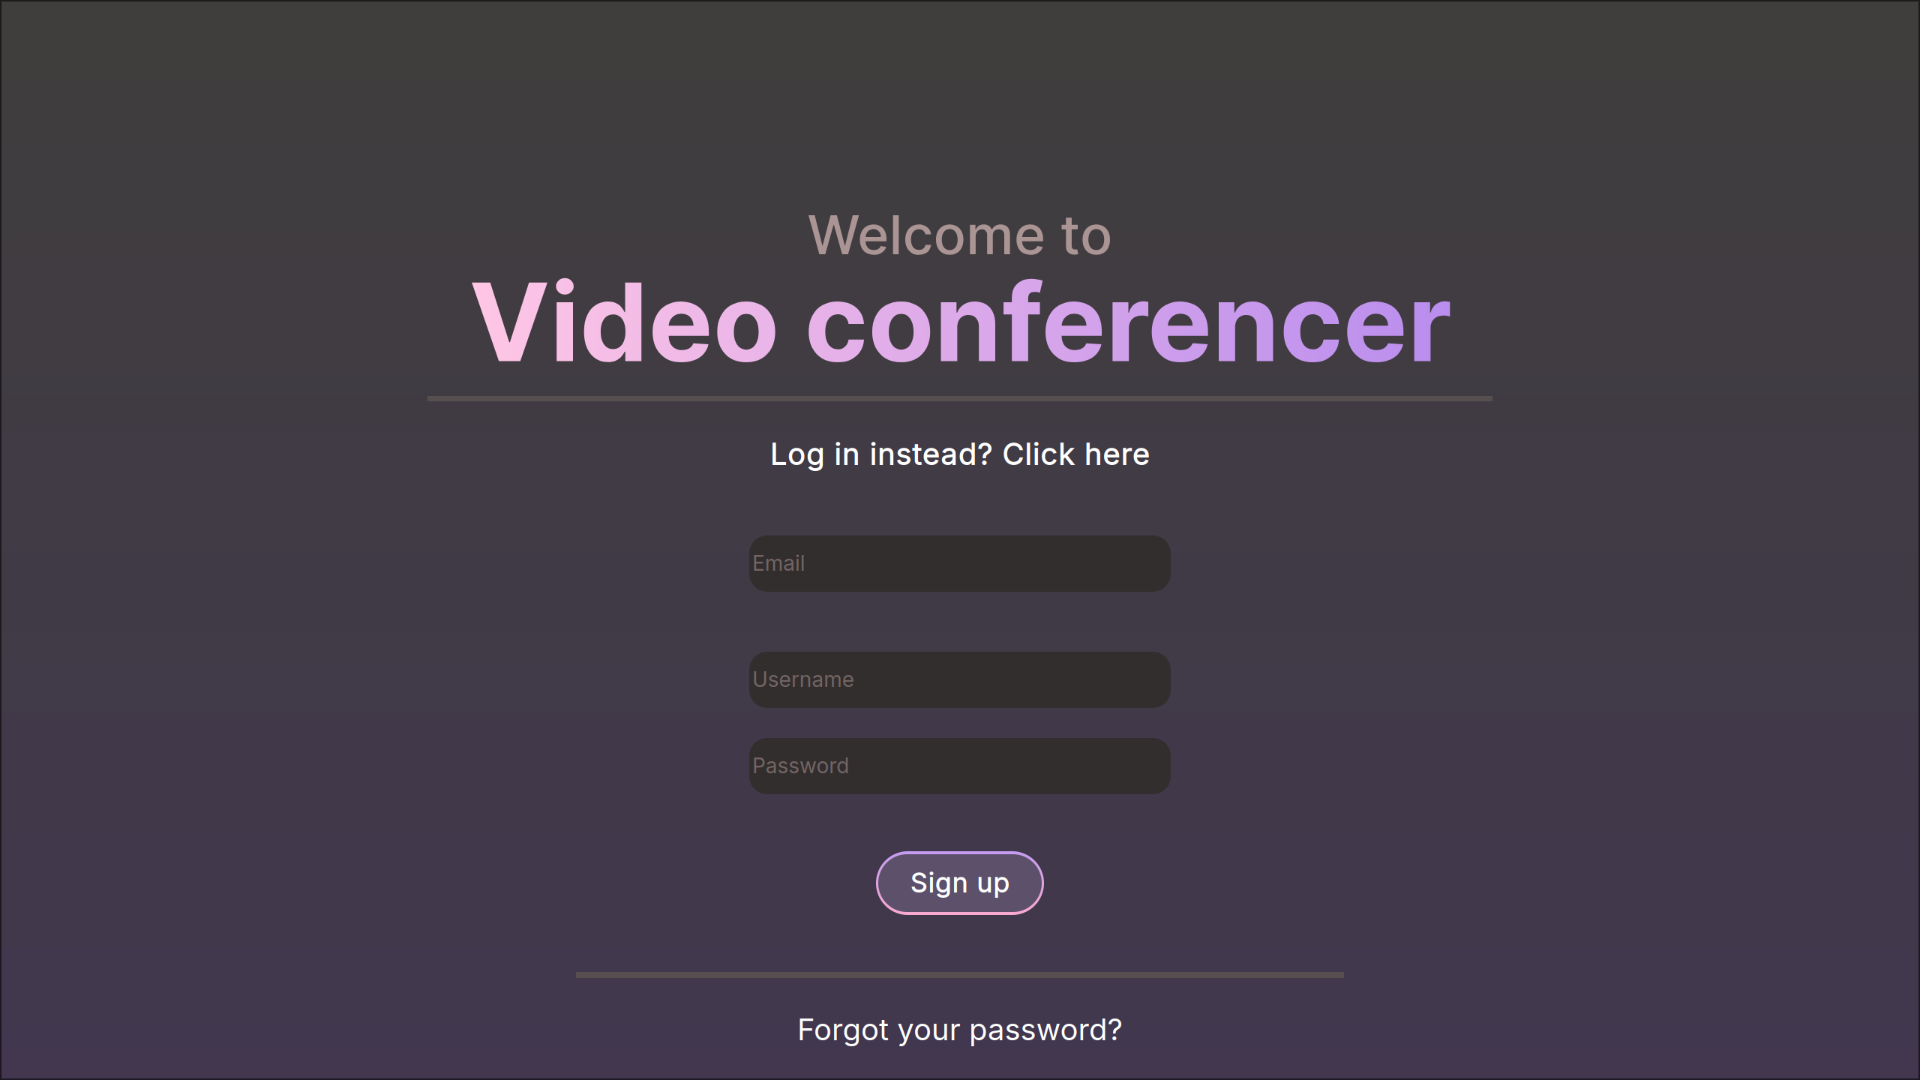
\includegraphics[scale=0.2]{Images/LoginUI.png}
  \caption{Login UI prototype 1}
\end{figure}

{\color{gray} \hrulefill} \\ \vspace{0.2cm}

{\sffamily Client feedback:}

\begin{itemize}
  \item Looks great!
\end{itemize}

{\color{gray} \hrulefill}
\vspace{0.2cm}

{\sffamily Development sub-task \circled{1.2} \faCheck} \\
\vspace{0.2cm}

Look at Github commit
\texttt{54e06ac60f0876086c259f29ce23eae89ff4aad6} to
see the state of the project after our first iteration.\\
\vspace{0.1cm}

Alternatively click the following link to view the state of
the project at this point in development: \\
\href{https://github.com/zzzNathan/Video-Conferencer/tree/54e06ac60f0876086c259f29ce23eae89ff4aad6}{
\texttt{VideoConferencer-Iteration1}}.

\section{Iteration 2}

During this iteration I wanted to design and implement
some of the underlying infastructure behind our application
and complete development subtasks \circled{2} and \circled{A}.\\
\vspace{0.2cm}

\textit{Description:}
After doing some of research into free web deployment
services I settled on using Vercel in order to deploy my website.\\
\vspace{0.2cm}

\textit{Explanation and justification:}
Here are a few of the other options I looked into and why I rejected
them. \\ \vspace{0.2cm}

\begin{tblr}{colspec={XX}, row{1}={lightestgray}}
Service & Explanation \\

Railway.app & You can only use \$5.00 worth of resources on the
free tier, once this is depleted the project won't be up
anymore \\

render.com & Projects on the free tier are deleted automatically after 1 month \\
\end{tblr}

On the other hand Vercel doesn't have any of these drawbacks, so my
site will be able to stay up permanently so long as some resource limits are
not crossed. \\ \vspace{0.2cm}

\textit{Description:} In order to use Vercel to deploy my web
application I had to use a web framework. I chose to use React with
Vite and rewrote my existing codebase to work with this framework. \\
\vspace{0.2cm}

\textit{Explanation and justification:}
Initially I intended to try and stay away from all of these
web-frameworks and just stick to plain old HTML and CSS (or
sass in our case), however an issue arose when I wanted to
redirect users to our registration page once they clicked
the sign up button on our home page. For whatever reason
the redirection would work when I hosted the application on
my own machine, however when I would deploy to vercel the
redirection would either, simply not change page or display
a 404 code not found error.

\begin{figure}[h]
\centering

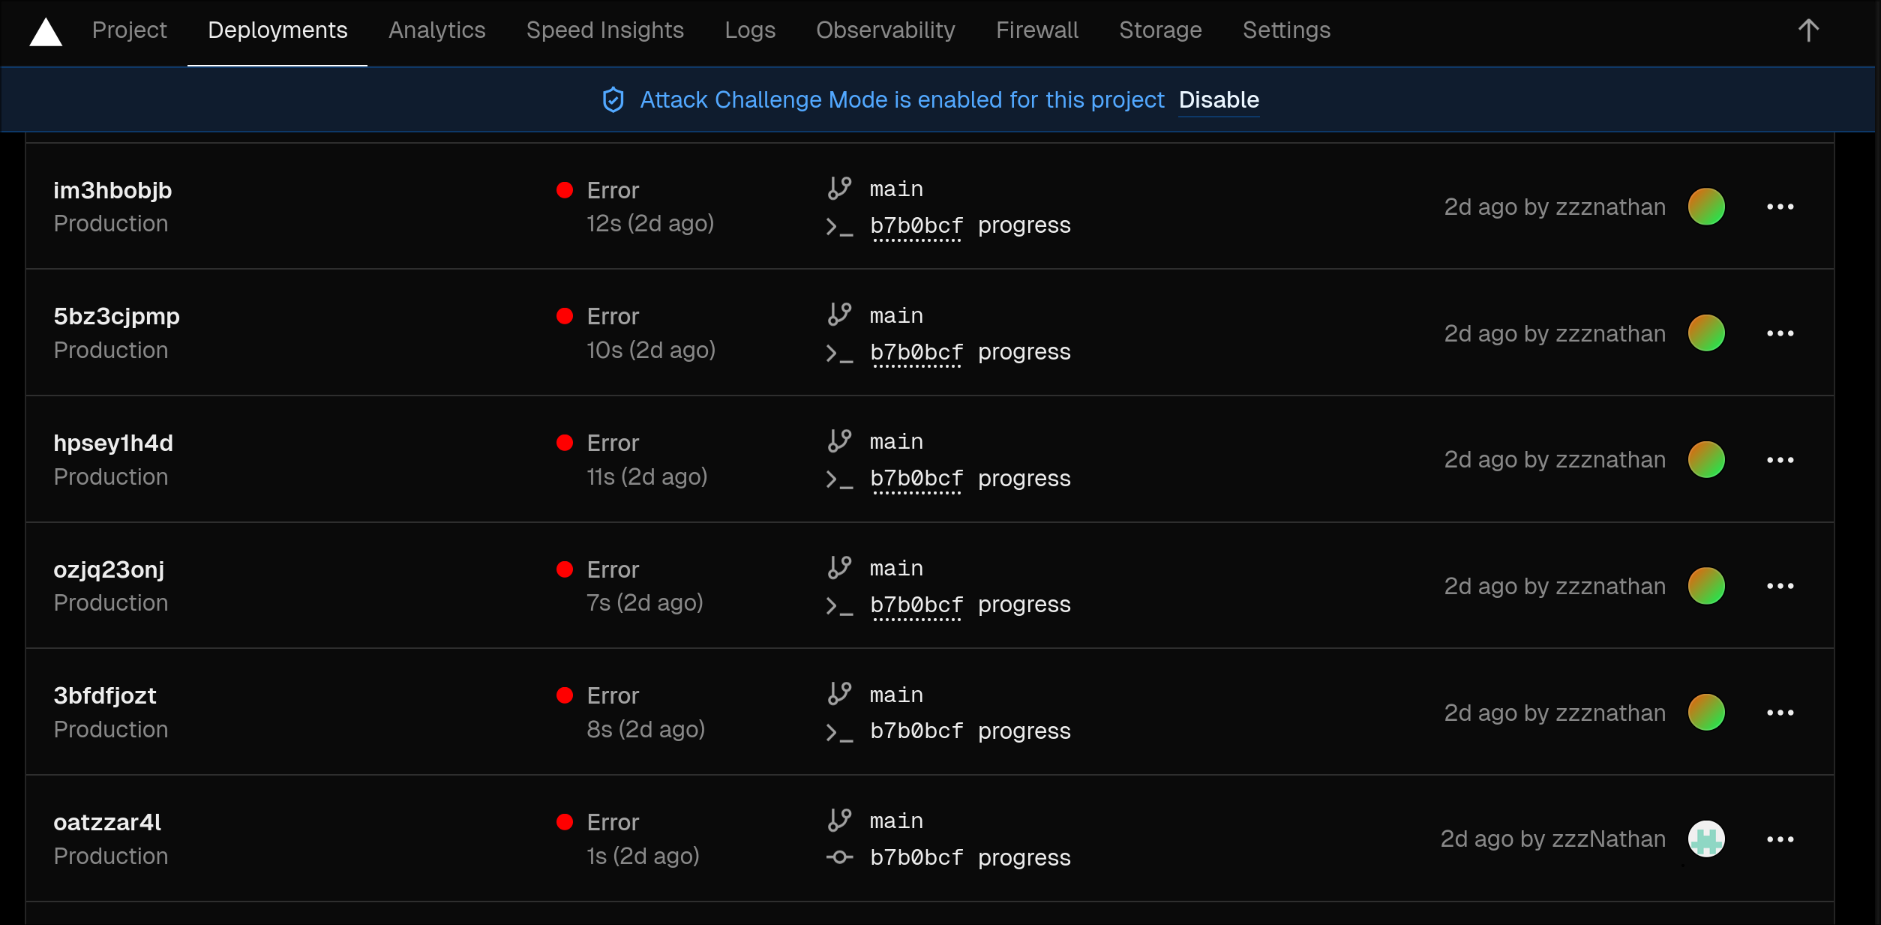
\includegraphics[scale=0.2]{Images/Vercel_Errors.png}

\caption{Errors when deploying to Vercel.}

\end{figure}

Eventually after a lot of trial and error and some research,
I found out that using a router with react would allow us to
redirect the user to different pages once deployed. I then
took some time to migrate our codebase to JSX to work with the
react framework. We will omit the code for the re-written
webpages since it is pretty similar to the snippets shown in
Iteration 1. Here is what the routing logic looks like. \\
\vspace{0.2cm}

\underline{main.jsx} \\ \vspace{0.2cm}

\begin{minted}[linenos, bgcolor=lightestgray, breaklines, breakanywhere]{jsx}
import { createRoot } from "react-dom/client"
import { createBrowserRouter, RouterProvider } from "react-router-dom"
import Home from "./components/Home.jsx"
import Registration from "./components/Registration.jsx"

// Path is an extension that goes after our URL,
// once this extension is written the corresponding
// React element will be loaded and rendered.
const router = createBrowserRouter([
  {
    path: "/",
    element: <Home />
  },
  {
    path: "/registration",
    element: <Registration />
  }
])

createRoot(document.getElementById('root')).render(
  <RouterProvider router={router} />
)
\end{minted}

\textit{Description:} I used the Clerk user management
platform to create a user account registration form.\\
\vspace{0.2cm}

\textit{Explanation and justification:} I originally wanted to
do this task manually, creating my own table and then querying
this table in order to add new users and log users in. However
after doing some reading and looking over Stack Overflow posts
like this one \url{https://stackoverflow.com/questions/46819734/how-to-check-username-and-password-matches-the-database-values}
I realised that many issues can arise when developers try to
implement these systems themselves. In order to avoid this
plethora of issues I instead chose to use the Clerk.com API
\footnote{I originally came across this API watching Theo T3.gg's
React tutorial.}
for user authentication. Not only was it much easier to implement
but the usage of this API also ensures that I wont have to worry
about any security issues, since the API has been thoroughly
tested. Here's the implementation. \\ \vspace{0.2cm}

\underline{Registration.jsx}
\begin{minted}[linenos, bgcolor=lightestgray, breaklines, breakanywhere]{jsx}
import { ReactTyped } from "react-typed"
import { ClerkProvider, SignedOut, SignUp } from "@clerk/clerk-react"
import { dark } from "@clerk/themes"
import Navbar from "./Navbar"
import "../styles/Registration.sass"

const PUBLISHABLE_KEY = import.meta.env.VITE_CLERK_PUBLISHABLE_KEY
...

function Registration () {
  return (
  <> <Navbar />
    <Headline />

    <ClerkProvider publishableKey={PUBLISHABLE_KEY}>
      <SignedOut>
        <center> <SignUp appearance={dark}/> </center>
      </SignedOut>
    </ClerkProvider>
  </>
  )
}

export default Registration
\end{minted}

Here is what the code renders to:

\begin{figure}[H]
\centering

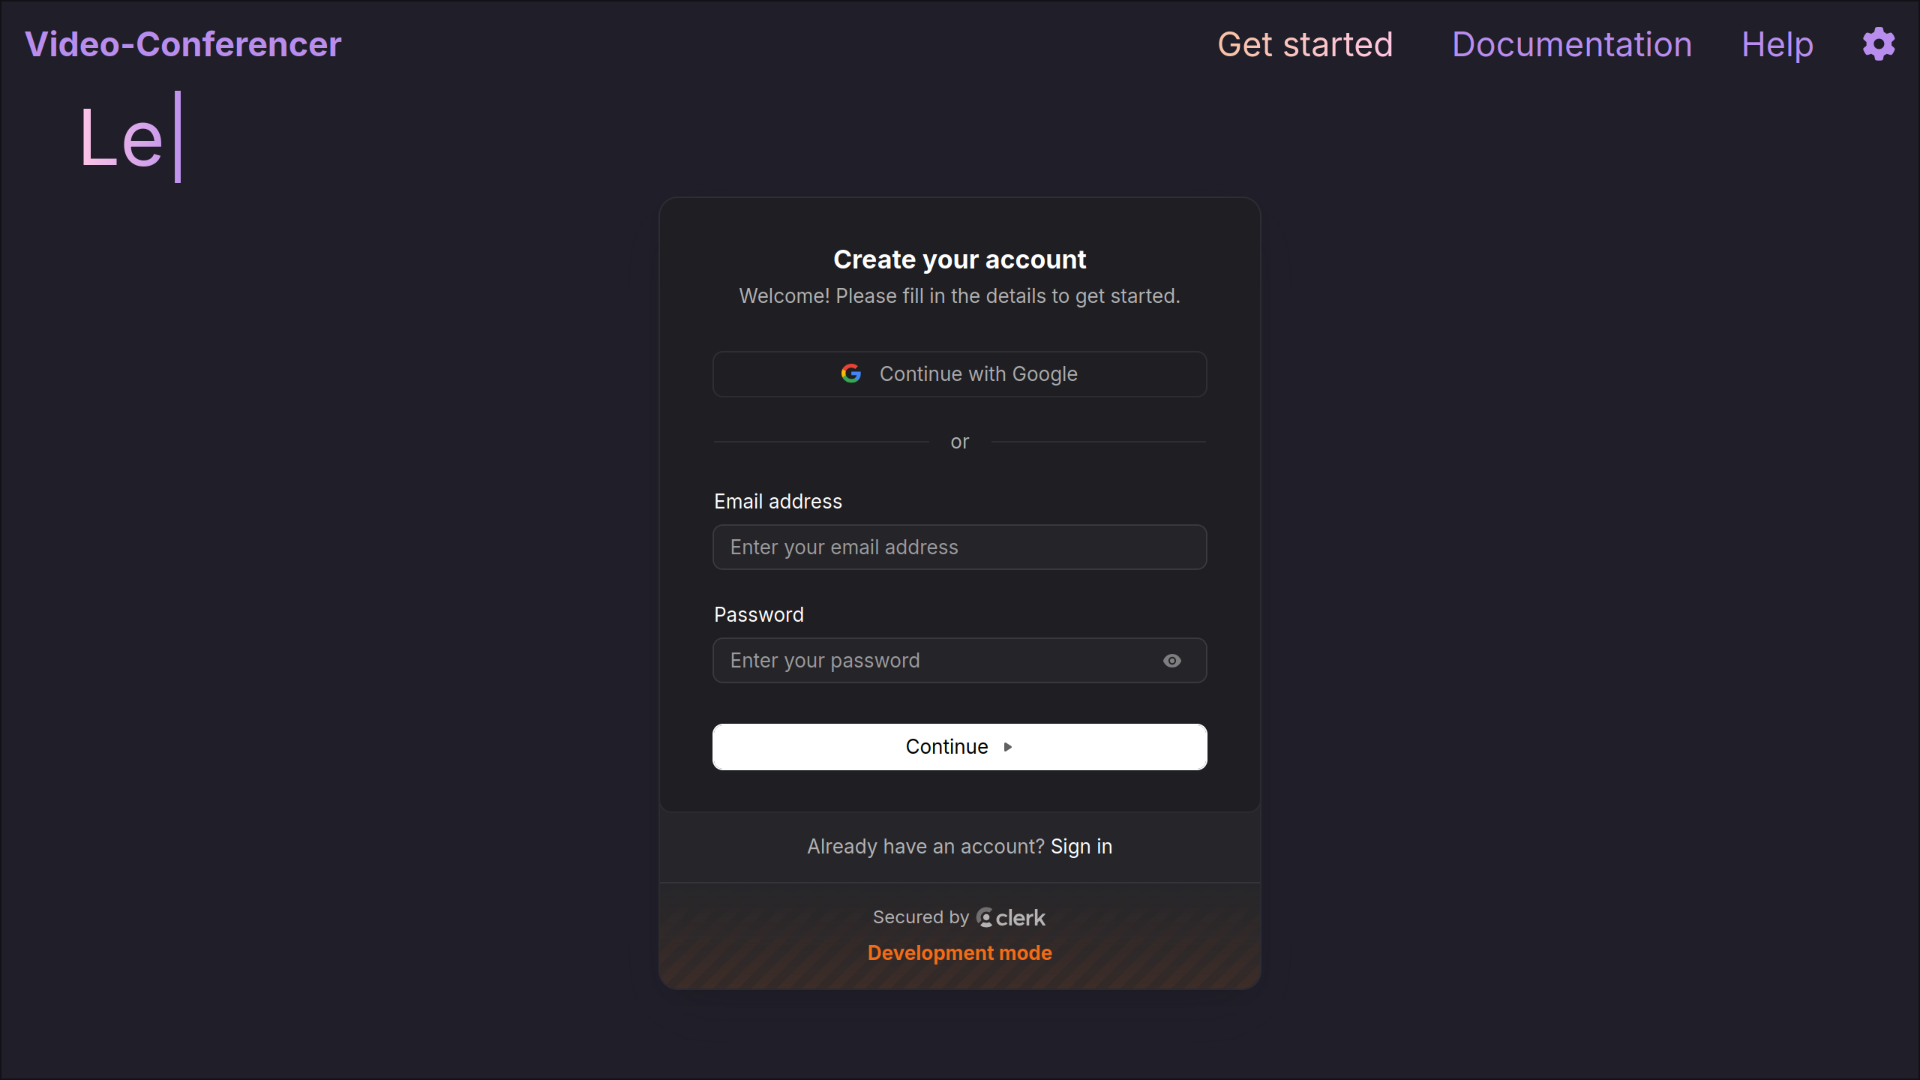
\includegraphics[scale=0.2]{Images/Registration.png}

\caption{Rendering the registration page.}
\end{figure}

{\color{gray} \hrulefill}
\vspace{0.2cm}

{\sffamily Tests: (1)}
\begin{itemize}
  \item Site home page loads correctly \faCheck \\
  \item Correctly redirected to registration page \faCheck \\
  \item Users can create a new account \faClose \\
\end{itemize}

{\sffamily Evidence: \url{https://youtu.be/tHUQeArAv-g}}

{\color{gray} \hrulefill}
\vspace{0.2cm}

The reason why the registration page wasn't rendering was because
I made use of Clerk's \code{useUser()} function in my
\code{<Navbar />} component outside of a ClerkProvider component.
As per the documentation \textit{"The}
\code{<ClerkProvider>} \textit{component is required to integrate
Clerk into your React application, providing session and user
context to Clerk's hooks and components."}
\footnote{Source: https://clerk.com/docs/components/clerk-provider}
This makes sense since
the Clerk SDK would need to have context about the current user
logged in order to get the information returned in the
\code{useUser()} hook, like the \code{user.id} and the
\code{user.username}. \\ \vspace{0.2cm}

This issue was fixed by simply wrapping my HTML code in the
\code{<ClerkProvider>} component whenever a page made usage of the
\code{<Navbar />}. All the tests now successfully pass. \\ \vspace{0.2cm}

Note that with this we have achieved success criteria 5 and 6. \\ \vspace{0.2cm}

{\color{gray} \hrulefill}
\vspace{0.2cm}

{\sffamily Tests: (2)}
\begin{itemize}
  \item Site home page loads correctly \faCheck \\
  \item Correctly redirected to registration page \faCheck \\
  \item Users can create a new account \faCheck \\
\end{itemize}

{\sffamily Evidence: \url{https://youtu.be/IjwQH1Z8aPw}} \\ \vspace{0.2cm}

{\sffamily Input Validation:}
\begin{itemize}
  \item Site doesn't allow users to input weak passwords \faCheck \\
  \item Site doesn't allow users to input email addresses that aren't of the correct format \faCheck \\
\end{itemize}

{\sffamily Evidence: } \url{https://youtu.be/p-rWgn692KU}

{\color{gray} \hrulefill}
\vspace{0.2cm}

You can try these features out yourself at \url{https://video-conferencer.vercel.app/registration}.
(May not work if development is ongoing).\\ \vspace{0.2cm}

{\sffamily Development sub-task \circled{2} \faCheck \\ \vspace{0.2cm}
Development sub-task \circled{A} \faCheck } \\ \vspace{0.2cm}

Look at Github commit \texttt{243560c390c019ab39903850ef3dba99ed98df18} to see the state of the project after our first
iteration. \\ \vspace{0.2cm}

Alternatively click the following link to view the state of
the project at this point in development: \\
\href{https://github.com/zzzNathan/Video-Conferencer/tree/243560c390c019ab39903850ef3dba99ed98df18}{
\texttt{VideoConferencer-Iteration2}}.

\newpage

\section{Iteration 3}

During this iteration I wanted to further develop the backend
infastructure of our application, and start to sketch out the
actual implementation for including video conferencing in our
application. I also improve the code and touch up some of the
designs, and use Clerk to rewrite the login page. With that
we implement tasks \circled{8} and \circled{B} \\ \vspace{0.2cm}

\textit{Description:} I rewrite the login page using clerk,
and make minor improvements to our landing page. \\
\vspace{0.2cm}

\textit{Explanation and justification:} Our users can now
register an account with Clerk, so they will also have to
login using the Clerk SDK aswell. During this time I also
improved the landing page design. These improvements
contribute to the professional look and feel of our website
and enhance the user experience. \\ \vspace{0.2cm}

\underline{Login.jsx}

\begin{minted}[linenos, bgcolor=lightestgray, breaklines, breakanywhere]{jsx}
...
// Makes the typing headline animation
function Headline ()
{
  return (
    <ReactTyped
      className={"Headline"}
      strings={[
        "Welcome back :)",
	"    Log back in here,",
      ]}
      typeSpeed={120}
      startDelay={30}
      loop
    >
    </ReactTyped>
  )
}

// Renders the login page
function Login () {
  return (
  <>
    <ClerkProvider publishableKey={PUBLISHABLE_KEY}>
      <Navbar />
      <Headline /> <br/>
      <SignedOut> <center>

        <SignIn
          signUpUrl="/registration"
          forceRedirectUrl="/home"
          appearance={{
            baseTheme: dark,
            variables: {spacingUnit: "2vh"}
	  }}
	/>

      </center> </SignedOut>
    </ClerkProvider>
  </>
  )
}

export default Login
\end{minted}

Here's what the code renders to: \\

\begin{figure}[H]

\centering
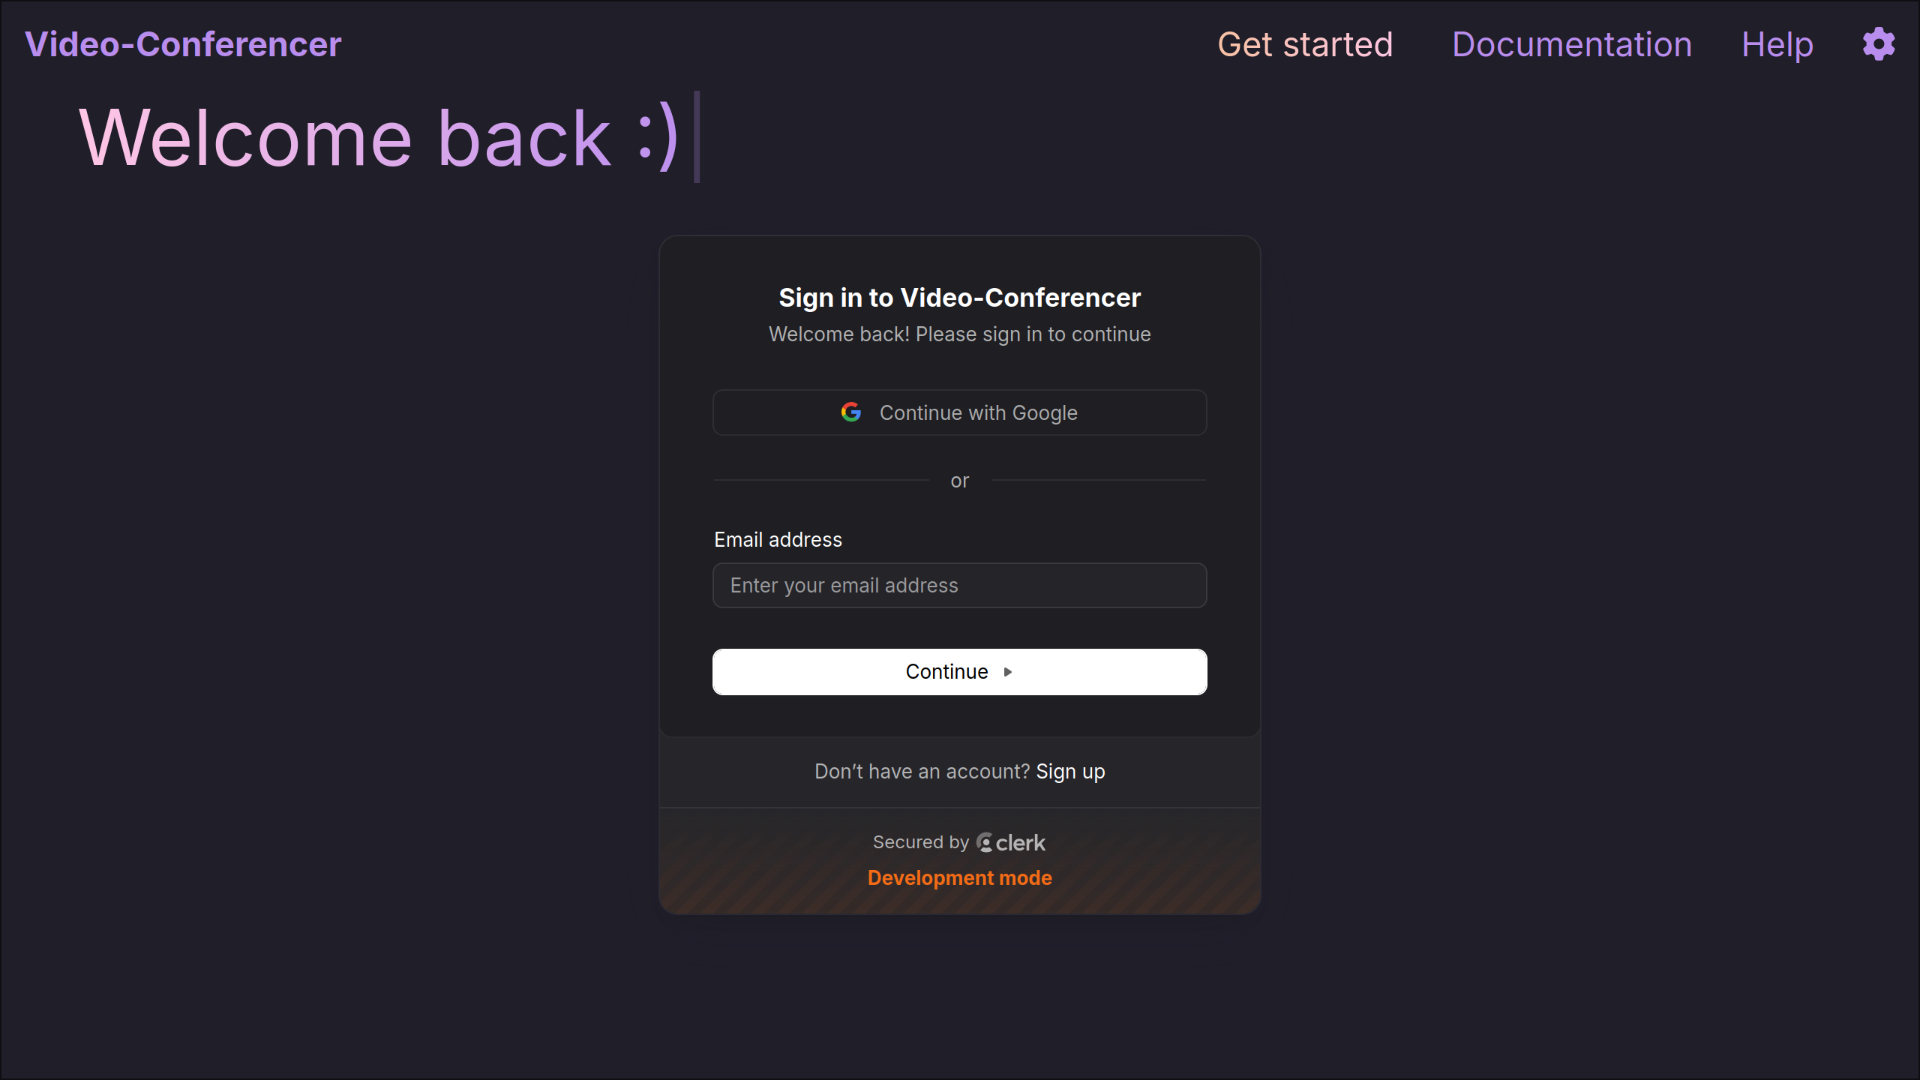
\includegraphics[scale=0.2]{Images/Login.png}

\caption{Rendering the login page.}

\end{figure}

\textit{Description:} I design and implement the page that
users will see after logging in to their account. \\
\vspace{0.2cm}

\textit{Explanation and justification:} In order to start,
join video conferences and change video configuration
settings, the user must have some way to be able to access
these features. The UI should allow our users to easily
navigate the site, providing a good user experience whilst
still looking professional. I began by making a quick sketch
of the design I had in mind. \\

\begin{figure}[h]
\centering

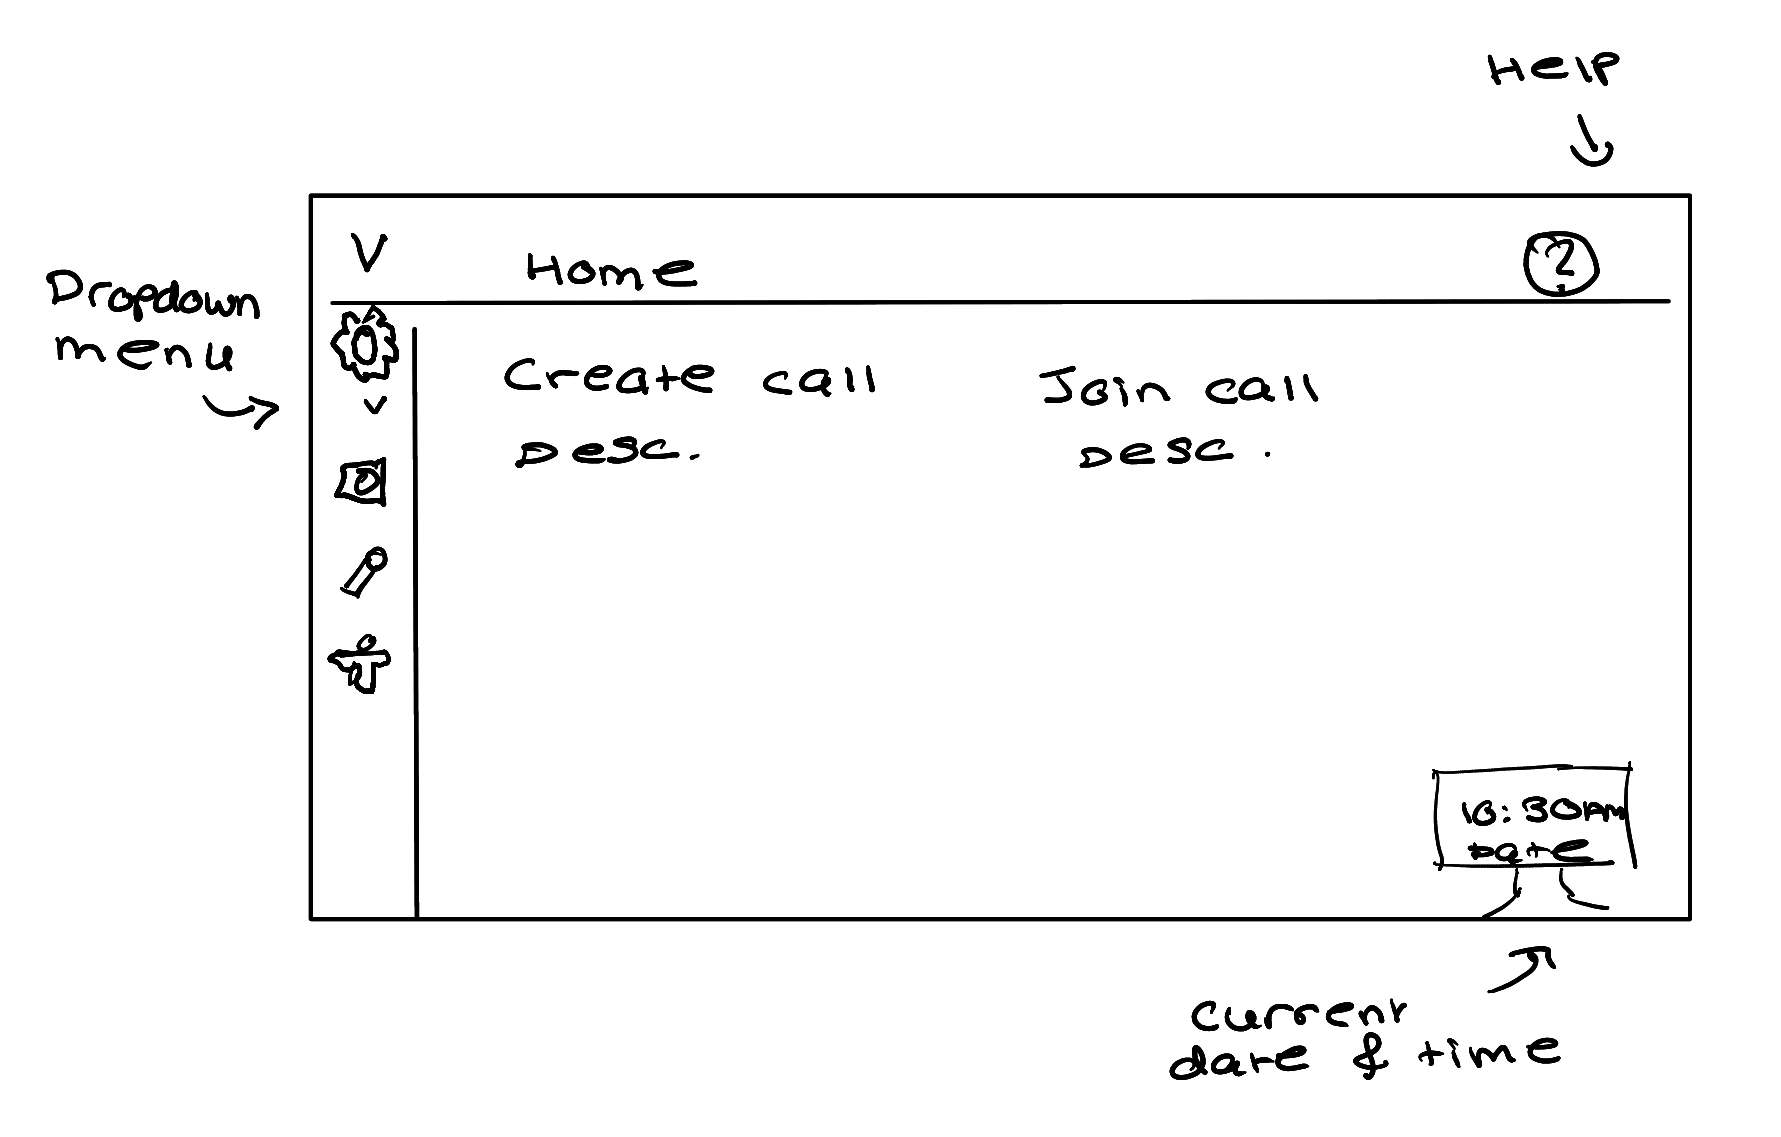
\includegraphics[scale=0.2]{Images/Home_sketch.png}

\caption{Sketching out the design.}
\end{figure}

From here it was pretty simple to write out the code to make
this UI. \\ \vspace{0.1cm}

\textit{Confusingly from here on we call this page
our home page and the page previous home page our landing
page in our code base. In this document we will use the
following names. We will call the page that the user first
sees our 'home' page, we will call the page that the user
first sees after logging in our 'main' page.} \\
\vspace{0.2cm}

\underline{Home.jsx}

\begin{minted}[linenos, bgcolor=lightestgray, breaklines, breakanywhere]{jsx}
import "../styles/Home.sass"
import Clock from "./Clock.jsx"
...

function Options () {
  const Create_Desc = <div className="Desc">
    Create a new video call, then invite others
    to join by giving them the call code given
    to you once you start the call.
  </div>

  const Join_Desc = <div className="Desc">
    Enter the code given to you to join the
    video call.
  </div>

  return (
    <ul className="Options">
      <li> Create call <br/> {Create_Desc} </li>
      <li> Join call   <br/> {Join_Desc}   </li>
    </ul>
  )
}

function Home () {
  return (
    <> <Top_Bar />
    <Side_Bar />
    <Options />

    <Clock />
    </>
  )
}

export default Home
\end{minted}

\begin{figure}[H]
\centering

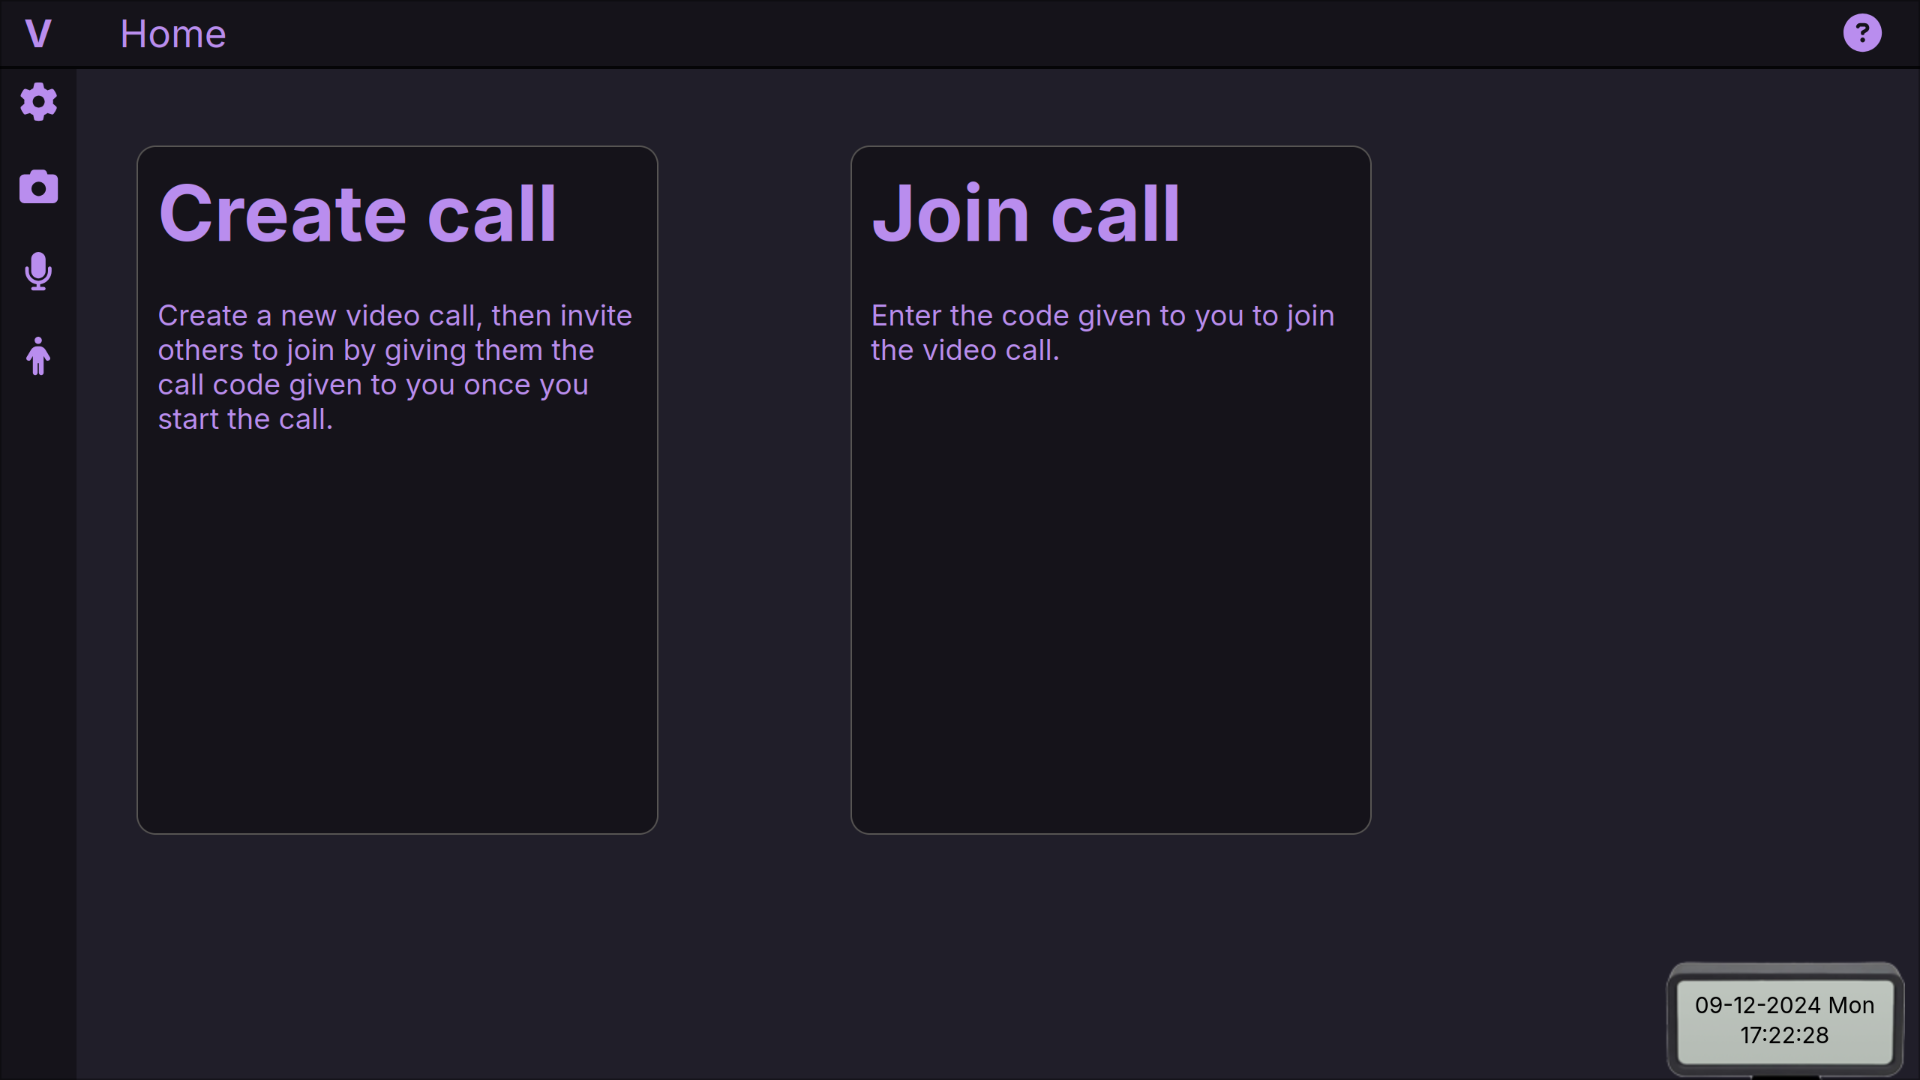
\includegraphics[scale=0.2]{Images/Sketch_final.png}

\caption{Implementing the code for the sketch.}
\end{figure}

\textit{Description:} I chose to use the GetStream React
library to implement video conferencing in my application. \\
\vspace{0.2cm}

\textit{Explanation and justification:} As detailed in my research, I first
intended to use the WebRTC framework provided by Google to
write the video conferencing logic. However after some research
into what it would take for me to implement such a system I
realised that actually implementing the logic would take me
an unreasonable amount of time. Taking into consideration the
fact that I would have to understand and correctly implement
the sending of SDP protocol offers, connecting each user to a
STUN server, whilst ensuring that each user has access to
the other user's ICE candidates, the task felt as though it
would take me a number of weeks to implement such a system
to allow 2 users to video conference properly, let alone have
$n$ users video conference simaltaenously. So instead I chose
to use a popular industry standard video conferncing library
called GetStream. \\ \vspace{0.2cm}

The first step to have users be able to
video conference was to have our users be authenticated as
users on the GetStream API. According to the documentation
in order to do this each user must be given a unique JWT
(JSON web token) token via GetStream's
\code{client.generateUserToken()} function. In the documentation
it explicitly says \textit{"Tokens need to be generated server-side,
... You need to implement the token provider in your own application,
this is usually an HTTP endpoint."} \footnote{Source:
\url{https://getstream.io/video/docs/api/authentication/}}
In order to run the backend code I would need a server or some
other place to be able to host my code. After reading through
some forums online I came across Cloudflare's Worker service.
This service allows users to be able to run server side code
remotely through one of Cloudflare's many servers across the globe,
with pretty generous free tier limits. I quickly set up an account
with Cloudflare and began to implement my HTTP API. \\ \vspace{0.2cm}

\underline{/backend/stream-token-provider/src/index.js} \\

\begin{minted}[linenos, bgcolor=lightestgray, breaklines, breakanywhere]{js}
...

// An HTTP endpoint that allows POST requests
// with a user id given in the request. Will return
// a unique user token that can be used to begin
// video conferencing
async function Provide_Token(request, env)
{
  const { method } = request;

  // Ensure that the request is a POST
  if (method !== 'POST')
    return new Response('Method not allowed', { status: 405 });

  try {
    const { User_Id } = await request.json();

    // Ensure that a valid user id is actually provided
    if (!User_Id || User_Id.length != USER_ID_LENGTH)
      return new Response('Bad Request: Proper userId is required', { status: 400 });

    const apiKey = env.STREAM_API_KEY;
    const secret = env.STREAM_API_SECRET;

    const token = await Generate_Token(User_Id, apiKey, secret);

    return new Response(JSON.stringify({ token }), {
      headers: { "Content-Type": "application/json" },
    });

  } catch (error) {
      return new Response(`Error: ${error.message}`, { status: 500 });
  }
}
...
\end{minted}

{\color{gray} \hrulefill} \\ \vspace{0.2cm}
{\sffamily Tests: (3)}

\begin{itemize}
  \item HTML endpoint is accessible \faCheck \\
  \item Only POST requests are allowed \faCheck \\
  \item A GetStream token is actually provided in the output \faCheck
\end{itemize}

{\sffamily Evidence: \url{https://youtu.be/Ia1knGrbcaE}}

{\color{gray} \hrulefill}
\\ \vspace{0.2cm}

\textit{Description:} I add user id validation to our backend.
\\ \vspace{0.2cm}

\textit{Explanation and justification:} There was no information
to be found on the way that Clerk formats it's user id's, so the
user id validation we can do is quite limited. We simply check
whether or not the string length $s$ satisfies $0 < s \leq 512$.
\\ \vspace{0.2cm}

\begin{minted}[linenos, bgcolor=lightestgray, breaklines, breakanywhere]{js}
...
const MAX_USER_ID_LENGTH = 512
...
// Validate the user id given is correct
function Validate_User_Id(User_Id)
{
  if (User_Id.length > MAX_USER_ID_LENGTH ||
      User_Id.length == 0)
    return false

  return true
}
...
\end{minted}

\textit{Description:} I fix a bug with button misalignment on
mobile. \\ \vspace{0.2cm}

\textit{Explanation:} Whilst testing out how my website works
on different devices, I found that although the page looks
fine on desktop, on mobile the buttons on the home page seem
to be misaligned. \\

\begin{figure}[h]
\centering

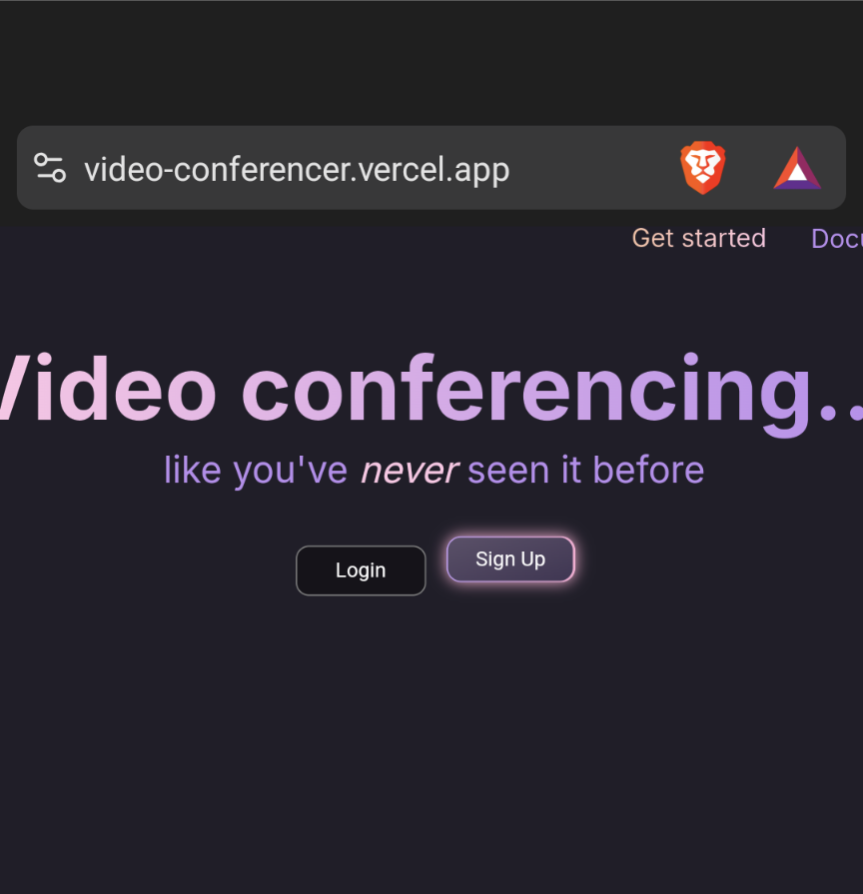
\includegraphics[scale=0.2]{Images/Button_misalignment.png}

\caption{Buttons being misaligned on mobile}
\end{figure}

In order to fix this I simply changed the sass of the login
button to use a pseudo element for it's border, so that it is
created in the same way the sign up button is created. By
doing it this way we can be 100\% sure that both buttons will
now be the same exact size, and that hence we will have no
more alignment issues. \\ \vspace{0.2cm}

\underline{Landing.sass}

\begin{minted}[linenos, bgcolor=lightestgray, breaklines, breakanywhere]{sass}
...
.Login_Button
  border-radius:    0.9vw
  color:            white
  background-color: $Col_Black
  ...

.Login_Button::after
  content:          ''
  position:         absolute
  height:           107%
  ...

.Login_Button:hover
  scale: 104%
...
\end{minted}

These changes fixed our issues with button misalignment.

\begin{figure}[H]
\centering

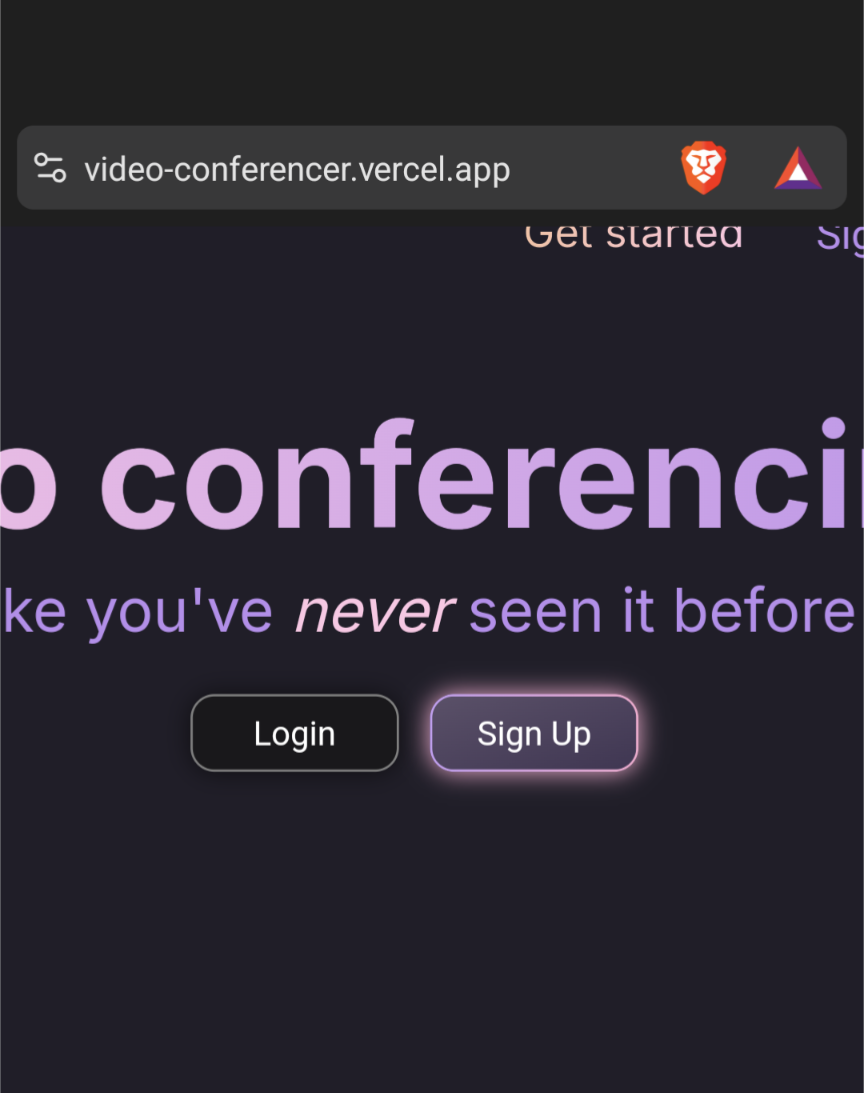
\includegraphics[scale=0.2]{Images/Buttons_aligned.png}

\caption{Buttons being fixed on mobile}
\end{figure}

\textit{Description:} We create another Cloudflare worker to
generate unique call ids. These ids will be used to invite
other users to join one's video conference. \\ \vspace{0.2cm}

\textit{Explanation and justification:} We start by discussing
exactly \textit{how} we are going to generate then distribute
these call ids. As for the format of call ids I decided to
use a 6 digit code \footnote{In reality we exclude the use
of the code \texttt{000000}. This difference is negligable
in our calculations}, providing us with $10^6$ unique call
codes. Note that we can easily increase the number of unique
call codes by allowing ascii characters to used in the call
codes. As users create calls using these ids we would need to
store information in a database to track which call ids are
in use and which call ids are currently available.
\\ \vspace{0.2cm}

An obvious naive algorithm would be to iterate over all call
ids, and individually check whether each one is currently
available. This algorithm would have a worst case time
complexity of $O(n)$ where $n$ is the number of unique call
ids we have, in this case $n = 10^6$. Since each iteration we
are making a call to a database hosted on the cloud, this
could potentially become a pretty time consuming.
\\ \vspace{0.2cm}

One interesting heuristic could be used to optimise the
performance of our current algorithm. Instead of iterating
over we could use a psuedo-random number generator (PRNG) to
\textit{guess} which call ids are currently available. Indeed
as the number of used call ids $k \leq n$ increases the chance
that we successfully randomly generate an available call id
decreases. Let $G$ be the event that we are investigating.
The probability that we successfully guess an available call
id each time is given by,

$$
  Pr(G) = \frac{n-k}{n} = 1 - \frac{k}{n}
$$

Once the database becomes densely populated, this heuristic
becomes more and more unlikely to yield performant results.
\\ \vspace{0.2cm}

Since the heuristic has a higher chance of yielding results
with a sparse database and the naive algorithm runs in
deterministic time, we could combine these 2 algorithms to
extract the best of both worlds. \\ \vspace{0.2cm}

\begin{algorithm}[H]
\caption{Pseudo-code for a call id generation algorithm.}
\sffamily

\begin{algorithmic}[1]
  \Function{Generate\_Call\_Id}{}
    \Let{Taken}{Number of taken call ids}
    \Let{Total}{$10^6$}

    \State{}

    \If {Taken $/$ Total $\leq 0.25$}
      Generate\_PRNG()
    \EndIf

    \State{}

    \State{\textbf{else} Generate\_Linear()}

  \EndFunction
\end{algorithmic}
\end{algorithm}

\mdseries

When getting into the details of implementing this algorithm
in our backend, since we were already using Cloudflare workers
I decided to make use of Cloudflare's D1 database service to
host our database on the cloud. I wrote a function
to make the implementation of our algorithm go smoother. The
utility function I wrote was the \code{Count\_Elements()} function.
It is a function written to count the number of call ids
currently in use and has an optional arguement \texttt{id}, if
an integer \texttt{id} is provided the function will instead
count the number of call ids in our table with a value of
\texttt{id}. For example if I make the call
\code{Count\_Elements(23)} the function returns the number of
records whose \texttt{id} is 23 in our table. The implementation
is as follows,

\begin{minted}[linenos, bgcolor=lightestgray, breaklines, breakanywhere]{js}
...
// Function to count the number call ids in use
// If the id arguement is passed in then function will
// count the number of call ids equal to the arguement
async function Count_Elements(env, id = null)
{
  var query = `SELECT COUNT(id) FROM ${TABLE_NAME}`

  // If id arguement is passed return the number of ids
  if (id !== null) query += ` WHERE id = ${id}`

  const result = await env.DB.prepare(query).run()

  // Get count from JSON format
  const count = result.results[0]["COUNT(id)"]

  return count
}
\end{minted}

{\color{gray} \hrulefill} \\ \vspace{0.2cm}

{\sffamily Tests: (4)}

\begin{itemize}
  \item HTTP endpoint is accessible \faCheck \\
  \item Function successfully returns the number of call ids in use \faCheck \\
  \item Function successfully returns the number of call ids in use where \texttt{id} is a given value \faCheck \\
\end{itemize}

{\sffamily Evidence:} \url{https://www.youtube.com/watch?v=piCR-SANG3o}\\ \vspace{0.2cm}

{\color{gray} \hrulefill} \\ \vspace{0.2cm}

Next I proceeded to write the \code{Generate\_PRNG()}
function. In Javascript there is no built-in function to
generate a random integer in a given interval rather we
are only provided with the \code{Math.random()} function
which generates a floating point number $n \in [0, 1)$.
We now derive a formula for generating a random integer
number using the built-in random function from JS. \\ \vspace{0.2cm}

Let the \code{Math.random()} function be modelled by
the uniformly distributed continous random variable
$X \in [0, 1)$. Indeed by considering the expression
$cX, (c \in \mathbb{N})$ we can see that the
expression will now lie in the interval $[0, c)$. Then by
applying the floor function
$\left \lfloor {cX} \right \rfloor$ we can force
$\left \lfloor {cX} \right \rfloor \in \mathbb{Z}_{\geq 0}$
or more precisely
$\left \lfloor {cX} \right \rfloor \in [0, c-1]$. We have
made some progress however we don't want to have our lower
bound be 0, we want it to be 1 (see the previous footnote).\\
\vspace{0.2cm}

It is often the case in math, that the generalisation of a
problem is easier to solve than the real problem at hand.
George Polya puts it nicely in his book \textit{How to solve
it}. \textit{"The more ambitious plan may have more chances
of success."} \\ \vspace{0.2cm}

Let our desired lower bound be $l \in \mathbb{N}$, and our desired upper
bound be $u \in \mathbb{N}$. Since we have a way to map $[0, 1) \mapsto
[0, t-1], (t \in \mathbb{N})$ why dont we try and \textit{shift}
this interval to become $[l, u]$. If the interval $[0, t-1]$ is the
same size as the interval $[l, u]$ there should exist some $\Delta \in \mathbb{Z}_{\geq 0}$
such that $[0 + \Delta, (t-1) + \Delta] = [l, u]$. As the length of the
interval $[l, u]$ is $u - l + 1$ we should set $t-1 = u - l$
(since the interval $[0, t-1]$ starts from 0). Then we want to find
the $\Delta$ such that $[0 + \Delta, (u - l) + \Delta] = [l, u]$.
We can now see that we need $0 + \Delta = l$ so clearly
$\Delta = l$. \\ \vspace{0.2cm}

Putting all of this together our final expression becomes
$\left \lfloor tX \right \rfloor +l = \left \lfloor (u - l + 1)X \right \rfloor + l$.
This guarentees that we generate random integers
in the interval $[l, u]$. The implementation looks like so,

\begin{minted}[linenos, bgcolor=lightestgray, breaklines, breakanywhere]{js}
...
// Generates a call id using a PRNG
async function Generate_PRNG(env)
{
  var Is_Taken = true

  while (Is_Taken)
  {
    // Since JS returns random numbers in the interval [0, 1)
    var rand = Math.floor(Math.random() * (MAX_ID - MIN_ID + 1)) + MIN_ID

    // If id is unused stop iterating
    if (await Count_Elements(env,rand) == 0) Is_Taken = false
  }

  return rand
}
\end{minted}

{\color{gray} \hrulefill} \\ \vspace{0.2cm}

{\sffamily Tests: (5)}

\begin{itemize}
  \item HTTP endpoint is accessible \faCheck \\
  \item Function successfully returns a random call id \faCheck \\
  \item Function doesn't return an id that is currently in use \faCheck \\
\end{itemize}

{\sffamily Evidence:} \url{https://youtu.be/RgGxgbNYjKQ}\\ \vspace{0.2cm}

{\color{gray} \hrulefill} \\ \vspace{0.2cm}

The next algorithm I wrote was the \code{Generate\_Linear()}
function. This was a rather trivial function to write,

\begin{minted}[linenos, bgcolor=lightestgray, breaklines, breakanywhere]{js}
...
// Generates a call id in linear time
async function Generate_Linear(env)
{
  // If element is not taken then we can return it
  for (let id = 1; id <= MAX_ID; id++)
    if (await Count_Elements(env, id) == 0) return id
}
\end{minted}

{\color{gray} \hrulefill} \\ \vspace{0.2cm}

{\sffamily Tests: (6)}

\begin{itemize}
  \item HTTP endpoint is accessible \faCheck \\
  \item Function successfully returns the next available id \faCheck \\
  \item Function doesn't return an id that is currently in use \faCheck \\
\end{itemize}

{\sffamily Evidence:} \url{https://www.youtube.com/watch?v=7ThFXmu0_98}\\ \vspace{0.2cm}

{\color{gray} \hrulefill} \\ \vspace{0.2cm}

Finally putting all of this together we implement algorithm 7.

\begin{minted}[linenos, bgcolor=lightestgray, breaklines, breakanywhere]{js}
...
// Function to generate a unique call id
async function Generate_Call_Id(env)
{
  var unique_id = 0

  if (await Count_Elements(env) / TOTAL_NUM_IDS <= 0.25)
    unique_id = await Generate_PRNG(env)

  else unique_id = await Generate_Linear(env)

  // Once the unique call id has been generated
  // we must add it to the database to mark that it is in use
  const query  = `INSERT INTO ${TABLE_NAME} VALUES (${unique_id})`
  const result = await env.DB.prepare(query).run()

  return new Response(unique_id, { status: StatusCodes.OK })
}
\end{minted}

{\color{gray} \hrulefill} \\ \vspace{0.2cm}

{\sffamily Tests: (7)}

\begin{itemize}
  \item HTTP endpoint is accessible \faCheck \\
  \item Function successfully returns a call id that isn't in use \faCheck \\
  \item Function then adds that call id to our database \faCheck \\
\end{itemize}

{\sffamily Evidence:} \url{https://youtu.be/5QPmgv1PcuA}\\ \vspace{0.2cm}

{\color{gray} \hrulefill} \\ \vspace{0.2cm}

Once a video call has finished we also need a way to
remove a call id from our database. We use the same
Cloudflare worker to perform this task. Here is the
implementation,

\begin{minted}[linenos, bgcolor=lightestgray, breaklines, breakanywhere]{js}
...
// Function to remove a unique call id from the
// database once a call has finished
async function Remove_Call_Id(request, env)
{
  const body   = await request.json()
  const query  = `DELETE FROM ${TABLE_NAME} WHERE id = ${body.Call_Id}`
  const result = await env.DB.prepare(query).run()

  return new Response("Successfully deleted call-id!",
    { status: StatusCodes.OK }
  )
}
\end{minted}

{\color{gray} \hrulefill} \\ \vspace{0.2cm}

{\sffamily Tests: (8)}

\begin{itemize}
  \item HTTP endpoint is accessible \faCheck \\
  \item Function successfully deletes the call id that the user requested \faCheck \\
  \item Database is properly updated \faCheck \\
\end{itemize}

{\sffamily Evidence:} \url{https://youtu.be/ECJ2p3RNUU8}\\ \vspace{0.2cm}

{\color{gray} \hrulefill} \\ \vspace{0.2cm}

After doing some research I came to realise that
my code in this state is vulnerable to SQL injection.
Consider what happens if a use makes a POST request to
my API with the JSON data
\texttt{{"Call\_Id":"1; DROP TABLE ongoing\_calls"}} the
SQL code will first search for and delete the ids with a
value of 1 from our table then because of the semi-colon
it will run the malicious code
\texttt{DROP TABLE ongoing\_calls} deleting our systems
entire database. \\ \vspace{0.2cm}

The way we fix this is by using parameterised queries.
By using parameterised queries the SQL logic is separated
from the data that we pass in. The SQL engine knows that the
parameterised queries should be treated as pure data
and does not treat them as part of the SQL statement itself,
hence preventing the chance of SQL injection. \\ \vspace{0.2cm}

For instance these 2 lines in our code changed from this

\begin{minted}[linenos, bgcolor=lightestgray, breaklines, breakanywhere]{js}
const query  = `DELETE FROM ${TABLE_NAME} WHERE id = ${body.Call_Id}`
const result = await env.DB.prepare(query).run()
\end{minted}

to this,

\begin{minted}[linenos, bgcolor=lightestgray, breaklines, breakanywhere]{js}
const query  = `DELETE FROM ${TABLE_NAME} WHERE id = ?`
const result = await env.DB.prepare(query).bind(body.Call_Id).run()
\end{minted}

Similar changes were made wherever I access a database in my
backend. \\ \vspace{0.2cm}

Now that we have established the necessary backend
infastructure to be able to generate and store call
ids we can discuss the topic of how our users
will be able to create and join video conferences.
When creating a call users will be able to simply
click a button after which they will be presented
with their own 6 digit call id. Once they have copied
down that 6 digit code they may give the code to all
the other people whom they wish to invite. For users
to join a call they will again press a button and then
proceed to enter in their 6 digit code. We will have
to check whether or not such a call with this id
exists currently in our database and if so we will
direct to our video call page. The code that they enter
will be passed into our call page using a URL search
parameter. Our URL will look like so
\texttt{https://video-conferencer.<...>/?code=123456},
we will then be able to access the given code or generate a
new one based on whether or not the \texttt{?code=...} url
search parameter is passed in. Here is a snippet demonstrating
how this is done,

\begin{minted}[linenos, bgcolor=lightestgray, breaklines, breakanywhere]{jsx}
// If we are joining call the code is passed via the url search params
const Search_Params = new URLSearchParams(window.location.search)
const code          = Search_Params.get("code")
...

// Create and join call
var id = ""
if (code === null) id = await Get_Call_Id()
else               id = code
...
\end{minted}

During this time also I re-wrote the UI this time using
Tailwind CSS instead of sass for styling. I did this because
it then allowed me to be able to use component libraries like
Shadcn/ui. I also touched up the design on certain pages.
Most of these changes are visual and the code is rather lengthy
so I won't include code snippets here
(bear in mind that the full code is available
on github and in the appendix). Instead I will simply provide
evidence of the UI re-write and the implementation of the join
and create call logic via a video.\\
\vspace{0.2cm}

{\sffamily Evidence:} \url{https://youtu.be/z-hL6bDkQbI}
\\

In order to generate a call code upon creation of a new
video call, we simply perform a GET request to our HTTP API
endpoint in order to run the \code{Generate\_Call\_Id()}
function on the server and then send the result to us. We make
use of the Javascript library Axios in order to simplify
the syntax of making a HTTP request.

\begin{minted}[linenos, bgcolor=lightestgray, breaklines, breakanywhere]{jsx}
...
function Get_Call_Id()
{
  axios.get(Get_Call_ID_API)
    .then(response  => {return response})
    .catch(response => {console.log(response)})
}
\end{minted}

We also implement functions \code{Get\_Stream\_Token()} and
\code{End\_Call()} similarly. The \code{Get\_Stream\_Token()}
function retrieves the user's unique GetStream token, the
\code{End\_Call()} function makes POST request to our
\texttt{call-id-generator} worker, in order for the id to be
removed from the ongoin-calls database. \\ \vspace{0.2cm}

I then had to call these functions on our React front-end.
Unfortunately React doesn't provide any built-in features to
help developers make asynchronous queries. I first started
by using the standard approach of calling our functions
inside of a React \code{useEffect()}, since asynchronous code
cannot be run in a React component otherwise. I wrote the
following code to do so.

\begin{minted}[linenos, bgcolor=lightestgray, breaklines, breakanywhere]{jsx}
const [token, setToken]     = useState()
const [loading, setLoading] = useState(true)
const [client, setClient]   = useState()
const [call, setCall]       = useState()

// Get user details from Clerk,
// these take a second to load in
const { user, isLoaded } = useUser()
...

// Generate the GetStream token using the user's ID from Clerk
// once Clerk has loaded
useEffect(() => {

  // if Clerk is not yet loaded don't do anything
  if (!isLoaded || !user) return

  // Fetch the token from our API
  const Get_Token = async (User_Id) => {
    const uuid = {"User_Id": User_Id}

    axios.post(Get_Token_API, uuid)
      .then(response => {setToken(response.data.token)})
      .catch(error   => {console.log(error.message)})

    setLoading(false)
  }

  Get_Token(user.id)

}, [isLoaded, user])
...

// Setup GetStream video client once the token is initialised
useEffect(() => {

  // If token isn't yet initialised don't do anything
  if (token === "" || !isLoaded) return

  // Initialise client and connect user
  const Stream_User   = { id: user.id, name: user.firstName }
  const Stream_Client = new StreamVideoClient({ apiKey, token, Stream_User })
  Stream_Client.connectUser(Stream_User, token)

  // Create and join call
  var id = ""
  if (code === null) id = await Get_Call_Id()
  else               id = code

  const Stream_Call = Stream_Client.call("default", id)
  Stream_Call.join({ create: true })

  setClient(Stream_Client)
  setCall(Stream_Call)

  // Disconnect user and leave call on cleanup
  return () => {
    client.disconnectUser()
    call.leave()
    setCall(undefined)
    setClient(undefined)
  }

}, [token])
\end{minted}

{\color{gray} \hrulefill} \\ \vspace{0.2cm}

{\sffamily Tests: (9)}

\begin{itemize}
  \item Code runs without errors \faCheck \\
  \item Code runs as intended \faClose \\
  \item User can successfully join and create video calls \faClose \\
\end{itemize}

{\sffamily Evidence:} \url{https://youtu.be/ojwj8DFXe1U}

{\color{gray} \hrulefill} \\ \vspace{0.2cm}

Unfortunately with this approach the \code{Get\_Call\_Id()}
function was called each time our React component got updated and
re-rendered. Since I was testing video conferencing, our react
component would re-render multiple times per second, consequently
I ended up spamming my own HTTP endpoint with requests and got
my own IP blacklisted from the Cloudflare worker. After doing
some research into this issue I discovered that TanStack
created a library called react-query to help solve this
exact issue. react-query significantly clarifies the code
needed to make HTTP calls to an API, with much nicer syntax
than the React \code{useEffect()} solution. The revised code is
listed below.

\begin{minted}[linenos, bgcolor=lightestgray, breaklines, breakanywhere]{jsx}
...
// Get Stream token
const {
  data:      Stream_Token,
  isLoading: Stream_Token_Loading,
  error:     Stream_Token_Error

} = useQuery({
  // user?.id only access the attribute id if
  // user isnt undefined
  queryKey: ["stream_token", user?.id],
  queryFn:  () => Get_Stream_Token(user?.id),
  enabled:  !!isLoaded && !!user // Only run if Clerk is
                                 // loaded
})

// Get call code, There are 2 cases:
// ----------------------------------
// 1) The user is creating a call, in this case we must
//    retrieve a unique call code from our API.
//
// 2) The user is joining a call, in this case we take
//    the code inputted, it is found in the URL search
//    parameter "...?code=<...>".
const {
  data:      Call_Code,
  isLoading: Call_Code_Loading,
  error:     Call_Code_Error

} = useQuery({

  queryKey: ["call_id"],
  queryFn:  () => Get_Call_Id(),
  enabled: !!code, // Only run if code is null, that is no
                   // search parameter was passed into URL
  onSuccess: (Call_Code) => {
    code = Call_Code
  }

})
...
\end{minted}

This solved the issue of accidentally making spam calls to
our API endpoint, however there is still the issue of my IP
being blacklisted by Cloudflare. After some research I came
to the conclusion that there is really nothing I can do
apart from contacting support. Even then the process of
contacting support and then deliberating with them and then
waiting for them to whitelist my IP again could take a few
hours or a few weeks. Though it was instructive to get
experience with Cloudflare's workers service I ultimately
need to find a new solution to replace Cloudflare. \\
\vspace{0.2cm}

Whilst researching I came across Vercel's Vercel Functions
service. \textit{"Vercel Functions enable server-side code
execution on Vercel's Managed Infrastructure, removing
the need for server management or resource provisioning."}
This is exactly what I needed, plus I was already using the
Vercel hobby plan in order to deploy my front end so it
would make sense to host the front end and the backend on the
same service for seamless integrations. As for the language
Vercel functions have support for many languages, since I
wanted this application to be as fast and efficient as
possible I chose to use the Rust programming language. To
help me in re-writing the backend I wrote a library file with
a few commonly used functions that I would be using in the
main rust file.

\begin{minted}[linenos, bgcolor=lightestgray, breaklines, breakanywhere]{rust}
use sqlx::{Connection, PgConnection};
use dotenv::dotenv;

const SCHEMA: &str = "CREATE TABLE IF NOT EXISTS ongoing_calls(id INTEGER NOT NULL);";
pub const MIN_ID:    i32 = 1;
pub const MAX_ID:    i32 = 999_999;
pub const MAX_ITERS: i32 = 1_000_000;

// Return a PgConnection to our DB
pub async fn Init_Connection() -> PgConnection {
    dotenv().ok(); // Load environment variables
    let conn_str = std::env::var("DB_CONNECTION").expect("Couldn't get DB connection string!");
    let conn     = PgConnection::connect(&conn_str).await.expect("Couldn't connect to DB!");

    return conn;
}

// Function to initialise DB if it hasn't been already
pub async fn Init_DB(connection: &mut PgConnection) -> Result<(), sqlx::Error> {
    sqlx::query(&*SCHEMA)
        .execute(connection)
        .await?;

    Ok(())
}

// Function to check if a given call id exists in our DB
pub async fn Check_Id_Exists(connection: &mut PgConnection, id: i32) -> Result<bool, sqlx::Error> {
    let result = sqlx::query("SELECT FROM ongoing_calls WHERE id = ($1)")
        .bind(id)
        .execute(connection)
        .await?;

    // Get the number of rows affected, if this is 0 then the id clearly
    // doesn't exist in our DB
    let num = result.rows_affected();

    if num == 0 {Ok(false)}
    else        {Ok(true)}
}
\end{minted}

We begin by re-implementing the \code{Generate\_Linear()}
function.

\begin{minted}[linenos, bgcolor=lightestgray, breaklines, breakanywhere]{rust}
// Function to find the first available call id using a linear
// implemenation. Returns -1 if all call ids are taken.
async fn Generate_Linear(connection: &mut PgConnection) -> i32 {
    let mut id: i32 = -1;

    // Iterate over all ids until we find one that is available
    for i in MIN_ID..=MAX_ID {
        let taken = Check_Id_Exists(connection, i)
	    .await
	    .expect("Check_Id() exists function failed!");
        if !taken {
            id = i;
            break;
        }
    }
    return id;
}
\end{minted}

{\color{gray} \hrulefill} \\ \vspace{0.2cm}

{\sffamily Tests: (10)}

\begin{itemize}
\item HTTP endpoint is accessible \faCheck \\
\item Function successfully returns the next available id \faCheck \\
\item Function doesn't return an id that is currently in use \faCheck \\
\end{itemize}

{\sffamily Evidence:} \url{https://youtu.be/oZ95Reyws-s}
\textit{(Please watch until the end, rust code takes a
few seconds to compile!)}

{\color{gray} \hrulefill} \\ \vspace{0.2cm}

We now proceed to re-implement the \code{Generate\_PRNG()} function

\begin{minted}[linenos, bgcolor=lightestgray, breaklines, breakanywhere]{rust}
// Function to find the first available call id using a linear
// implemenation. Returns -1 if we took too long to find a call id.
async fn Generate_PRNG(connection: &mut PgConnection) -> i32 {
    let taken     = true;
    let mut iters = 0;

    // Keep iterating until we find an available id
    while taken && iters <= MAX_ITERS {
        let ran = rand::thread_rng().gen_range(MIN_ID..=MAX_ID);
        let exists = Check_Id_Exists(connection, ran)
            .await
            .expect("Check_Id() exists function failed!");

        if !exists {return ran;}

        iters += 1;
    }

    return -1;
}
\end{minted}

{\color{gray} \hrulefill} \\ \vspace{0.2cm}

{\sffamily Tests: (11)}

\begin{itemize}
\item HTTP endpoint is accessible \faCheck \\
\item Function successfully returns a random call id \faCheck \\
\item Function doesn't return an id that is currently in use \faCheck \\
\end{itemize}

{\sffamily Evidence:} \url{https://youtu.be/bFAR2GmcLaU}
\textit{(Please watch until the end, rust code takes a
few seconds to compile!)}

{\color{gray} \hrulefill} \\ \vspace{0.2cm}

I next proceeded to try and implement algorithm 7 again,
however since the \texttt{connection} variable would have
to passed around to multiple functions I started to see
errors from the rust compiler complaining about moved
values. I changed the connection logic to use connection
pools, since most of the functions in the \code{sqlx}
rust crate (the library we use to query our database in rust)
have implementations for an arguement of
\mintinline{rust}{&Pool<DB>}. That is instead of using a
mutable reference to a connection to the database like the
type \mintinline{rust}{&mut PgConnection} we make use of an
\textit{immutable} reference to a pool like
\mintinline{rust}{&Pool<DB>}.\\ \vspace{0.2cm}

With that we re-implement algorithm 7 in rust.

\begin{minted}[linenos, bgcolor=lightestgray, breaklines, breakanywhere]{rust}
// Generates a unique call id to be used and adds it to our DB
async fn Get_Call_Id(pool: &PgPool, first_run: bool) -> Result<i32, sqlx::Error> {
    // If it's the first time running we should initialise our DB
    if first_run {
        Init_DB(pool).await?;
    }

    let total: i64 = sqlx::query("SELECT COUNT(id) FROM ongoing_calls;")
        .fetch_one(pool)
        .await?
        .get(0);

    let id: i32;
    if (total as f64) / (MAX_ID as f64) <= 0.25 {
        id = Generate_PRNG(pool).await;
    } else {
        id = Generate_Linear(pool).await;
    }

    // If we find an available id we should add it to the DB as it will be used now
    if id == -1 {
        return Ok(id);
    }

    sqlx::query("INSERT INTO ongoing_calls VALUES ($1);")
        .bind(id)
        .execute(pool)
        .await?;

    Ok(id)
}
\end{minted}

{\color{gray} \hrulefill} \\ \vspace{0.2cm}

{\sffamily Tests: (12)}

\begin{itemize}
\item HTTP endpoint is accessible \faCheck \\
\item Function successfully returns call id that isn't in use \faCheck \\
\item Function then adds that call id to our database \faCheck \\
\end{itemize}

{\sffamily Evidence:} \url{https://youtu.be/6dPlDoY4nRs}
\textit{(Please watch until the end, rust code takes a
few seconds to compile!)}

{\color{gray} \hrulefill} \\ \vspace{0.2cm}

I then proceeded to implement the \code{Remove\_Call\_Id}
function.

\begin{minted}[linenos, bgcolor=lightestgray, breaklines, breakanywhere]{rust}
// Function to remove id from DB once a call has ended
async fn Remove_Call_Id(pool: &PgPool, id: i32) -> Result<(), sqlx::Error> {
    sqlx::query("DELETE FROM ongoing_calls WHERE id=($1);")
        .bind(id)
        .execute(pool)
        .await?;

    Ok(())
}
\end{minted}

It gets called later on like so,

\begin{minted}[linenos, bgcolor=lightestgray, breaklines, breakanywhere]{rust}
...
else if *req.method() == Method::POST {
    let call_id: i32 = Extract_Call_Id(req.body());
    Remove_Call_Id(&pool, call_id).await?;

    result = "Successfully removed call id!".to_string();
}
...
\end{minted}

where \code{Extract\_Call\_Id()} is a new function in our
library file that looks like so,

\begin{minted}[linenos, bgcolor=lightestgray, breaklines, breakanywhere]{rust}
...
// Function to extract the "Call_Id" field from the HTTP request
pub fn Extract_Call_Id(request_body: &Body) -> i32 {
    // Read body and convert it into a string
    let request_string: String = String::from_utf8(request_body.to_vec())
        .expect("Failed to convert request body to string!");

    // Turn string into JSON
    let request_json: Call_Id_Request = serde_json::from_str(&request_string)
        .expect("Couldn't deserialise JSON!");

    return request_json.Call_Id;
}
...
\end{minted}

{\color{gray} \hrulefill} \\ \vspace{0.2cm}

{\sffamily Tests: (13)}

\begin{itemize}
\item HTTP endpoint is accessible \faCheck \\
\item Function successfully deletes the call id that the user requested \faCheck \\
\item Database is properly updated \faCheck \\
\end{itemize}

{\sffamily Evidence:} \url{https://youtu.be/74cA3lD50vo}
\textit{(Please watch until the end, rust code takes a
few seconds to compile!)}

{\color{gray} \hrulefill} \\ \vspace{0.2cm}

When a user joins a video conference we need to check whether or
not a video conference currently exists with the id that they
have entered. This means that we would have to add another
method to our \texttt{call-id-provider} HTTP endpoint. The
method would be a POST request, but the endpoint already has
POST request endpoint defined, that is \code{Remove\_Call\_Id()}
function. After doing some reasearch I came to realise that
the \code{Remove\_Call\_Id()} function would be more suited to
a \texttt{DELETE} request endpoint because we are removing a
call id from the backend database. \\ \vspace{0.2cm}

Since we wrote a good number of helper functions earlier the
process of making this change was rather simple.

\begin{minted}[linenos, bgcolor=lightestgray, breaklines, breakanywhere]{rust}
...
// Remove given call id
else if *req.method() == Method::DELETE {
    let id: i32 = Extract_Call_Id(req.body());
    Remove_Call_Id(&pool, id).await?;

    result = "Successfully removed call id!".to_string();
}

// Check if given call id exists in our DB
else if *req.method() == Method::POST {
    let id:     i32  = Extract_Call_Id(req.body());
    let exists: bool = Check_Id_Exists(&pool, id).await?;

    result = if exists { "YES".to_string() } else { "NO".to_string() };
}
...
\end{minted}

{\color{gray} \hrulefill} \\ \vspace{0.2cm}

{\sffamily Tests: (14)}

\begin{itemize}
\item HTTP endpoint is accessible \faCheck \\
\item Function successfully confirms that a given id is in use \faCheck \\
\item Function successfully confirms that a given id is not in use \faCheck \\
\end{itemize}

{\sffamily Evidence:} \url{https://youtu.be/piBek7ylBl0}
\textit{(Please watch until the end, rust code takes a
few seconds to compile!)}

{\color{gray} \hrulefill} \\ \vspace{0.2cm}

With that the backend is complete! We can check off tasks \circled{8}
and \circled{B}.\\ \vspace{0.2cm}

{\sffamily Development sub-task} \circled{8} \faCheck \\ \vspace{0.2cm}

{\sffamily Development sub-task} \circled{B} \faCheck \\ \vspace{0.2cm}

Look at Github commit
\texttt{df58f2faecdb9676245f303192820f4c642457b7} to see the
state of the project after our first iteration. \\
\vspace{0.2cm}

Alternatively click the following link to view the state
of the project at this point in development:
\href{https://github.com/zzzNathan/Video-Conferencer/tree/df58f2faecdb9676245f303192820f4c642457b7}{\texttt{VideoConferencer-Iteration3}}.

\section{Iteration 4}

This next iteration I would like to have video conferencing
fully working. I will also start to implement user settings.
\\ \vspace{0.2cm}

When we end a video call we have to remove that call id from
our database. In order to accomplish this we can have a function
run in the \texttt{onLeave} condition in React router. We will use
the idea of storing the call id in the url as a query parameter
for when users join and create calls. So our algorithm will look
into the URL for the query parameter \texttt{/?code=...} then
make a \texttt{DELETE} request to our backend API, in order to
ensure that the call id is correctly removed from our database.

\begin{minted}[linenos, bgcolor=lightestgray, breaklines, breakanywhere]{jsx}
// Function to retrieve the call id code from our url
export function Get_Call_Id_From_URL()
{
  const [Search_Params, Set_Search_Params] = useSearchParams()
  const code = Search_Params.get("code")

  return code
}
\end{minted}

In order to make API calls on the front end we are using Axios
with react-query. Since we have to make a good number of API
calls on our front end I decided it would be optimal to have
all of our API calling functions together in 1 file. In the root
of our \texttt{Video-Conferencing} directory we make a folder
called \texttt{utils} and we write a file called
\texttt{Query\_Api.jsx}.

\begin{minted}[linenos, bgcolor=lightestgray, breaklines, breakanywhere]{jsx}
import axios from "axios"
import { useSearchParams } from "react-router"

// Function to retrieve the call id code from our url
export function Get_Call_Id_From_URL()
...

// Function to check whether or not a call is actually ongoing with a specific code
export async function Check_Ongoing(code)
{
  return axios
    .post(Get_Call_Id_API, { "Call_Id": code })
    .then((response) => {
      return response.data == "YES" ? true : false
    })
    .catch((error) => {
      throw new Error(error.message)
    })
}

// Function to retrieve the user's unique GetStream token
export async function Get_Stream_Token(User_Id)
{
  // If User_Id is not yet loaded don't do anything
  if (!User_Id) return

  return axios
    .post(Get_Token_API, { "User_Id": User_Id })
    .then((response) => {
      return response.data.token
    })
    .catch((error) => {
      throw new Error(error.message)
    })
}

// Function to retrieve a unique call id upon
// creation of a video call
export async function Get_Call_Id()
{
  return axios
    .get(Get_Call_Id_API)
    .then((response) => {
      return response
    })
    .catch((error) => {
      throw new Error(error.message)
    })
}

// Function to remove the call id from our DB of ongoing
// calls once a call has ended
export async function End_Call(code)
{
  return axios
    .delete(Get_Call_Id_API, { "Call_Id": code })
    .then((response) => {
      return response
    })
    .catch((error) => {
      throw new Error(error.message)
    })
}
\end{minted}

Then in our \texttt{main.jsx} file we write

\begin{minted}[linenos, bgcolor=lightestgray, breaklines, breakanywhere]{jsx}
...
const router = createBrowserRouter([
  ...
  {
    path: "/call",
    element: <Video_Call />,
    onLeave: () => {End_Call( Get_Call_Id_From_URL() )}
  },
  ...
])
...
\end{minted}

However this will end the call if \textit{any} participant
leaves the call. We do not want this, instead we would like
the call to end if and only if the creator of the call leaves.\\
\vspace{0.2cm}

Unfortunately after testing this code out, I ran into some issues.
Though I could connect to a call, the video wouldn't actually
render and after some tinkering I wasn't able to resolve this issue.
So instead I changed approach and chose to use the 100ms video
conferencing SDK instead of the GetStream SDK. Showing each step
of re-implementing the entire video conferencing system would simply
be too time consuming, so we will instead provide a brief summary.
\footnote{Some parts of this summary are overly-simplified.}
\\ \vspace{0.2cm}

Each time we create a new video conference we make a request to
the 100ms API to create a new \textit{room}. A room is essentially
a place where users can video conference. Only 1 video conference is
allowed per room. We implement a backend in Go to make this request
to the 100ms API and then return the \texttt{Guest\_Code} to the user,
so that they can invite others to join their video conference. The
backend consists of 2 files the \texttt{utils.go} file and the
\texttt{provider.go} file. The \texttt{utils.go} file is comprised
of a number of helper functions and constants, and the \texttt{provider.go}
file is the main file which is run. This backend is hosted on vercel as
a vercel function. \\ \vspace{0.2cm}

\underline{utils.go}
\begin{minted}[linenos, bgcolor=lightestgray, breaklines, breakanywhere]{go}
package utils

import (
	...
)
...

// Generate a 100ms management token with JWT, refer to
// https://www.100ms.live/docs/get-started/v2/get-started/security-and-tokens#management-token-for-rest-api
func Get_Management_Token() string {
	Signing_Key := []byte(Secret_Key)

	Expires_In         := uint32(24 * 3600)
	Current_Time_Stamp := uint32(time.Now().UTC().Unix())
	Expiry_Time_Stamp  := Current_Time_Stamp + Expires_In

	token := jwt.NewWithClaims(jwt.SigningMethodHS256, jwt.MapClaims{
		"access_key": Access_Key,
		"type":       "management",
		"version":    2,
		"jti":        uuid.New().String(),
		"iat":        Current_Time_Stamp,
		"exp":        Expiry_Time_Stamp,
		"nbf":        Current_Time_Stamp,
	})

	signedToken, _ := token.SignedString(Signing_Key)

	return signedToken
}

// Room creation
// --------------

// Creates a new 100ms room and returns it's room id
func Create_Room() (string, error) {
	Token  := Get_Management_Token()
	URL    := "https://api.100ms.live/v2/rooms"
	client := &http.Client{}

	// Create request
	body := map[string]string{
		"template_id": Template_Id,
	}
	body_JSON, _ := json.Marshal(body)

	req, err := http.NewRequest("POST", URL, bytes.NewBuffer(body_JSON))
	if err != nil {
		return "", err
	}

	// Set headers
	req.Header.Set("Content-Type", "application/json")
	req.Header.Set("Authorization", "Bearer " + Token)

	// Send request
	resp, err := client.Do(req)
	if err != nil {
		return "", err
	}
	defer resp.Body.Close()

	// Handle errors
    if resp.StatusCode != http.StatusOK {
        return "", fmt.Errorf("Unexpected status code: %d", resp.StatusCode)
    }

    // Parse the response
    var Room_Response RoomResponse
    err = json.NewDecoder(resp.Body).Decode(&Room_Response)
    if err != nil {
        return "", fmt.Errorf("Error decoding response: %v", err)
    }

    return Room_Response.Id, nil
}

// Functions to get a room's host and guest codes
// -----------------------------------------------

// Return a new 100ms room code given a room id
func Get_Room_Code(Room_Id string) (string, string, error) {
	Token  := Get_Management_Token()
	URL    := "https://api.100ms.live/v2/room-codes/room/" + Room_Id
	client := &http.Client{}

	// Create request
	req, err := http.NewRequest("POST", URL, strings.NewReader(""))
	if err != nil {
		return "", "", err
	}

	// Set headers
	req.Header.Set("Content-Type", "application/json")
	req.Header.Set("Authorization", "Bearer " + Token)

	// Send request
	resp, err := client.Do(req)
	if err != nil {
		return "", "", err
	}
	defer resp.Body.Close()

	// Handle errors
    if resp.StatusCode != http.StatusOK {
        return "", "", fmt.Errorf("Unexpected status code: %d", resp.StatusCode)
    }

    // Parse JSON response
	var response RoomCodeResponse
	err = json.NewDecoder(resp.Body).Decode(&response)
    if err != nil {
        return "", "", fmt.Errorf("Error decoding response: %v", err)
    }

    // Extract codes
    var Host_Code, Guest_Code string
    for _, code := range response.Data {
        if code.Role == "host" {
            Host_Code = code.Code

        } else if code.Role == "guest" {
            Guest_Code = code.Code

        }
    }

    return Host_Code, Guest_Code, nil
}

// Gives the room code for guests and hosts, in JSON format ready to be sent via HTTP
func Get_Room_Code_HTTP(w *http.ResponseWriter, id string) {
    // Get codes
	Host_Code, Guest_Code, err := Get_Room_Code(id)
    if err != nil {
        http.Error(*w, err.Error(), http.StatusInternalServerError)
        return
    }

    // Return the codes as JSON
    response := map[string]string{
        "Host_Code": Host_Code,
        "Guest_Code": Guest_Code,
    }

    (*w).Header().Set("Content-Type", "application/json")
    json.NewEncoder(*w).Encode(response)
}
\end{minted}

\underline{provider.go}

\begin{minted}[linenos, bgcolor=lightestgray, breaklines, breakanywhere]{go}
package handler

import "Call-Manager/libs"
import (
	"net/http"
)

// Entry point
func Handler(w http.ResponseWriter, r *http.Request) {
	// Settings CORS headers
	w.Header().Set("Access-Control-Allow-Origin", "*")
	w.Header().Set("Allow", "POST, OPTIONS, GET")

	// Handle OPTIONS preflight request
	if r.Method == http.MethodOptions {
		w.WriteHeader(http.StatusOK)
		return
	}

    // Handle GET requests, create room then return host and guest codes
    if r.Method == http.MethodGet {
    	Room_Id, _ := utils.Create_Room()
        utils.Get_Room_Code_HTTP(&w, Room_Id)
    }
}
\end{minted}

Finally with this we have fully implemented video conferecing!
This completes development sub-tasks \circled{6}, \circled{7}, \circled{8} and
\circled{B}.

{\color{gray} \hrulefill} \\ \vspace{0.2cm}

{\sffamily Tests: (15)}

\begin{itemize}
  \item Video feed is working \faCheck \\
  \item Audio feed is working \faCheck \\
  \item Video call runs without crashing \faCheck \\
  \item Users can configure video and audio settings \faCheck \\
\end{itemize}

{\sffamily Evidence: } \url{https://youtu.be/mX33jG6B1Ik} \\ \vspace{0.2cm}
{\sffamily Evidence: } \url{https://youtu.be/D2J8Y2TnWjo} \\ \vspace{0.2cm}

{\color{gray} \hrulefill} \\ \vspace{0.2cm}

With this the main components of our software have
been complete. With that we test the qualitative
success criterion 1, 3 and 5. \\ \vspace{0.2cm}

{\sffamily Tests: (16)}

\begin{itemize}
  \item System is intuitive \faCheck \\
  \item Webpage designs should be aesthetically pleasing \faCheck \\
  \item Users can create, login and logout of their own accounts \faCheck \\
\end{itemize}

{\sffamily Evidence:} \url{https://youtu.be/Ii8QkbziWo4} \\ \vspace{0.2cm}

I conducted a survey asking whether people liked the UI of Video-Conferencer, here were the results:

\begin{figure}[H]
\centering
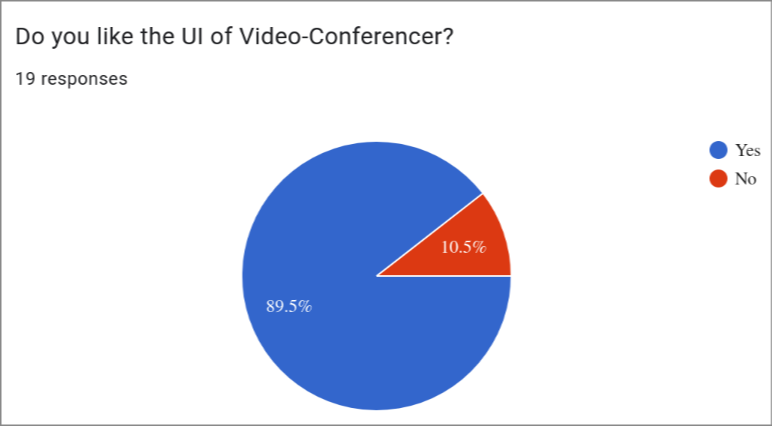
\includegraphics[scale=0.2]{Images/Survey.png}
\end{figure}

{\color{gray} \hrulefill} \\ \vspace{0.2cm}

Now that we have some of our core features implemented I thought that I should begin writing the documentation for
my system. Note that this ensures the completion of development sub-task \circled{1.3}. I chose to use Vitepress in
order to create a documentation site as it was simple to setup and had a nice modern looking UI out of the box. This
documentation will be sufficient to enable any future maintainers of the project to be able to understand the
code written. The documentation is written in markdown and looks like so:

\begin{minted}[linenos, bgcolor=lightestgray, breaklines, breakanywhere]{md}
# Tools

> [!NOTE]
> All of the tools that we use in Video-Conferencer have free tiers that we make use of.
> There may be better tools for these tasks that I don't know of or that require you
> to pay for them. Take my opinions with a grain of salt.

## Deployment
This was a project for my A-Level Computer Science coursework so naturally I didn't
want to pay money for a server to host my web application. Luckily there are a
number of services that allow us to host our applications on the cloud for free,
within certain limits.
...
\end{minted}

{\sffamily Tests: (17)}

\begin{itemize}
  \item System has proper documentation \faCheck
  \item Documentation is easy to read and access \faCheck
\end{itemize}

Here's what the site looks like: \\ \vspace{0.2cm}
{\sffamily Evidence}  \url{https://youtu.be/vLu_vxBv6rM} \\ \vspace{0.2cm}

With that we conclude the 4th iteration. \\ \vspace{0.2cm}

{\color{gray} \hrulefill} \\ \vspace{0.2cm}

{\sffamily Development sub-task \circled{1.3}} \faCheck \\ \vspace{0.2cm}

{\sffamily Development sub-task \circled{7}} \faCheck \\ \vspace{0.2cm}

{\sffamily Development sub-task \circled{8}} \faCheck \\ \vspace{0.2cm}

{\sffamily Development sub-task \circled{B}} \faCheck \\ \vspace{0.2cm}

Look at github commit \texttt{54eebbbc305fb6092a55973a82f040720c23872a} to see the state
of the project after our 4th iteration. \\ \vspace{0.2cm}

Alternatively click the following link to view the state of our project at this point in
development: \\
\href{https://github.com/zzzNathan/Video-Conferencer/tree/54eebbbc305fb6092a55973a82f040720c23872a}{\texttt{VideoConferencer-Iteration4}}

\section{Iteration 5}

In this iteration we are simply refining the system, finishing off documentation and creating the
helper document. I also implement one last featured, the events feature. Users will be able to add
events to their calendar then see all upcoming events in chronological order.
\\ \vspace{0.2cm}

I begin this iteration by refining the UI. I simplified some pages and touched up
designs to ensure consistency and clarity as well as create a prototype design for the events page.
The specific code changes can be viewed at the Github link provided at the end of this commit as usual.
Here is a video to summarise/demonstrate these UI changes. \\ \vspace{0.2cm}

{\sffamily Evidence:} \url{https://youtu.be/9vMbj_f_XJs} \\ \vspace{0.2cm}

I then worked on implementing the backend code in order to implement the events page. We have a table called
\texttt{Events} with the following structure. \\ \vspace{0.2cm}

\begin{center}
\begin{tikzpicture}

\pic{entity={logins}{\sffamily Logins}{
    \underline{Event\_Id} & \texttt{int} \\
    User\_Id & \texttt{string} \\
    Title & \texttt{string} \\
    Description & \texttt{string} \\
    Date & \texttt{date} \\
  }};

\end{tikzpicture}
\end{center}

\vspace{0.2cm}
Here's a rough sketch of what's going on in the backend:

\begin{itemize}
\item When the front end loads, we make a \texttt{POST} request to our backend, this returns a list of all of a user's events and we render these events on the front end. \\
\item When a user adds an event, we make a \texttt{PUT} request to our backend, this adds the new event data to our database. \\
\item When a user deletes an event we make \texttt{DELETE} request to our backend, this deletes that event from our database. \\
\end{itemize}

Here we present a code snippet of the most important functions,

\begin{minted}[linenos, bgcolor=lightestgray, breaklines, breakanywhere]{go}
...
// Get all of a user's events
func Get_Events(User_Id string) (string, error) {
    db, err := Connect()
    if err != nil {
        return "", err
    }
    defer db.Close() // Ensures connection closes once function returns

    // Query to get events ordered by date
    query := `
        SELECT event_id, user_id, title, description, date
        FROM events
        WHERE user_id = $1
        ORDER BY date DESC
    `

    // Execute query
    rows, err := db.Query(query, User_Id)
    if err != nil {
        return "", err
    }
    defer rows.Close()

    // Slice to hold all events
    var events []models.Event

    // Iterate through results
    for rows.Next() {
        var event models.Event
        err := rows.Scan(
            &event.Event_ID,
            &event.User_ID,
            &event.Title,
            &event.Description,
            &event.Date,
        )
        if err != nil {
            return "", err
        }
        events = append(events, event)
    }

    // Check for errors from iterating over rows
    if err = rows.Err(); err != nil {
        return "", err
    }

    // Convert to JSON
    Json_Data, err := json.Marshal(events)
    if err != nil {
        return "", err
    }

    return string(Json_Data), nil
}

// Get count of events for a user
func Get_Event_Count(User_Id string) (int, error) {
    db, err := Connect()
    if err != nil {
        return 0, err
    }
    defer db.Close()

    var count int
    query := `SELECT COUNT(*) FROM events WHERE user_id = $1`
    err = db.QueryRow(query, User_Id).Scan(&count)
    if err != nil {
        return 0, err
    }

    return count, nil
}

// Add a new event to the database
func Add_Event(Event models.Event) error {
    db, err := Connect()
    if err != nil {
        return err
    }
    defer db.Close()

    query := `
        INSERT INTO events (user_id, title, description, date)
        VALUES ($1, $2, $3, $4)
    `

    _, err = db.Exec(query, Event.User_ID, Event.Title, Event.Description, Event.Date)
    return err
}

// Delete an event from the database
func Delete_Event(Event_Id int, User_Id string) error {
    db, err := Connect()
    if err != nil {
        return err
    }
    defer db.Close()

    query := `
        DELETE FROM events
        WHERE event_id = $1 AND user_id = $2
    `

    _, err = db.Exec(query, Event_Id, User_Id)
    return err
}
\end{minted}

Given that our table was created with the following SQL,

\begin{minted}[linenos, bgcolor=lightestgray, breaklines, breakanywhere]{sql}
CREATE TABLE Events (
    event_id SERIAL PRIMARY KEY,
    user_id VARCHAR(255) NOT NULL,
    title VARCHAR(50) NOT NULL,
    description VARCHAR(200) NOT NULL,
    date DATE NOT NULL
);
\end{minted}

we do some \textbf{input validation} on the back end to ensure that the user only adds events that satisfy the restrictions for
the datatypes in this table. Here is an example from the \code{Handle\_Add\_Event()} function:

\begin{minted}[linenos, bgcolor=lightestgray, breaklines, breakanywhere]{go}
...
// Check event count
Event_Count, err := utils.Get_Event_Count(User_Id)
if err != nil {
    http.Error(w, "Failed to get event count: "+err.Error(), http.StatusInternalServerError)
    return
}

// Enforce event limit
if Event_Count >= MAX_EVENTS {
    http.Error(w, "Maximum event limit reached", http.StatusForbidden)
    return
}

// Parse JSON body into Event struct
var New_Event models.Event
if err := json.NewDecoder(r.Body).Decode(&New_Event); err != nil {
    http.Error(w, "Invalid request body: "+err.Error(), http.StatusBadRequest)
    return
}

// Override the User_Id from JSON with the one from header for security
New_Event.User_ID = User_Id

// Validate required fields
if New_Event.Title == "" || New_Event.Description == "" || New_Event.Date.IsZero() {
    http.Error(w, "Title, Description, and Date are required", http.StatusBadRequest)
    return
}

// Validate field lengths
if len(New_Event.Title) > MAX_TITLE_LENGTH {
    http.Error(w, fmt.Sprintf("Title must not exceed %d characters", MAX_TITLE_LENGTH), http.StatusBadRequest)
    return
}

if len(User_Id) > MAX_USER_ID_LENGTH {
    http.Error(w, fmt.Sprintf("User ID must not exceed %d characters", MAX_USER_ID_LENGTH), http.StatusBadRequest)
    return
}

if len(New_Event.Description) > MAX_DESCRIPTION_LENGTH {
    http.Error(w, fmt.Sprintf("Description must not exceed %d characters", MAX_DESCRIPTION_LENGTH), http.StatusBadRequest)
    return
}
\end{minted}

{\color{gray} \hrulefill} \\ \vspace{0.2cm}

{\sffamily Tests: (18)}

\begin{itemize}
  \item Users can properly add events to their account \faCheck
  \item Users events are saved to the database and are properly loaded on the front end \faCheck
  \item Users can properly delete events \faCheck
\end{itemize}

{\sffamily Evidence: } \url{https://youtu.be/yhekUnPFH08} \\ \vspace{0.2cm}

{\color{gray} \hrulefill} \\ \vspace{0.2cm}

\pagestyle{fancy} \rhead{\bfseries OCR A-Level Computer Science}
\chead{\mdseries \thepage}
\lhead{\bfseries Jonathan Kasongo \mdseries — May 2025/26}
\lfoot{\sffamily Candidate number: N/A}
\rfoot{\sffamily Centre number: N/A}

\chapter{Evaluation}
\label{chap:evaluation}

\section{Post-development testing}

Since we have a few features that I didn't consider when I created the original post-development test plan we begin
by creating a revised post-development test plan.

\subsubsection{Test 0}

{\sffamily Task:} Access documentation site. \\

{\color{gray} \hrulefill}

{\sffamily Test type: Normal.}

\begin{enumerate}
  \item Navigate to the site.
  \item Click on Docs.
\end{enumerate}

{\sffamily Expected outcome:} Documentation should load successfully. \\

{\color{gray} \hrulefill}

\subsubsection{Test 1}

{\sffamily Task:} Create an account.\\

{\color{gray} \hrulefill} \\

{\textit{Note that this test allows our user to see our login pages. This links to the usability feature
"Log in/Sign up page}}
\\ \vspace{0.2cm}

{\sffamily Test type: Normal.}

\begin{enumerate}
  \item Navigate to the sign up page.
  \item Enter an adequate username into the username field.
  \item Enter the password \texttt{if5\#@Jal} into the password field.
  \item Click on the sign up button.
\end{enumerate}

{\sffamily Expected outcome:} User account created successfully. \\

{\color{gray} \hrulefill}

{\sffamily Test type: Erroneous.}\\

\begin{enumerate}
\item Repeat the steps except use the password \texttt{AopS12v}.\\
\end{enumerate}

{\sffamily Expected outcome:} User account not created, display message saying password is too weak.\\

{\color{gray} \hrulefill}

{\sffamily Test type: Erroneous.} \\

\begin{enumerate}
\item Repeat the steps except use the password \texttt{123}.
\end{enumerate}

{\sffamily Expected outcome:} User account not created, display
message saying password is too weak.\\

{\color{gray} \hrulefill}

\vspace{0.2cm}

\subsubsection{Test 2}

{\sffamily Task:} Log in to your account.\\

{\color{gray} \hrulefill}

{\textit{Note that this test allows our user to see our login pages. This links to the usability feature
"Log in/Sign up page}} \\ \vspace{0.2cm}

{\sffamily Test type: Normal.}\\

\begin{enumerate}
  \item Navigate to the log in page.
  \item Enter your actual username into the username field.
  \item Enter your actual password into the password field.
  \item Click on the log in button.
\end{enumerate}

{\sffamily Expected outcome:} User logged in successfully. \\

{\color{gray} \hrulefill}

{\sffamily Test type: Erroneous.}\\

\begin{enumerate}
  \item Repeat the steps except using the wrong password.
\end{enumerate}

{\sffamily Expected outcome:} User not logged in,
message displaying "Wrong username or password!". \\

{\color{gray} \hrulefill}

{\sffamily Test type: Erroneous.}\\

\begin{enumerate}
  \item Repeat the steps except using the wrong username.
\end{enumerate}

{\sffamily Expected outcome:} User not logged in,
message displaying "Wrong username or password!". \\

{\color{gray} \hrulefill}

\vspace{0.2cm}

\subsubsection{Test 3}

{\sffamily Task:} Create an event.\\

{\color{gray} \hrulefill}

{\sffamily Test type: Normal.} \\

\begin{enumerate}
  \item Navigate to the events page \\
  \item Click on the create event button \\
  \item Create an event, then refresh the page to check whether the event saved. \\
\end{enumerate}

{\sffamily Expected outcome: } Event that was created should still be present after refreshing page. \\

{\color{gray} \hrulefill}

\subsubsection{Test 4}

{\sffamily Task:} Delete an event.\\

{\color{gray} \hrulefill}

{\sffamily Test type: Normal.} \\

\begin{enumerate}
  \item Navigate to the events page. \\
  \item Delete the event you just created. \\
  \item Refresh the page to verify the event was indeed deleted. \\
\end{enumerate}

{\sffamily Expected outcome: } Event was properly deleted, event doesn't show after refresh. \\

{\color{gray} \hrulefill}

\subsubsection{Test 5}

{\sffamily Task:} Start a video call.\\

{\color{gray} \hrulefill}

{\sffamily Test type: Normal.}\\

\begin{enumerate}
  \item Connect a webcamera and microphone to your device (if necessary).
  \item Navigate to the create call page.
  \item Click on the create call button.
\end{enumerate}

{\sffamily Expected outcome:} Unique call code generated successfully
and displayed to the user. User is able to view themselves in
the video call.\\

{\color{gray} \hrulefill}

\vspace{0.2cm}

\subsubsection{Test 6}

{\sffamily Task:} Join a video call.\\ \vspace{0.2cm}

\textit{This test requires 2 people. Both users should have a camera
and microphone connected to their device. Both users should have a
stable internet connection satisfying the requirements listed in section \ref{sec:hardware}}\\

{\color{gray} \hrulefill}

{\sffamily Test type: Normal.}\\

\begin{enumerate}
  \item Have person 1 complete the steps outlined in Test 5.
  \item Person 1 should share the unique call code with person 2.
  \item Person 2 should then navigate to the join call page and enter the code that they were given.
  \item Person 2 should click on the join call button.
\end{enumerate}

{\sffamily Expected outcome:} Both users successfully joined the video call
and can clearly see and hear each other.\\

{\color{gray} \hrulefill} \\

\subsubsection{Test 7}

{\sffamily Task:} Log out.\\

{\color{gray} \hrulefill}

{\sffamily Test type: Normal.}\\

\begin{enumerate}
  \item Navigate to your account profile.
  \item Click the log out button.
\end{enumerate}

{\sffamily Expected outcome:} User logged out. \\

{\color{gray} \hrulefill}

\vspace{0.2cm}

Once again once we complete the post-development test plan we will fill in the following feedback form

\begin{longtblr}[
  caption={Post-development feedback form.}
]{
  colspec={lXXX},
  row{1}={lightestgray}
}
  No & Question & Rating (1-10) & Additional comments \\
  1 & How easy was the task to complete? & ~ & ~ \\
  2 & How easy was it to navigate the site? & ~ & ~ \\
  3 & How would you rate the design of the site? & ~ & ~ \\
  4 & How would you rate the user experience of the site? & ~ & ~ \\
  5 & Any additional comments or suggestions & N/A & ~ \\
\end{longtblr}

{\sffamily Daniel:}\\ \vspace{0.2cm}

{\sffamily Evidence: \url{https://youtu.be/EZyeDKM6ZR8}} \\ \vspace{0.2cm}
{\sffamily Evidence: \url{https://youtu.be/QwnYLBzXy2Y}} \\ \vspace{0.2cm}
{\sffamily Evidence: \url{https://youtu.be/MS5u3zo47N8}} \\ \vspace{0.2cm}

Here is Daniel's feedback form: \\ \vspace{0.2cm}

\begin{longtblr}[
  caption={Post-development feedback form.}
]{
  colspec={lXlX},
  row{1}={lightestgray}
}
  No & Question & Rating (1-10) & Additional comments \\
  1 & How easy was the task to complete? & 8 & Very easy as the layout was very clear. However I would suggest tutorial pop ups under under some icons on the first time through when someone makes an account so they can see where everything is. \\
  2 & How easy was it to navigate the site? & 9 & Easy and friendly to the user \\
  3 & How would you rate the design of the site? & 9 & I personally really like the design, it's very professional and unique\\
  4 & How would you rate the user experience of the site? & 10 & The site does exactly what I expected and was quite seamless, I wouldn't expect any other user to face issues with it either \\
  5 & Any additional comments or suggestions & N/A & I wouldn't comment on anything else other than it was very user friendly \\
\end{longtblr}

From our post-developement testing we have \textbf{clearly} provided annotated evidence of post development testing
for function and robustness. Note that by getting Daniel's feedback form and by analysing his comments we gain
invaluable feedback for our usability features. \\

\section{Evaluating success criteria}

\newcommand{\evalone}{%
This web page is indeed designed in an intuitive and user
friendly manner, this is demonstrated through
it's clear structure and visual hierarchy.
Users are immediately drawn to the prominent
gradient-styled heading "Video conferencing" which effectively
communicates the platform's core purpose. They then have option
to click one of the call to action buttons to either sign up or
login immediately after viewing the heading, if they so choose.
Finally the user is provided with a variety of common actions
in the top navigation bar, so they can quickly and efficiently
access the information they require.
\textit{Reference:} {\sffamily Test (16)} \url{https://youtu.be/Ii8QkbziWo4}
}

\newcommand{\evaltwo}{%
For our log in
system we make use of Clerk, a thoroughly tested and widely used
API for handling the user log in feature. Since Clerk is an
industry standard API we assume that their infastructure is indeed
secure and completely compliant with GDPR regulations.
\textit{Reference:} Refer to
\url{https://clerk.com/docs/security/overview} for details. \\ \vspace{0.1cm}

On the other hand for our events system though no errors arised during
iterative testing, we have not created a rigorous security test for
this part of the back end code, hence why I have rated this criterion
at 50\% completion. \\ \vspace{0.1cm}

This issue could be addressed in the future by using security
tools like ZAP which scan your code and look for potential
security vulnerabilities. To ensure safety an external cyber-security
company could be hired to perform a detailed analysis on the system,
from which all of the security vulnerabilities could be dealt with.
}

\newcommand{\evalthree}{%
Though this success criteria point is completely subjective, I do believe that the designs ended up being professional
looking and aesthetically appealing. This claim is reinforced by the results of the survey we conducted. Indeed >89\%
of our surveyees said they like the design fullfilling the criteria stated in success criteria 3. This shows that my
opinion is the majority and many others also find the UI to be professional looking and aesthetically appealing.
\textit{Reference:} {\sffamily Test (16)} \url{https://youtu.be/Ii8QkbziWo4}
}

\newcommand{\evalfour}{%
I have met this success criteria completely by using the 100ms library to allow users to video conference with each
other. As was discussed in the development section I tried a few different methods before landing on 100ms, however
I believe that the solution I have found right now provides the simplest way of implementing video conferencing. The
backend simply makes an HTTP request to the 100ms servers to ask for host and guest codes to a room, once we have
recieved these codes we display a dialog box to the user informing them of the code that they can then share to others.
Other users then simply navigate to the join call page, enter the code and they will have joined the video conference.
This feature is indeed evidenced in iterative test 15 as seen below.
\textit{Reference:} {\sffamily Test (15)} \url{https://youtu.be/mX33jG6B1Ik} \url{https://youtu.be/D2J8Y2TnWjo}
}

\newcommand{\evalfive}{%
I have met this success criteria completely by using the Clerk API to handle our login system. By importing the
Clerk library and retrieving the API key using an environment variable we use Clerk's built-in login and registration
components to provide a modern and technically robust username and password system.
\textit{Reference:} {\sffamily Test (2)} \url{https://youtu.be/IjwQH1Z8aPw}
}

\newcommand{\evalsix}{%
I believe that we have partially met this success criterion. We have used Clerk to manage usernames and passwords
in our application. From our tests in the development section, Clerk seems to only verify whether or not the given
password is 8 or more characters. For some very common passwords Clerk prohibits the user from trying to make an
account and gives the output \texttt{This password has been found as part of a breach and can not be used, please
try another password instead.} However Clerk doesn't give any specific password requirements other than
\texttt{Your password must contain 8 or more characters.} \textit{Reference:} {\sffamily Test (2)}
\url{https://youtu.be/p-rWgn692KU} \\ \vspace{0.1cm}

To solve this issue we have a number of options. On the buisness plan Clerk actually allows us to enforce specific
password requirements (\url{https://clerk.com/blog/a-new-password-experience}), however this will cost us money and
we currently have no way to make any money back. We could also look into and reseach other username and password
management libraries in order to find alternatives, this will ensure that our username and password will still be
robust and secure, through usage of a thoroughly tested and reputable Javascript library. Finally if we have no other
solutions one could resort to implementing the username and password system themselves from scratch, however the
downside with this approach is that it may not be \textit{completely} secure, without comprehensive security testing,
this fact coupled with the truth that implementing such a system will take a good amount of time and resources
justifies it being the last resort option.
}

\newcommand{\evalseven}{%
I believe that we have not met this success criteria. For our video conferencing system we utilise the 100ms video
conferencing library, which means that any latency issues will not be resolvable on our end. In this manner the
latency of our video conferencing applciation is totally dependent on the perfomance of the 100ms servers at that
moment in time. Since we have no control over the performance of the 100ms servers we cannot ever be certain that
our video conferencing latency won't exceed 150ms, because the performance of the 100ms servers will be constantly
changing and varying due to a number of factors outside of our control. The fact that we cannot ever affirmatively
make the claim that our latency is below 150ms coupled with the fact that no real attempt was made to test the
latency of our application, constructs a detailed justification as to why I believe that success criteria 7 was not
met. \\ \vspace{0.1cm}

We now propose an idea to potentially resolve this issue. Since the amount of latency will be constantly varying it
makes sense to conduct tests on the performance of our system at regular intervals (perhaps each hour). To achieve
this we could write a script that accesses the website and starts a video conference with 2 bots and computes a
value for the average latency over a span of some $n$ seconds. Occasionally the 100ms servers will be down for
maintenance or due to an outage. In such a case we could notify our user on the home and landing pages of the status
of the 100ms servers.
}

\newcommand{\evaleight}{%
I believe that we have partially achieved success criteria 8. The explanation of the success criteria explicitly
states that we will measure the success of this criterion by conducting a test with 6 different participants, however
during our iterative and post-developement testing we only conducted tests with at most 2 different participants. The
system should be able to theoretically handle 6 participants easily, however due to various time and resource
constraints I was unable to conduct the test with 6 participants. We know that the system should theoretically be able
to handle $\geq$ 6 participants by analysing the following page and looking at the free tier specifically
\url{https://www.100ms.live/pricing}, moreover we have evidence to show that video conferencing with 2 people was
smooth and worked without issues. \textit{Reference: See Daniel's post-development testing.}\\ \vspace{0.1cm}

We now propose a potential resolution for this issue. We could ask some friends or family to try and help conduct this
test but aligning the schedules of 6 people for this 1 test could be tough. If this approach doesn't work we could
potentially create an online posting looking for testers, and give them some monetary incentive if they accept to be a
part of the testing.
}

\newcommand{\evalnine}{%
I believe that we have partially completed success criterion 9. In a similar manner to the previous criterion, the
system should theoretically be able to handle 500 user accounts. We know this by analysing this page specifically at
the free tier \textit{Reference:} \url{https://clerk.com/pricing}. Indeed according to this page we should be able to
handle 10000 monthly user accounts. However we have failed to conduct proper rigorous tests in order to acertain
whether or not system performance degrades after a certain number of users. \\ \vspace{0.1cm}

We now propose a potential solution to this issue. Getting 500 actual users to register an account could be
logistically difficult, so alternatively we could write a script that makes bots to register accounts on our website
programatically.
}

\begin{longtblr}[
  caption={Evaluation of the success criteria.}
]{
  colspec={l X[2] X[6] r},
  row{1}={lightestgray},
  row{2}={lightestgray},
  row{8}={lightestgray},
  rowhead=1
}
No & Criterion & Evaluation & \% \\
{\sffamily Qualitative} & & & \\
1 & System should be intuitive and easy to grasp & \evalone & 100\% \\
2 & The user's data should be properly secured & \evaltwo & 50\% \\
3 & The webpage design should be aesthetically pleasing & \evalthree & 100\% \\
4 & Users should be able to create and join video conferences & \evalfour & 100\% \\
5 & Users should be able to create, login and logout of their own accounts & \evalfive & 100\% \\
{\sffamily Quantitative} & & & \\
6 & User passwords should be of an adequate strength & \evalsix & 50\% \\
7 & The video call latency should not exceed 150ms & \evalseven & 0\% \\
8 & The system should be able to handle video conferences with more than 2 participants & \evaleight & 50\% \\
9 & The system should be able to store at least 500 user accounts & \evalnine & 50\% \\
\end{longtblr}

\section{Evaluation of the usability features}

\newcommand{\usaone}{%
I believe that we have completed this feature completely, as we recall designing and implementing
the home page in the development section. The final design uses React and JSX to render the front end.
\textit{Reference:} \sffamily{Test (2)}
}

\newcommand{\usatwo}{%
I believe that we have completed this feature completely, as we have designed and implemented
a log in page as well as a sign up page in our development section. The final design makes use of the Clerk SDK to
hanle the registration and login logic, and the front end is implemented with React. \textit{Reference:}
\sffamily{Test (3)}
}

\newcommand{\usathree}{%
I believe that we have not completed this feature. Due to time constraints we unfortunately
could not get to creating a helper document. \\ \vspace{0.1cm} We note that this issue is rather easy to fix, since
we could simply ask the IT staff at my client's workplace to create the document. This will fully resolve the issue.
}

\newcommand{\usafour}{%
I believe that we have not completed this feature. Due to time constraints we were not able to implement
this feature. \\ \vspace{0.1cm} Implementing macros inside the video conferencing system is not a trivial task at all,
since we are making use of the 100ms library. From my understanding the 100ms library
}

\newcommand{\usafive}{%
I believe that we have not completed this feature. Due to time constraints we were not able to
implement this feature.
}

% Give evidence via video, commentate them with usability features
\begin{longtblr}[
  caption={Evaluation of the usability features.}
]{
  colspec={l X[2] X[6] r},
  row{1}={lightestgray},
  rowhead=1
}
No & Feature & Evaluation & \% \\
1 & Home page & \usaone & 100\% \\

2 & Log in/Sign up page & \usatwo & 100\% \\

3 & Help PDF document & \usathree & 0\% \\

4 & Macros & \usafour & 0\% \\

5 & Video tutorial & \usafive & 0\% \\
\end{longtblr}

\section{Limitations}

We begin by discussing the limitations that we considered in our analysis section \ref{sec:limitations}.

\subsection{Initial limitations}

\subsubsection{Internet}

Indeed as we explored in our analysis an internet connection is necessary for the user to be able to access our system.
As previously discussed we notice that the requirement of having a stable internet connection could potentially
restrict some users with poor economic situations from using our system. Indeed this opposes the initial motivation
for this project: to create an \textit{accessible} video conferencing application. \\ \vspace{0.2cm}

Though the requirement to have a stable internet connection has it's negatives, we argue that it is necessary since
there are no realistic solutions to this limitation. Indeed in order to conduct video conferencing users will have to
send video and/or audio data to the other users in the conference one way or another, there is no arguing this fact.
In this time period \footnote{At the time of writing the year is currently 2025} we have 2 main methods of data
communication. The first is to send signals over a WAN like the internet. The second is to physically connect devices
together in a LAN. If the first option is off the table we can only employ the second option. We note that the second
option requires a much more tedious setup as well as requires each user to be in relatively close proximity to all
the other users in the video conference. These inconveniences far outweigh the inconveniece of having to purchase and
install a stable internet connection.

\subsubsection{Passwords}

We previously discussed the issue of users forgetting their own passwords and getting logged out of their accounts.
Though we understand that we can never fix this issue totally, we argue that we have derived a partial solution.
\\ \vspace{0.2cm}

In using the Clerk library in order to handle our user management systems, we note that they allow our users to be
able to login to our system using their google accounts. Using their google accounts the user doesn't need to remember
their password as they may simply click on the "Continue with Google" button after which they will be able to easily
sign in using their Gmail. \\ \vspace{0.2cm}

\subsubsection{Signalling servers}

When we initially wrote the limitations section, I assumed that I would be working with WebRTC library in order to
facilitate the implementation of video conferencing in our application. However in the final solution we note that we
instead make use of the 100ms video conferencing library. Not only does this library provide a much simpler method
to implement video conferencing it also renders the system much more maintainable as our maintainers will have a lot
less work to complete if the system isn't too complex. \\ \vspace{0.2cm}

With that it is easy to see that this limitation no longer applies to us.

\subsubsection{Social engineering}

We construct a philosophical arguement to justify the claim that we can never truly guarentee that this issue is
resolved. Due to human nature we understand that in the 21st century we can never completely eliminate the effect of
evil. Robert Greene argues in his book \textit{The 48 Laws of Power} that humans act only for their own benefit
\cite{power}, so if a situation arises in which someone obtains sufficient motivation to commit an act of evil,
in this case the use of social engineering to obtain somebody else's password, then in their eyes such an act doesn't
become morally injust anymore. Thomas Hobbes reinforces this school of thought in his book \textit{Leviathan} \cite{lev}.
He argues that man is naturally self-interested, implying that what we might think of as evil could be an inevitable
result of man's struggle for survival. Moreover we note that every human sees the world differently and consequently
has their own morals and views as a result of their experiences. As man wanders through life and encounters new
experiences his thoughts and morals will constantly morph and shift. In this manner our struggle against evil is not
a discrete one-time battle but is rather a continous everlasting commitment to fighting for one's own views of morally
just and injust.
\\ \vspace{0.2cm}

In order stop humans from commiting such acts we would have to monitor and restrict the actions of each and every one
of the $\approx$ 8 million people on earth. Such drastic measures would not only be \textbf{extremely} resource
intensive for my client and his small team but would also be morally dubious to the point where it could perhaps
illicit global-scale actions in response. This reasoning alone is enough to justify the fact that this limitation can
never \textbf{truly} be fixed. \\ \vspace{0.2cm}

We now discuss some new limitations that were not considered in the analysis section.

\subsection{New limitiations}

\subsubsection{Helper document}

Unfortunately we were unable to create the helper document that we spoke of in section \ref{sec:usability} due to
time constraints in our development sections. Since we lack a \textit{user guide} it may be difficult for new users
to understand where everything is and what features exist in the system, this was highlighted in Daniel's critique:
\textit{"I would suggest tutorial pop ups under
under some icons on the first time through
when someone makes an account so they
can see where everything is."} However we hope that the simple design of our system compensates for the
lack of a helper document as most users should be able to understand how to use and navigate the software, this
conclusion is justified by the feedback we recieved from Daniel during our post-development testing, where he
explicity mentioned how easy the software was to use: \textit{"Very easy as the layout was very clear."}. \\
\vspace{0.2cm}

Thankfully this limitation can easily be remedied by asking one of the IT staff at our client's place of work to create
a helper document, and then implement a button on the navbar that allows the users to click and have the helper
document open up in another tab.

\subsubsection{Landing page}

The final landing page design ended up being simple and professional looking, however there are still improvements
to be made. The landing page should demonstrate some of the core features of our application whilst remaining
professional looking, modern and eye-catching.

\section{Maintenance}

\appendix

\chapter{Code listings}

\section{Front end}

\underline{src/components/Events.jsx}

\inputminted[linenos, bgcolor=lightestgray, breaklines, breakanywhere]{jsx}{../Video-Conferencer/src/components/Events.jsx}

\underline{src/components/Home.jsx}

\inputminted[linenos, bgcolor=lightestgray, breaklines, breakanywhere]{jsx}{../Video-Conferencer/src/components/Home.jsx}

\underline{src/components/Join\_Call.jsx}

\inputminted[linenos, bgcolor=lightestgray, breaklines, breakanywhere]{jsx}{../Video-Conferencer/src/components/Join_Call.jsx}

\underline{src/components/Landing.jsx}

\inputminted[linenos, bgcolor=lightestgray, breaklines, breakanywhere]{jsx}{../Video-Conferencer/src/components/Landing.jsx}

\underline{src/components/Loading.jsx}

\inputminted[linenos, bgcolor=lightestgray, breaklines, breakanywhere]{jsx}{../Video-Conferencer/src/components/Loading.jsx}

\underline{src/components/Login.jsx}

\inputminted[linenos, bgcolor=lightestgray, breaklines, breakanywhere]{jsx}{../Video-Conferencer/src/components/Login.jsx}

\underline{src/components/Navbar.jsx}

\inputminted[linenos, bgcolor=lightestgray, breaklines, breakanywhere]{jsx}{../Video-Conferencer/src/components/Navbar.jsx}

\underline{src/components/Registration.jsx}

\inputminted[linenos, bgcolor=lightestgray, breaklines, breakanywhere]{jsx}{../Video-Conferencer/src/components/Registration.jsx}

\underline{src/components/Video\_Call.jsx}

\inputminted[linenos, bgcolor=lightestgray, breaklines, breakanywhere]{jsx}{../Video-Conferencer/src/components/Video_Call.jsx}

\section{Back end}

\underline{Call-Manager/api/provider.go}

\inputminted[linenos, bgcolor=lightestgray, breaklines, breakanywhere]{jsx}{../Call-Manager/api/provider.go}

\underline{Call-Manager/libs/utils.go}

\inputminted[linenos, bgcolor=lightestgray, breaklines, breakanywhere]{jsx}{../Call-Manager/libs/utils.go}

\underline{Event-Manager/api/events.go}

\inputminted[linenos, bgcolor=lightestgray, breaklines, breakanywhere]{jsx}{../Event-Manager/api/events.go}

\underline{Event-Manager/lib/handlers/handler.go}

\inputminted[linenos, bgcolor=lightestgray, breaklines, breakanywhere]{jsx}{../Event-Manager/lib/handlers/handler.go}

\underline{Event-Manager/lib/models/event.go}

\inputminted[linenos, bgcolor=lightestgray, breaklines, breakanywhere]{jsx}{../Event-Manager/lib/models/event.go}

\underline{Event-Manager/lib/utils/database.go}

\inputminted[linenos, bgcolor=lightestgray, breaklines, breakanywhere]{jsx}{../Event-Manager/lib/utils/database.go}


\printbibliography

\end{document}
